\documentclass [11pt,twoside]{article}
\usepackage[shortlabels]{enumitem}
\usepackage{array}
\usepackage{hyperref}
\usepackage{multirow}
\usepackage{tabularray}
\usepackage[dvipsnames]{xcolor}
\usepackage{listings}
\renewcommand{\arraystretch}{1.3}
\documentclass [11pt,twoside]{article}
\usepackage[utf8]{inputenc}
\usepackage[T1]{fontenc}

%Page margins, header and footer positions
\usepackage{geometry}
 \geometry{
 a4paper,
 total={210mm,297mm},
 left=25mm,
 right=25mm,
 top=30mm,
 bottom=25mm,
 headsep=7mm}

\interfootnotelinepenalty=10000

%To display filling dots in the TOC for all entries
\usepackage[titles]{tocloft}
\renewcommand{\cftsecleader}{\cftdotfill{\cftdotsep}}

%Define new header and footer style
\usepackage{fancyhdr}

\pagestyle{fancy}
\fancyhf{}
\lhead{\color{Gray}{\small{Travlendar+ project by YOUR NAMES}}}
\lfoot{\textcolor{Gray}{\small{Copyright © 2017, YOUR NAMES – All rights reserved}}}
\rfoot{\textcolor{Gray}{\thepage}}
\renewcommand{\headrulewidth}{0pt}

%PACKAGES
\usepackage{wasysym}
\usepackage{pifont}

\newcommand{\supported}{\ding{52}\xspace}
\newcommand{\unsupported}{\ding{55}\xspace}
\newcommand{\partsupported}{\textcolor{black!40}{\ding{52}}\xspace}
\newcommand{\lowsupported}{\textcolor{black!20}{\ding{52}}\xspace}
\newcommand{\unknowsupported}{\textbf{?}\xspace}

%Font: Times
\usepackage{times}
%Change monospaced font
\renewcommand{\ttdefault}{lmtt}

%tables
\usepackage{tabu}
\usepackage{tabularx}
\usepackage{ltablex}
\usepackage{longtable}
\usepackage{float} % To allow the use of H modifier in long tables

%landscape mode
\usepackage{pdflscape}
\usepackage{rotating}
\usepackage{caption}

%make landscape mode be sensitive to even and odd pages
%start
\def\myrotate{\ifodd\c@page\else-\fi 90}
\makeatletter
\global\let\orig@begin@landscape=\landscape%
\global\let\orig@end@landscape=\endlandscape%
\gdef\@true{1}
\gdef\@false{0}
\gdef\landscape{%
    \global\let\within@landscape=\@true%
    \orig@begin@landscape%
}%
\gdef\endlandscape{%
    \orig@end@landscape%
    \global\let\within@landscape=\@false%
}%
\@ifpackageloaded{pdflscape}{%
    \gdef\pdf@landscape@rotate{\PLS@Rotate}%
}{
    \gdef\pdf@landscape@rotate#1{}%
}
\let\latex@outputpage\@outputpage
\def\@outputpage{
    \ifx\within@landscape\@true%
        \if@twoside%
            \ifodd\c@page%
                \gdef\LS@rot{\setbox\@outputbox\vbox{%
                    \pdf@landscape@rotate{-90}%
                    \hbox{\rotatebox{90}{\hbox{\rotatebox{180}{\box\@outputbox}}}}}%
                }%
            \else%
                \gdef\LS@rot{\setbox\@outputbox\vbox{%
                    \pdf@landscape@rotate{+90}%
                    \hbox{\rotatebox{90}{\hbox{\rotatebox{0}{\box\@outputbox}}}}}%
                }%
            \fi%
        \else%
            \gdef\LS@rot{\setbox\@outputbox\vbox{%
                \pdf@landscape@rotate{+90}%
                \hbox{\rotatebox{90}{\hbox{\rotatebox{0}{\box\@outputbox}}}}}%
            }%
        \fi%
    \fi%
    \latex@outputpage%
}
\makeatother
%end

%graphics
\usepackage{graphicx}
\usepackage[dvipsnames, table]{xcolor}
%If you upload images from PC, you need to insert code for the path here (different for Windows and Unix OS)

%References
%\usepackage{xpatch}
%\usepackage[backend=biber, style=numeric, citestyle=numeric, sorting=none]{biblatex}
%\addbibresource{main.bib}

%Other
\usepackage{ifthen}
\usepackage{xspace}
\usepackage{enumitem}
\usepackage{amssymb}
\usepackage[pdftex, colorlinks]{hyperref}
\newcommand{\comment}[1]{{\color{Red}$\blacktriangleright$ Comment: #1 $\blacktriangleleft$}}


% Some utilities\ldots
\usepackage{soul}
\usepackage{tikz}

\usetikzlibrary{calc}
\usetikzlibrary{decorations.pathmorphing}


\makeatletter

\newcommand{\defhighlighter}[3][]{%
  \tikzset{every highlighter/.style={color=#2, fill opacity=#3, #1}}%
}

\defhighlighter{yellow}{.5}

\newcommand{\highlight@DoHighlight}{
  \fill [ decoration = {random steps, amplitude=1pt, segment length=15pt}
        , outer sep = -15pt, inner sep = 0pt, decorate
       , every highlighter, this highlighter ]
        ($(begin highlight)+(0,8pt)$) rectangle ($(end highlight)+(0,-3pt)$) ;
}

\newcommand{\highlight@BeginHighlight}{
  \coordinate (begin highlight) at (0,0) ;
}

\newcommand{\highlight@EndHighlight}{
  \coordinate (end highlight) at (0,0) ;
}

\newdimen\highlight@previous
\newdimen\highlight@current

\DeclareRobustCommand*\highlight[1][]{%
  \tikzset{this highlighter/.style={#1}}%
  \SOUL@setup
  %
  \def\SOUL@preamble{%
    \begin{tikzpicture}[overlay, remember picture]
      \highlight@BeginHighlight
      \highlight@EndHighlight
    \end{tikzpicture}%
  }%
  %
  \def\SOUL@postamble{%
    \begin{tikzpicture}[overlay, remember picture]
      \highlight@EndHighlight
      \highlight@DoHighlight
    \end{tikzpicture}%
  }%
  %
  \def\SOUL@everyhyphen{%
    \discretionary{%
      \SOUL@setkern\SOUL@hyphkern
      \SOUL@sethyphenchar
      \tikz[overlay, remember picture] \highlight@EndHighlight ;%
    }{%
    }{%
      \SOUL@setkern\SOUL@charkern
    }%
  }%
  %
  \def\SOUL@everyexhyphen##1{%
    \SOUL@setkern\SOUL@hyphkern
    \hbox{##1}%
    \discretionary{%
      \tikz[overlay, remember picture] \highlight@EndHighlight ;%
    }{%
    }{%
      \SOUL@setkern\SOUL@charkern
    }%
  }%
  %
  \def\SOUL@everysyllable{%
    \begin{tikzpicture}[overlay, remember picture]
      \path let \p0 = (begin highlight), \p1 = (0,0) in \pgfextra
        \global\highlight@previous=\y0
        \global\highlight@current =\y1
      \endpgfextra (0,0) ;
      \ifdim\highlight@current < \highlight@previous
        \highlight@DoHighlight
        \highlight@BeginHighlight
      \fi
    \end{tikzpicture}%
    \the\SOUL@syllable
    \tikz[overlay, remember picture] \highlight@EndHighlight ;%
  }%
  \SOUL@
}

\makeatother

% Common abbrev. are set as commands to ensure proper spacing after the dot
\RequirePackage{xspace}
\newcommand{\ie}{i.e.\@\xspace}
\newcommand{\aka}{a.k.a.\@\xspace}
\newcommand{\Ie}{I.e.\@\xspace}
\newcommand{\cf}{cf.\@\xspace}
\newcommand{\Cf}{Cf.\@\xspace}
\newcommand{\eg}{e.g.\@\xspace}
\newcommand{\Eg}{E.g.\@\xspace}
\newcommand{\etal}{et al.\@\xspace}
\newcommand{\etc}{etc.\@\xspace}
\newcommand{\wrt}{w.r.t.\@\xspace}
\newcommand{\Wrt}{W.r.t.\@\xspace}



\date{}


\begin{document}

%TITLE PAGE

\begin{titlepage}


%LOGO

\begin{table}[t!]
\centering
\begin{tabu} to \textwidth { X[c] }

\includegraphics[scale=0.5]{Images/PolimiLogo} \\
\textbf{\small{Dipartimento di Elettronica, Informazione e Bioingegneria}} \\ 
\textbf{\small{Software Engineering 2}} \\
\end{tabu}
\end{table} ~
\\ [4cm]

%TITLE 

\begin{center}
    %Replace the text string with your title
{\textbf{\Huge{CodeKataBattle}}} \\ 
\vspace{2mm}
{\textbf{\small{Design Document}}} \\ 
{\textbf{\footnotesize{Version 1}}} \\ [4cm]
\textbf{\small{Mehmet Emre Akbulut}} \\
\vspace{1mm}
\textbf{\small{Yavuz Samet Topcuoglu}} \\ [1cm]
\textbf{\footnotesize{07 January 2024}}
\end{center}





\end{titlepage}

%Define deliverable specific info
%Replace cell contents where needed
\begin{table}[h!]
\begin{tabu} to \textwidth { X[0.3,r,p] X[0.7,l,p] }
\hline

\textbf{Deliverable:} & DD\\
\textbf{Title:} & CodeKataBattle - Design Document \\
\textbf{Authors:} & Mehmet Emre Akbulut, Yavuz Samet Topcuoglu \\
\textbf{Version:} & 1.0 \\ 
\textbf{Date:} & 07 January 2023 \\
\textbf{Download page:} & \href{https://github.com/mehmetemreakbulut/AkbulutTopcuoglu}{GitHub Repository} \\
\textbf{Copyright:} & Copyright © 2023, Akbulut \& Topcuoglu – All rights reserved \\
\hline
\end{tabu}
\end{table}




\setcounter{page}{2}


%------------------------------------------------------------------------------------------------------------------------------------------------
\newpage
\addcontentsline{toc}{section}{Table of Contents}
\tableofcontents
\newpage
\addcontentsline{toc}{section}{List of Figures}
\listoffigures
\addcontentsline{toc}{section}{List of Tables}
\listoftables

%------------------------------------------------------------------------------------------------------------------------------------------------
\clearpage
{\color{Blue}{\section{Introduction}}}
\label{sect:introduction}

\subsection{Purpose}
In today's digital age, education has evolved significantly, with online learning becoming more and more important, especially in subjects like computer science. However, only theoretical learning often can be insufficient in practical fields like coding. This is where the CodeKataBattle (CKB) project steps in, addressing the need for a hands-on, collaborative, and engaging approach to learning programming and software development.


Although theoretical knowledge is essential in computer science, it is the practical application and coding practice that strengthen students' understanding and skills. Hence, CKB is designed to support students with a platform where they can actively practice coding, experiment, learn from their mistakes, and improve their skills. Moreover, it encourages students to work together in teams, promoting teamwork and communication, essential qualities in the software development field. For educators, CKB offers a valuable teaching tool, enabling them to create coding challenges in accordance with their curricula, making learning more engaging, and helping assess students' progress.


In summary, the CodeKataBattle project serves as a bridge between theoretical learning and practical application in computer science education. It offers students a platform to practice coding, collaborate, and improve their skills, and provides educators with effective teaching tools and assessment methods. The aim of CKB is to make computer science education more engaging, practical, and rewarding for both students and educators.

\subsubsection{Goals}

\begin{enumerate}

 \item Educators are able to prepare and manage programming exercises.
 \item Educators are able to work collaboratively to create coding exercises.
 \item Students are able to participate in programming exercises individually or with a team.
 \item Students are able to get evaluations for their coding solutions, enhancing their learning experience.
 \item Educators are able to compare students' performance based on certain programming exercises.

 
 





% \item  Students can view their rankings on their profiles.
\end{enumerate}

\subsection{Scope}

\subsubsection{Product Identification}

\begin{itemize}

    \item The \textbf{target audience} of the platform is mainly \textbf{students and educators} in computer science and related fields. 
    
    \item CKB is an \textbf{interactive web-based coding platform} specifically designed to improve the coding skills of students by participating in battles designed by educators. It is mainly an \textbf{educational tool} where practice can be applied.

    \item CKB is also a \textbf{competitive learning environment}. By organizing the coding exercises in battle format, the students are expected to be more motivated to perform their best in challenges.

    \item The platform \textbf{promotes teamwork and collaboration} by allowing students to form groups to tackle battles together. This reflects real-world software development scenarios where collaborative team dynamics are key.

    \item The platform has an \textbf{educator-centric control}. The educators play a crucial role in the platform because they are the ones creating, managing, and scoring the battles and tournaments.

    \item CKB enables students to \textbf{use professional tools and practices} such as version control, and fork-pull-push mechanisms so that they can enhance their real-world software development skills with the help of Github.

    \item The platform makes use of \textbf{automated testing} to assess student submissions, ensuring objective evaluation of functional correctness and code quality. Additionally, it allows educators to perform manual evaluations for aspects that require subjective judgment.

    \item CKB is designed to provide \textbf{instant feedback} on submissions and \textbf{real-time updates} of team scores and rankings.

    \item The platform offers \textbf{flexibility} to educators in terms of the choice of programming languages, difficulty levels of challenges, and the scope of coding tasks, making it adaptable to various learning curves and educational needs.

    
\end{itemize}

\subsubsection{Domain Analysis}
The CKB platform operates within the domain of educational technology, specifically tailored for coding and software development education. From this perspective, we have the following users:

Educators:
Educators use CKB to \textbf{create and manage coding exercises}, known as code katas, in a battle format. They have the capability to set parameters for these exercises, including difficulty levels, deadlines, and specific technical requirements. Educators can \textbf{evaluate student submissions} both automatically (using the platform's tools) and manually, \textbf{providing feedback and scores}.

Students:
Students exploit the platform to enhance their coding skills by \textbf{participating} in these code battles. They work individually or in teams to solve the challenges set by educators, fostering both individual and collaborative learning experiences. Students use the platform \textbf{to submit their code, receive real-time feedback, and track their progress in coding proficiency}.

In summary, the domain of the CKB platform is focused on interactive, competitive coding education, enabling students to have an engaging learning experience while offering educators powerful tools for managing and evaluating coding exercises.

\subsubsection{World Phenomena}

\begin{enumerate}
    \item Educators prepare and manage programming exercises to assess students.
    \item Educators prepare test cases and build scripts related to their programming exercises.
    \item Educators can work collaboratively to provide exercises to the students.
    \item Students participate in programming exercises to improve their programming skills.
    \item Students will to compare themselves on coding challenges.
    \item Students can work collaboratively to provide solutions to exercises.
    \item Students fork the code repositories.
    \item Students set up an automated workflow.
    \item Students write code on their devices.
    \item Educators evaluate students based on their solutions to the programming exercises.
    \item Educators decide on some quality aspects to assess students.
    \item Educators compare students based on their success in certain coding exercises. 
    \item Students get evaluations for their solutions to the coding exercises. 
\end{enumerate}

\subsubsection{Shared Phenomena}


\quad \space \space \textbf{World Controlled}
\begin{enumerate}
    \item Educators create coding challenges, including descriptions and test cases, for the platform.
    \item Educators create tournaments and give permission to their colleagues to create battles for that tournament.
    \item Educators set specific rules and criteria such as deadlines, number of team members, and additional configurations for scoring for code kata battles.
    \item Educators decide on the inclusion of manual scoring components for battles and score manually.
    \item Students invite peers to form teams within the platform or join individually in the battles.
    \item Students submit their code solutions by pushing the code via GitHub.
    
\end{enumerate}

\textbf{Machine Controlled}
\begin{enumerate}[resume]
    \item The CKB platform sends notifications to students about new battles and tournaments, invitations, final battle ranks, and final tournament ranks.
    \item The platform generates and manages GitHub repositories for each battle and sends links to students that are participating.
    \item The CKB platform automatically evaluates code submissions against test cases, timeliness, and quality aspects.
    \item The platform updates battle scores and battle rankings in real-time.
    \item The platform displays leaderboards (i.e. the rank of the sum of all battle scores received in that tournament).
\end{enumerate}

\subsection{Definitions, Acronyms, Abbreviations}

\subsubsection{Definitions}
\begin{itemize}
    \item \textbf{Student}: An individual enrolled in an educational program or course who uses the platform to participate in coding exercises and improve software development skills.
    \item \textbf{Educator}: A person, such as a teacher or an instructor, responsible for creating coding challenges and managing learning activities on the platform.
    \item \textbf{Automated Testing}: A process where the CKB platform automatically executes predefined tests on student code submissions to assess their functionality and correctness without manual intervention.
    \item \textbf{Manual Scoring}: The process where educators evaluate student code submissions subjectively, complementing the automated testing system.
    \item \textbf{Battle}: A competitive coding challenge on the platform where students or teams of students solve specific programming problems within set parameters and time frames.
    \item \textbf{Tournament}: A series of code kata battles organized and managed by educators on the CKB platform, that ranks students or teams based on cumulative scores from individual battles.
    \item \textbf{Ranking}: A system within the CKB platform that orders participating students or teams based on their performance in individual code kata battles, determined by scores from automated and manual evaluations.
    \item \textbf{Leaderboard}: A feature on CKB that displays the standings of students or teams based on their performance overall in a tournament.
    \item \textbf{Institution Information}: Institution Information is multiple choice of institutions for the educators, a single institution for the students.
    \item \textbf{Unregistered User}: Users that haven't registered to the platform yet.
    \item \textbf{Registered User}: User that have registered to the platform.
    \item \textbf{Authenticated User}: User that have logged in to the platform.
    \item \textbf{Availability}: Availability is the status of tournament in terms of Closed, Open, or Upcoming.
    \item \textbf{Own Tournaments}: Own Tournaments means the tournaments they created from  Educator perspective, on the other hand, it means the tournaments they registered from  Student perspective.
    \item \textbf{Own Battles}: Own Battles means the battles they created from  Educator perspective, on the other hand, it means the battles they registered from  Student perspective.
    \item \textbf{Scoring Criteria}: Scoring Criteria includes Test Cases, Timeliness and Quality.
    

\end{itemize}

\subsubsection{Acronyms}
\begin{itemize}
    \item \textbf{CKB}: CodeKataBattle
\end{itemize}

\subsubsection{Abbreviations}
\begin{itemize}
    \item $G_{x}$: x-th Goal
    \item $WP_{x}$: x-th World Phenomena
    \item $SP_{x}$: x-th Shared Phenomena
    \item $D_{x}$: x-th Domain Assumption
    \item $SC_{x}$: x-th Statechart
    \item $AD_{x}$: x-th Activity Diagram
    \item $UC_{x}$: x-th Use Case
    \item $SD_{x}$: x-th Sequence Diagram
    \item $R_{x}$: x-th Functional Requirement
    \item $NFR_{x}$: x-th Non-Functional Requirement
\end{itemize}

%------------------------------------------------------------------------------------------------------------------------------------------------
\clearpage
{\color{Blue}{\section{Architectural Design}}}
\label{sect:architecture}
\subsection{Overview}

The high-level architectural diagram provided below offers a conceptual overview of the CodeKataBattle (CKB) platform's infrastructure. It delineates the system's division into three primary layers: Presentation, Application, and Data. 

The Presentation Layer captures the user interaction with the system via a standard web browser, illustrating the entry point for both educators and students. 

The Application Layer is the system's backbone, housing the business logic and core functionalities, including load balancing, application servers, and interfaces for external services such as the GitHub API, Static Analysis Tool API, Email Service, and Notification Service. A dedicated firewall protects this layer, ensuring secure data transactions. 

The Data Layer is structured to manage persistent data and comprises the Database Management System (DBMS), which supports sharded databases for scalability, and a File Storage system that accommodates various data types, including educator uploads and code submissions. 

Each component is strategically placed to optimize performance and maintainability, reinforcing the platform’s robustness and reliability.

\begin{figure}[H]
    \centering
    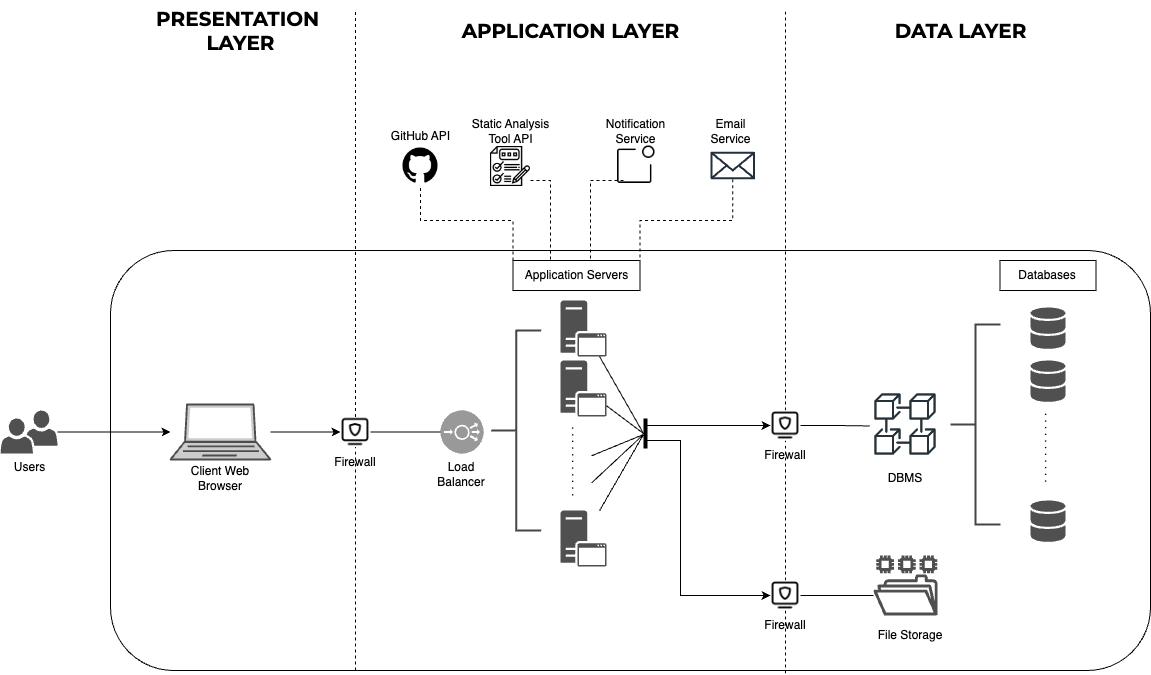
\includegraphics[width=\linewidth]{Images/hl-architecture.drawio.png}
    \caption{High-Level Architecture of the System}
\end{figure}


\subsection{Component View}




\subsection{Deployment View}






\subsection{Runtime View}




\subsection{Component Interfaces}



\subsection{Selected Architectural Styles and Patterns}




\subsection{Other Design Decisions}




%------------------------------------------------------------------------------------------------------------------------------------------------
\clearpage
{\color{Blue}{\section{User Interface Design}}}
\label{sect:ui}
In this section, we present user interfaces for Students and Educators. We created a detailed user interface design to inform the reader from a broader perspective.  It provides a clear understanding of how the end-user will interact with the software. This visual representation can demonstrate the flow and layout of the application, making it easier for stakeholders to grasp the user experience. In the UI design we aim to serve as a common language for all stakeholders, including developers, designers, project managers, and clients. It helps in bridging the gap between non-technical and technical team members with help of graphical demonstration. We tried to create every screen possible in order to inform to developers and stakeholders as much as possible. Developer can simplify and advance this user interface designs if they needed.
\\
Naturally runtime views contain much information however user design shows the application from students and educators. However, every mockup is somehow related to a runtime view. Related runtime views are shown.

\begin{center}
    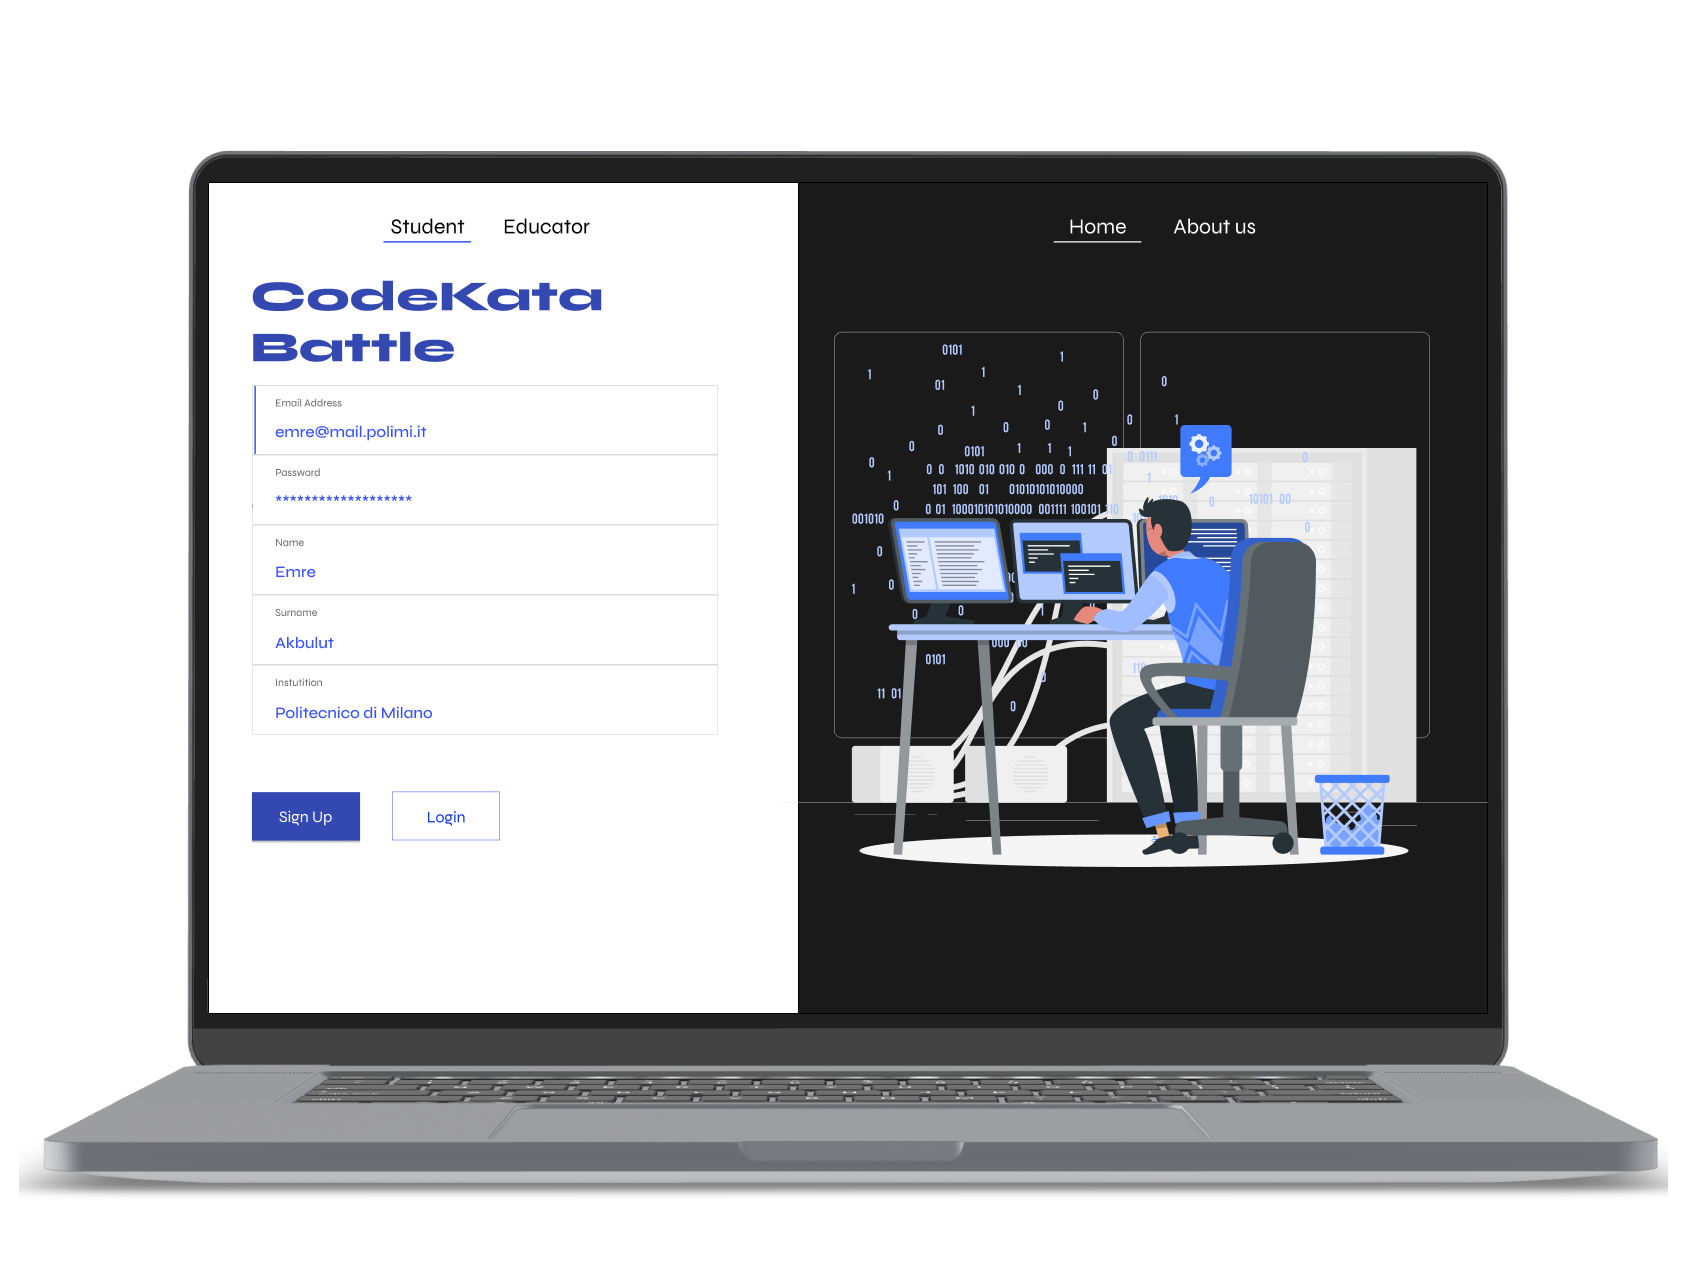
\includegraphics[scale=0.13]{Images/ui-ux/student_signup.png}
    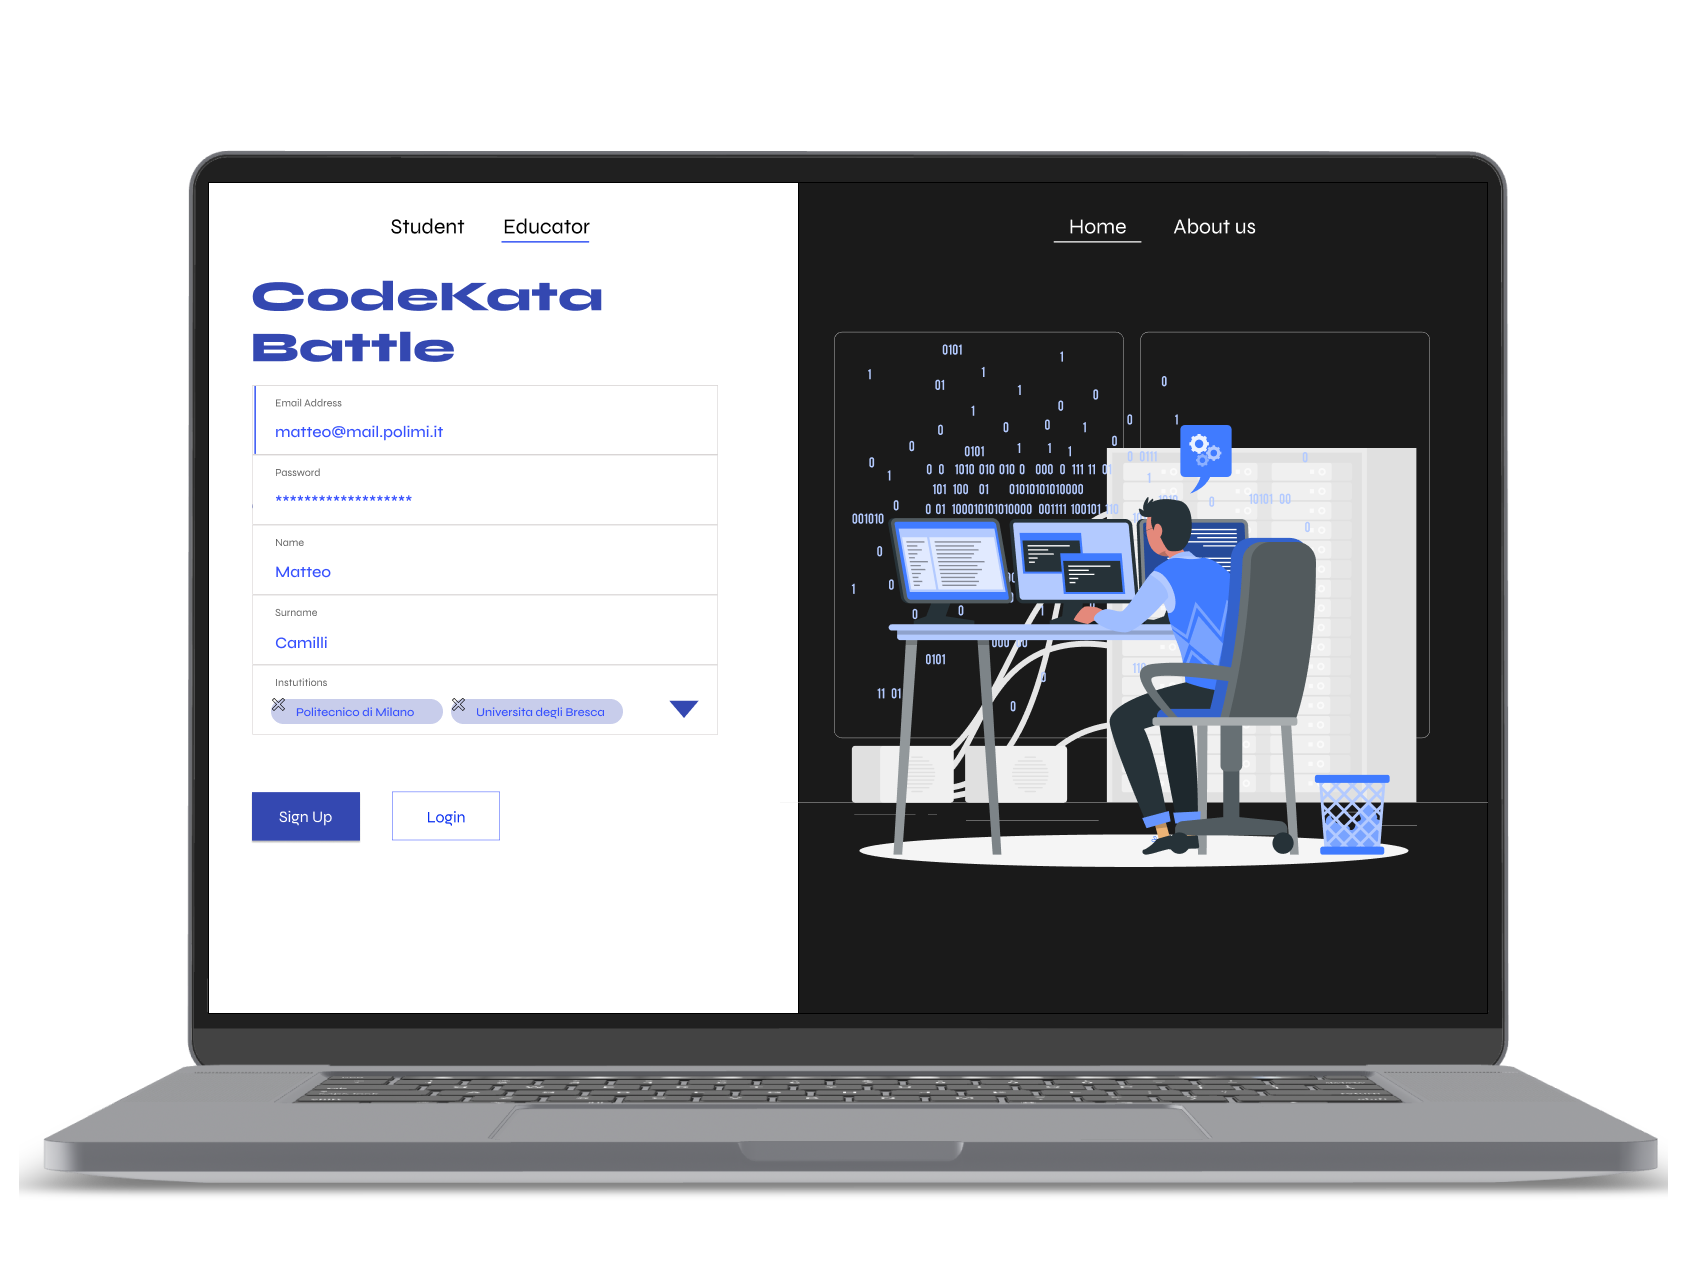
\includegraphics[scale=0.13]{Images/ui-ux/educator_signup.png}
    (a) $UI_{1}$ Sign up Screens 
\end{center}

\begin{center}
    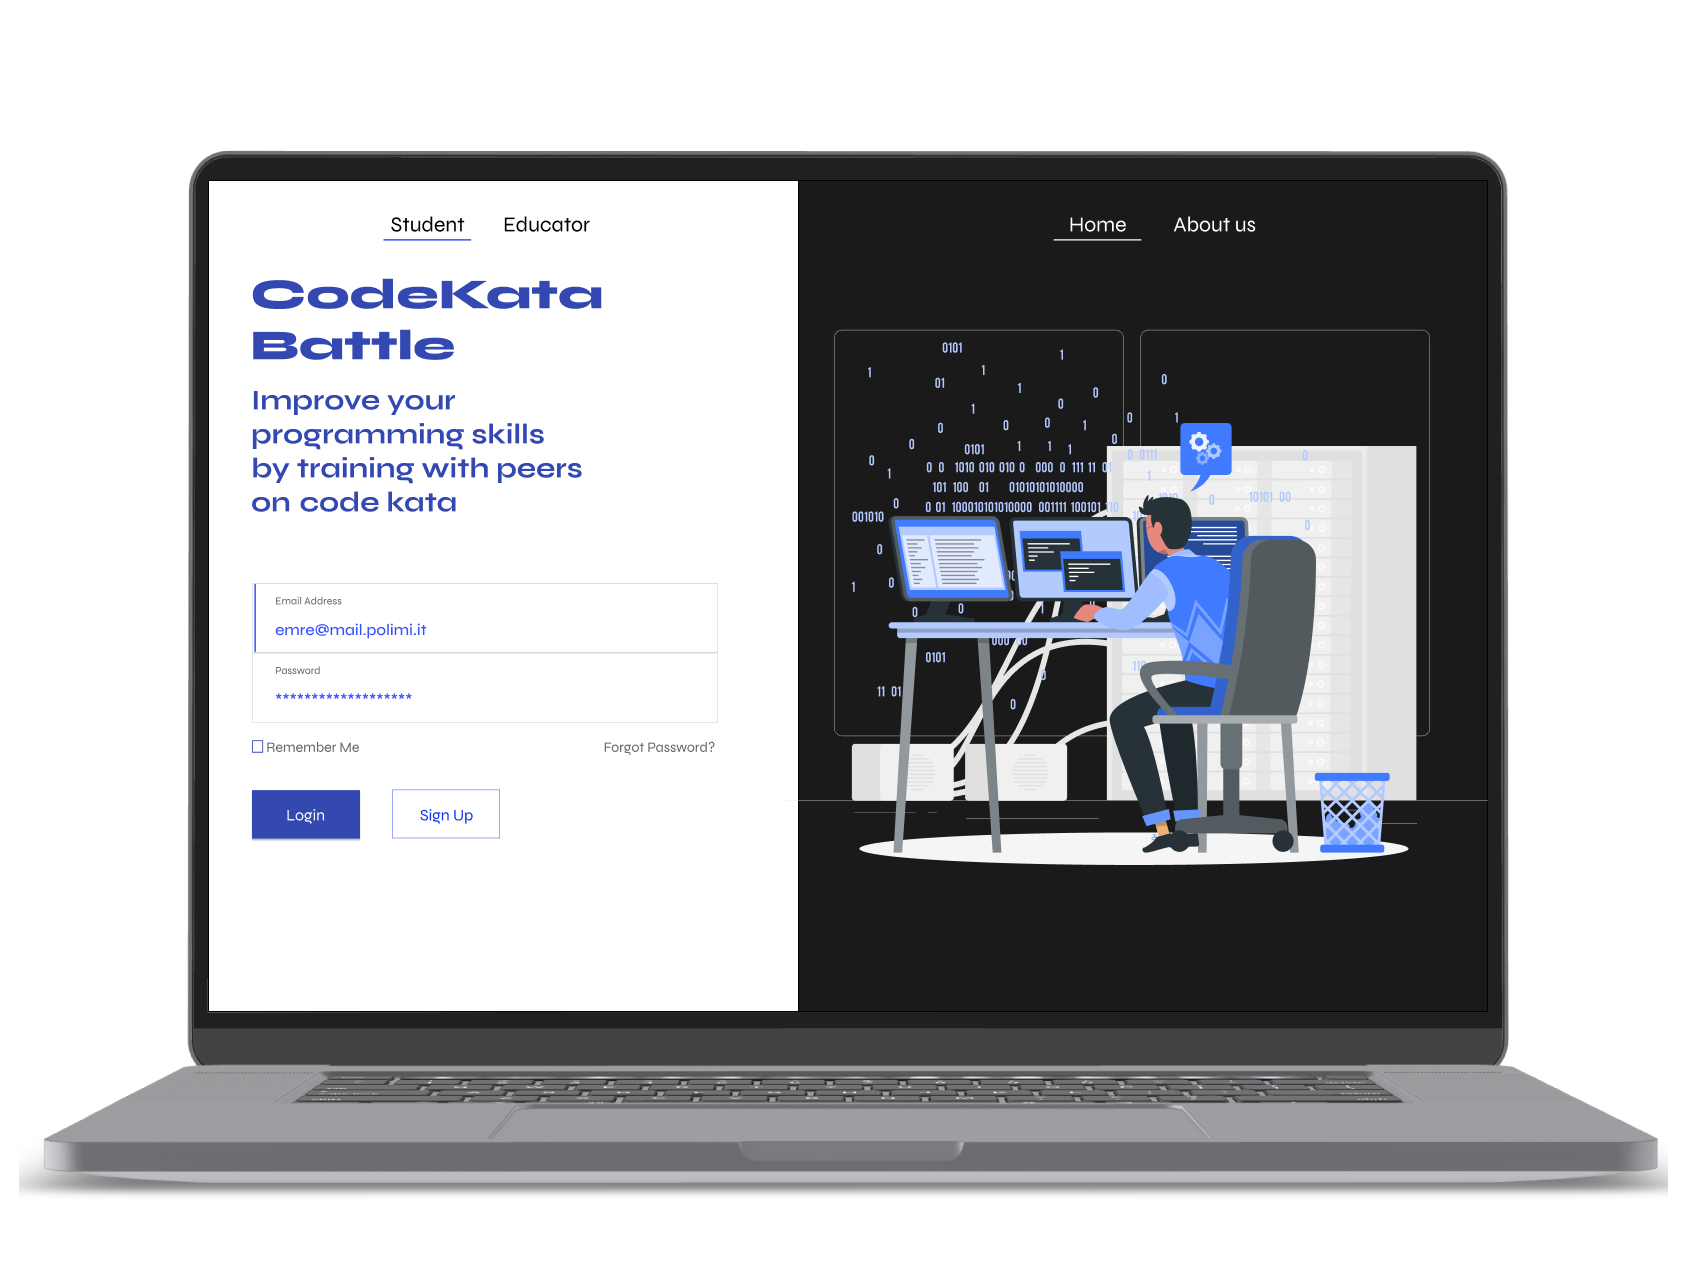
\includegraphics[scale=0.13]{Images/ui-ux/student_login.png}
    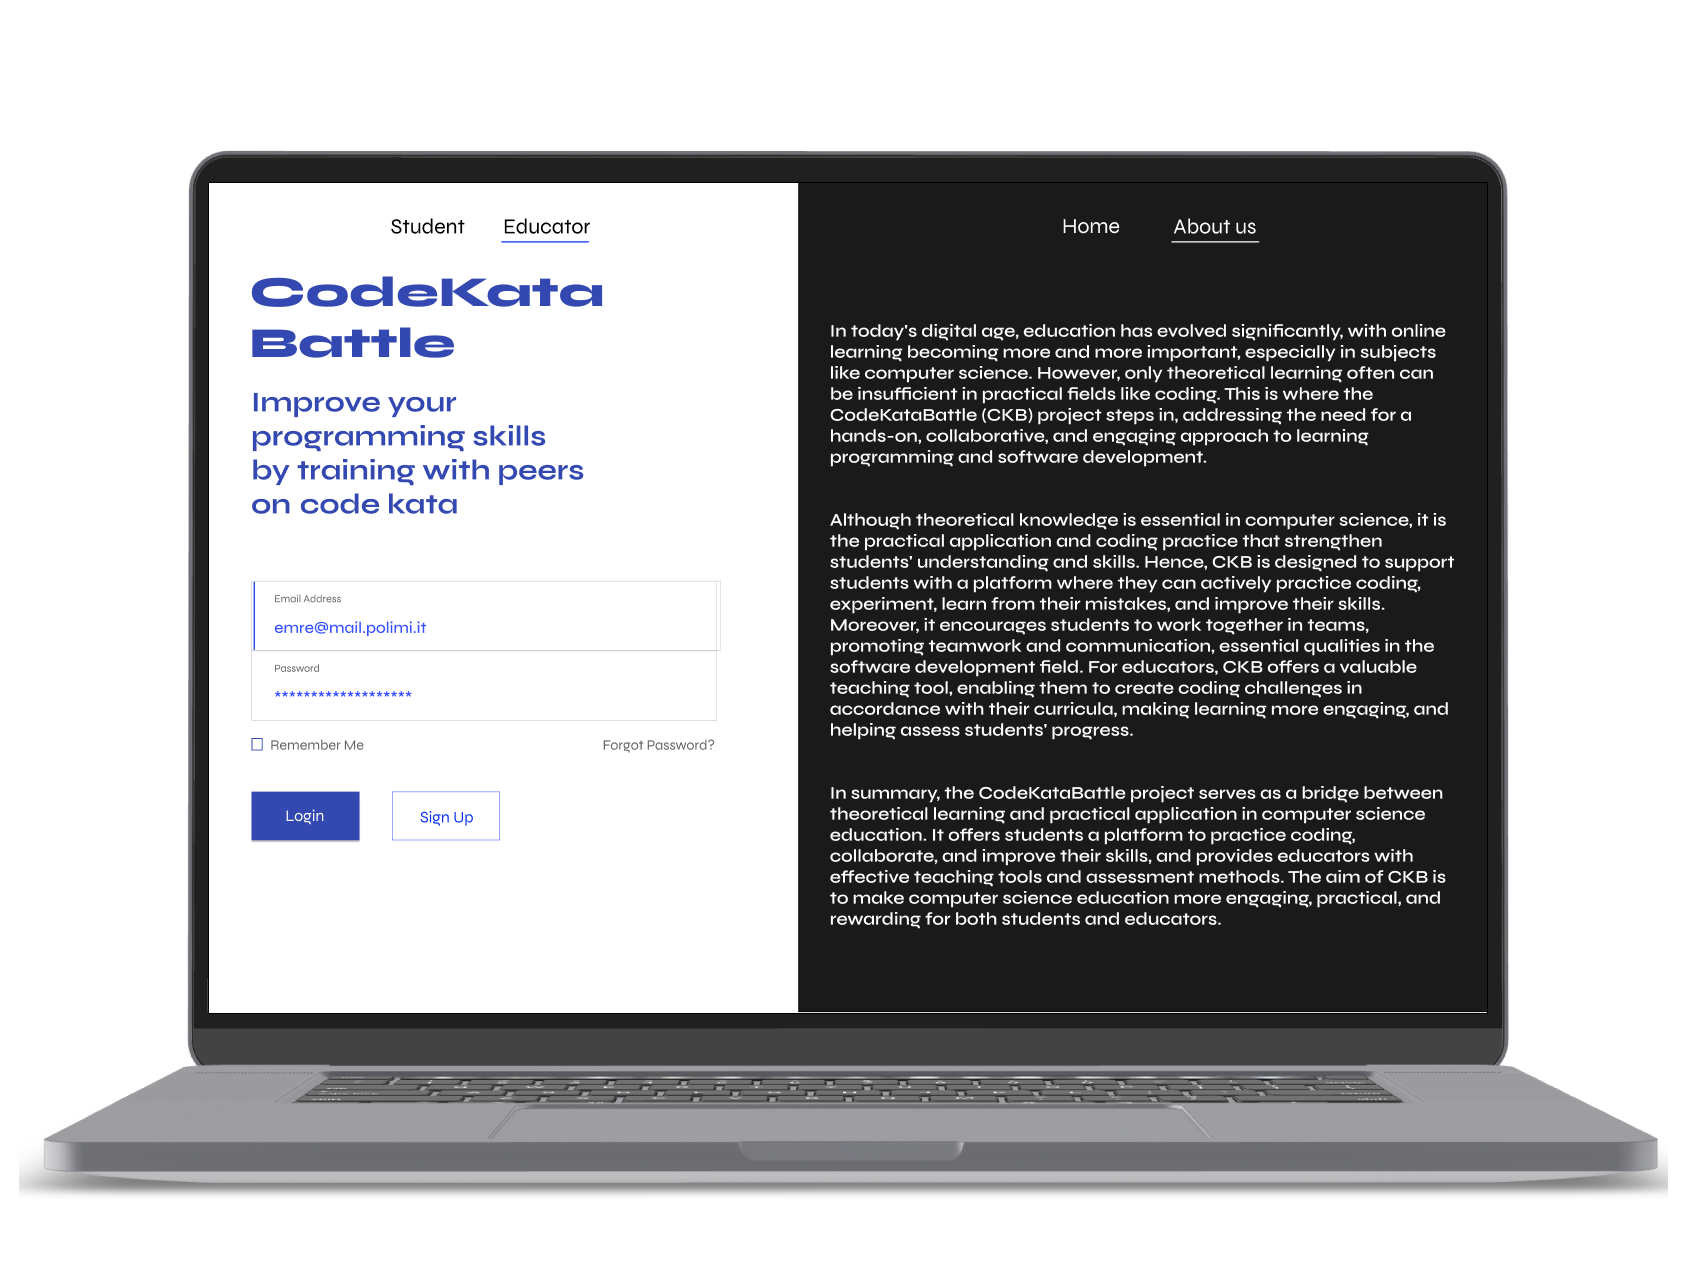
\includegraphics[scale=0.13]{Images/ui-ux/educator_login.png}
\end{center}
    \begin{center}
        (b) $UI_{2}$ Login Screens
    \end{center}

\newpage
\begin{center}
    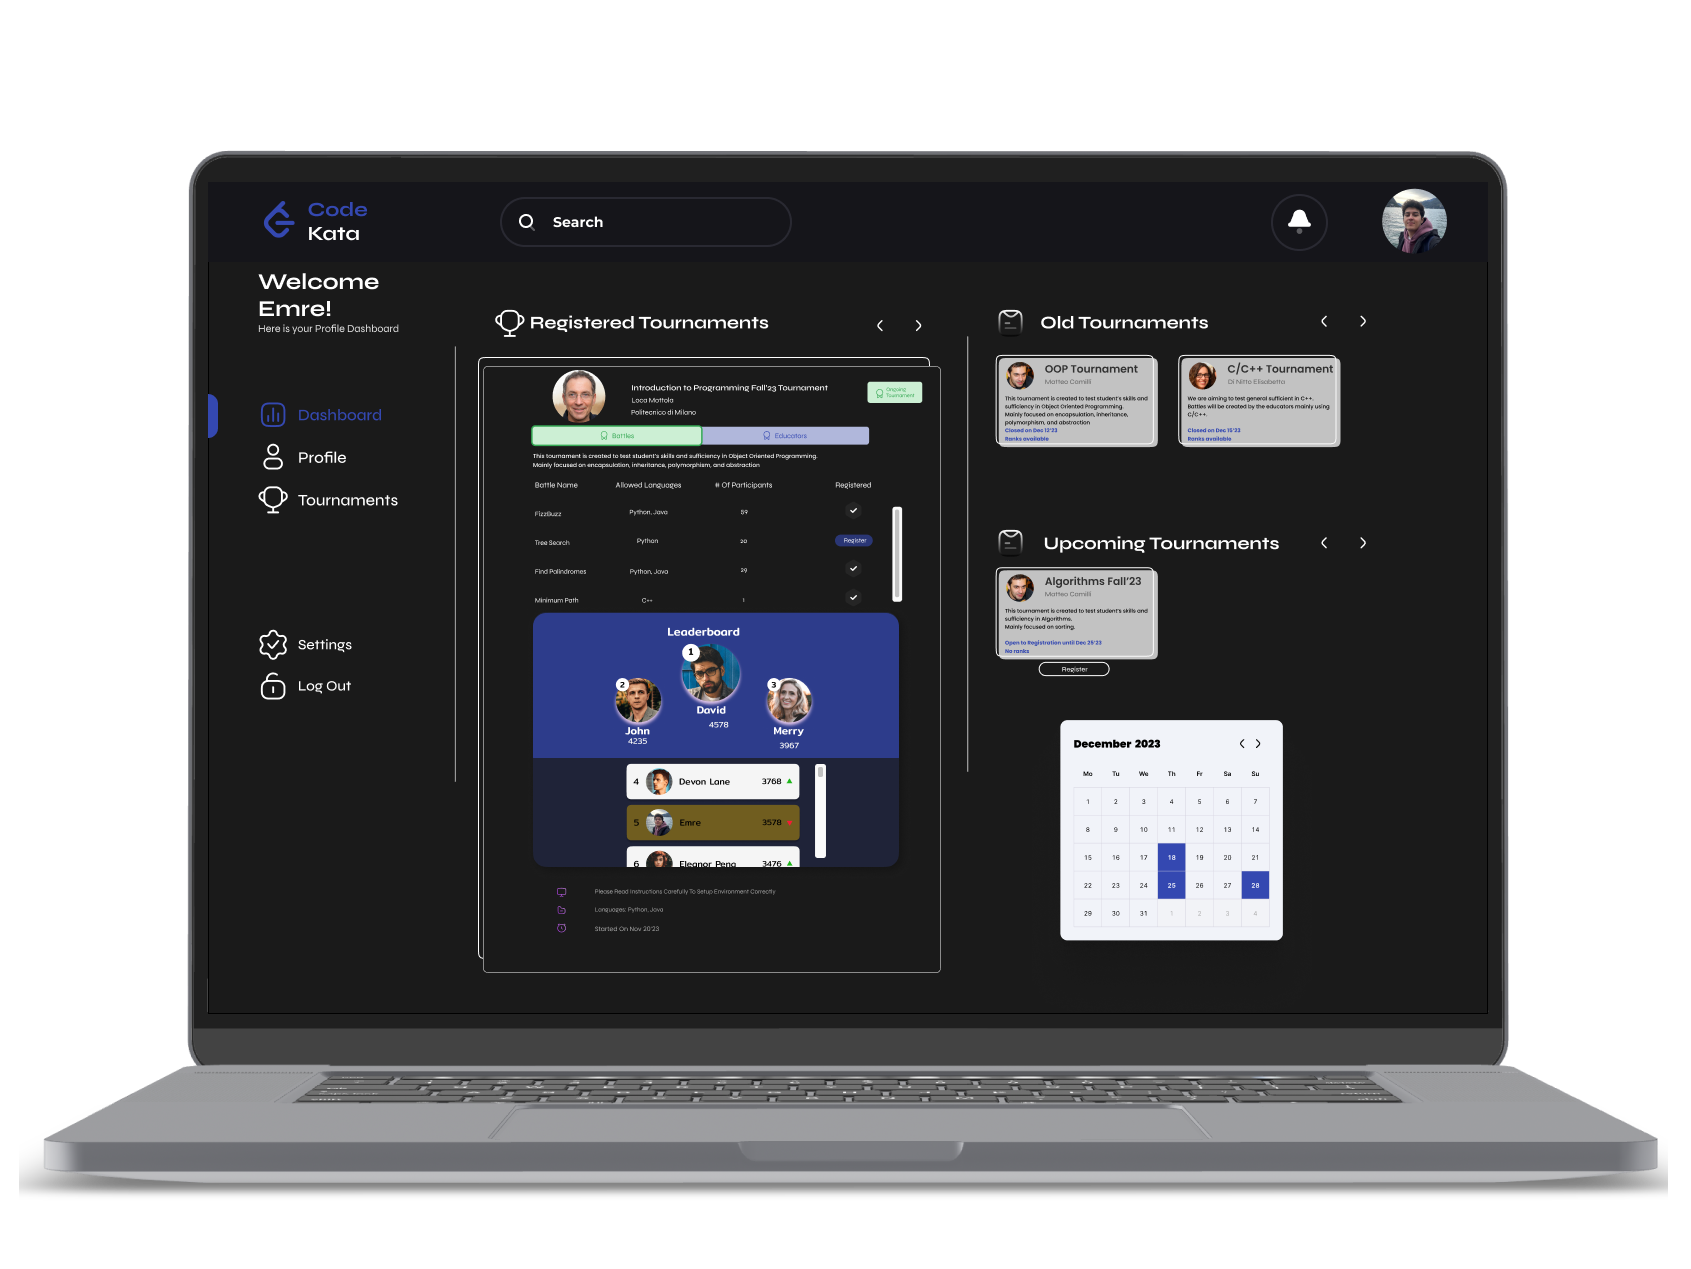
\includegraphics[scale=0.13]{Images/ui-ux/student_dashboard_1.png}
    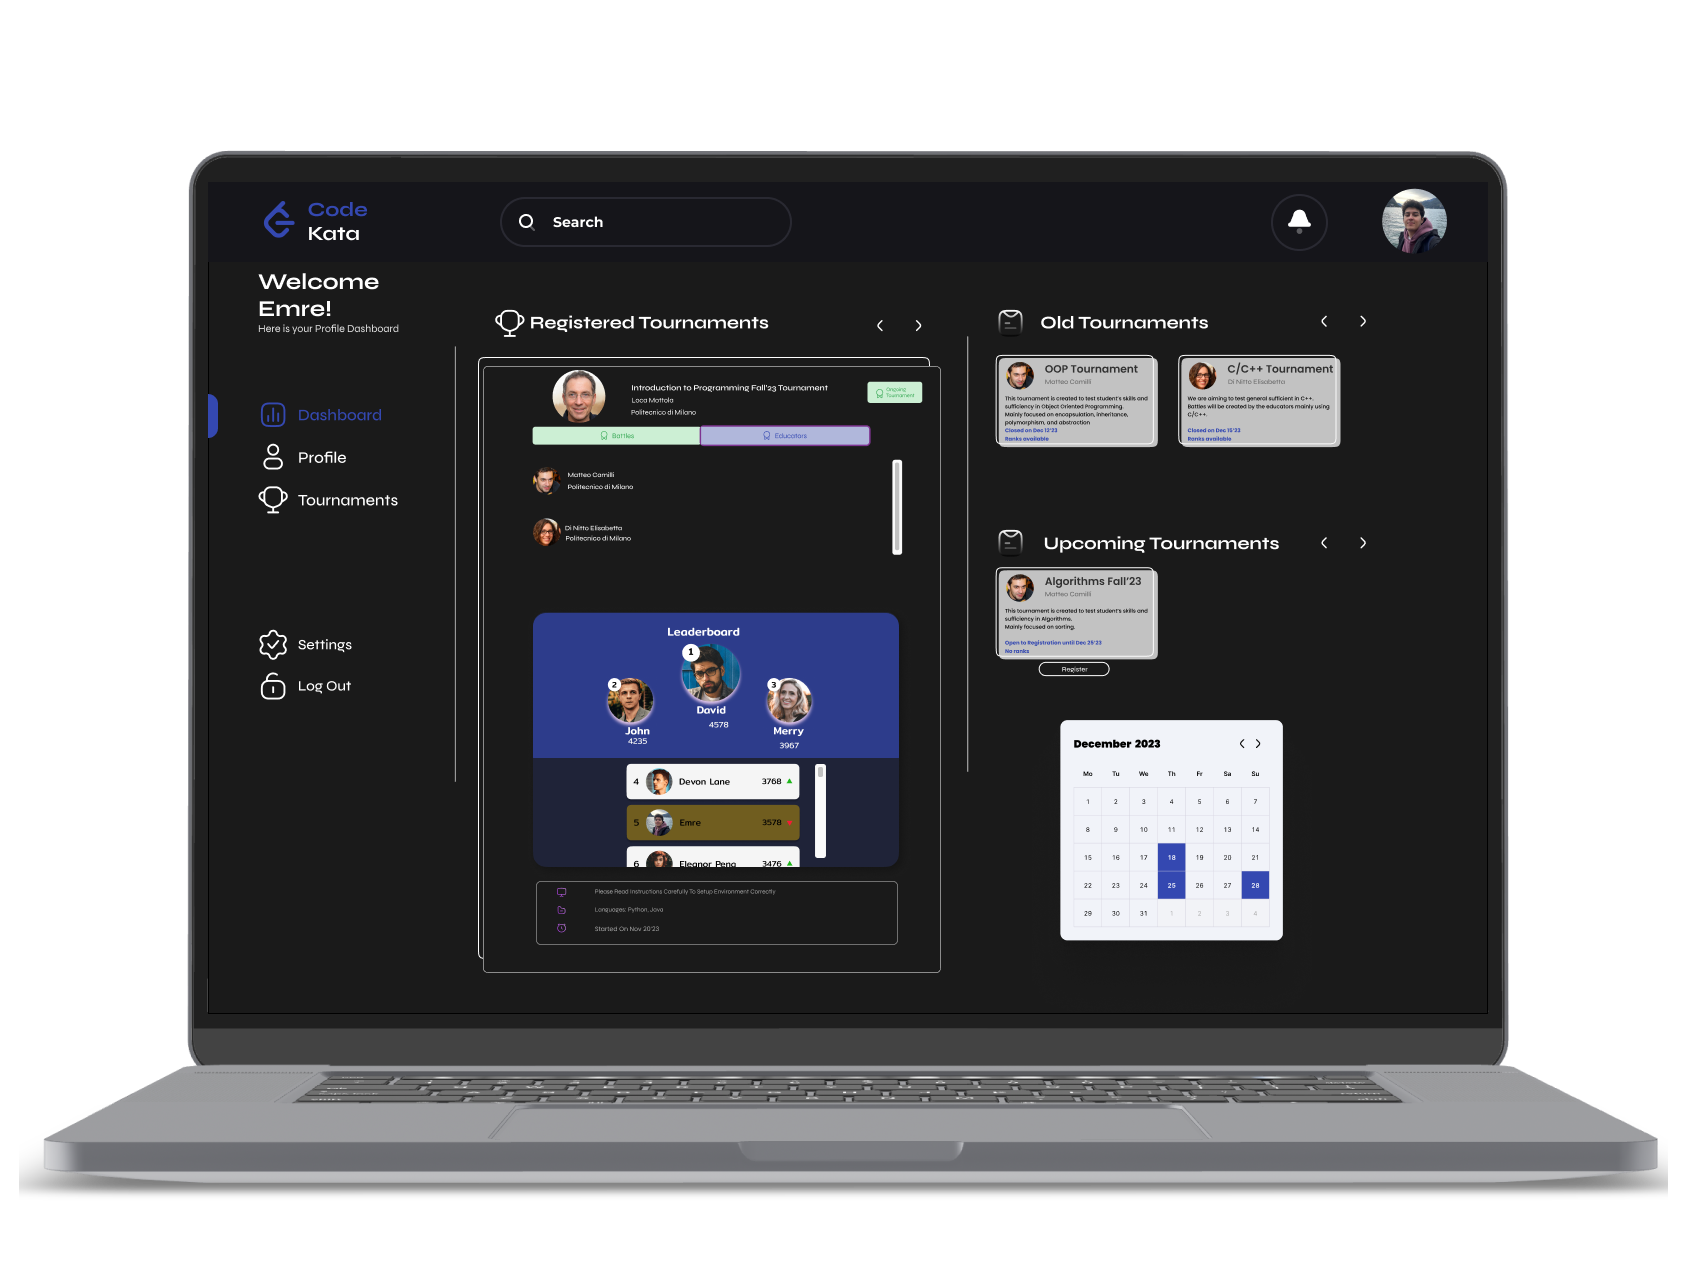
\includegraphics[scale=0.13]{Images/ui-ux/student_dashboard_2.png}
        (c) $UI_{3}$ Student Dashboard
\end{center}
\begin{center}
    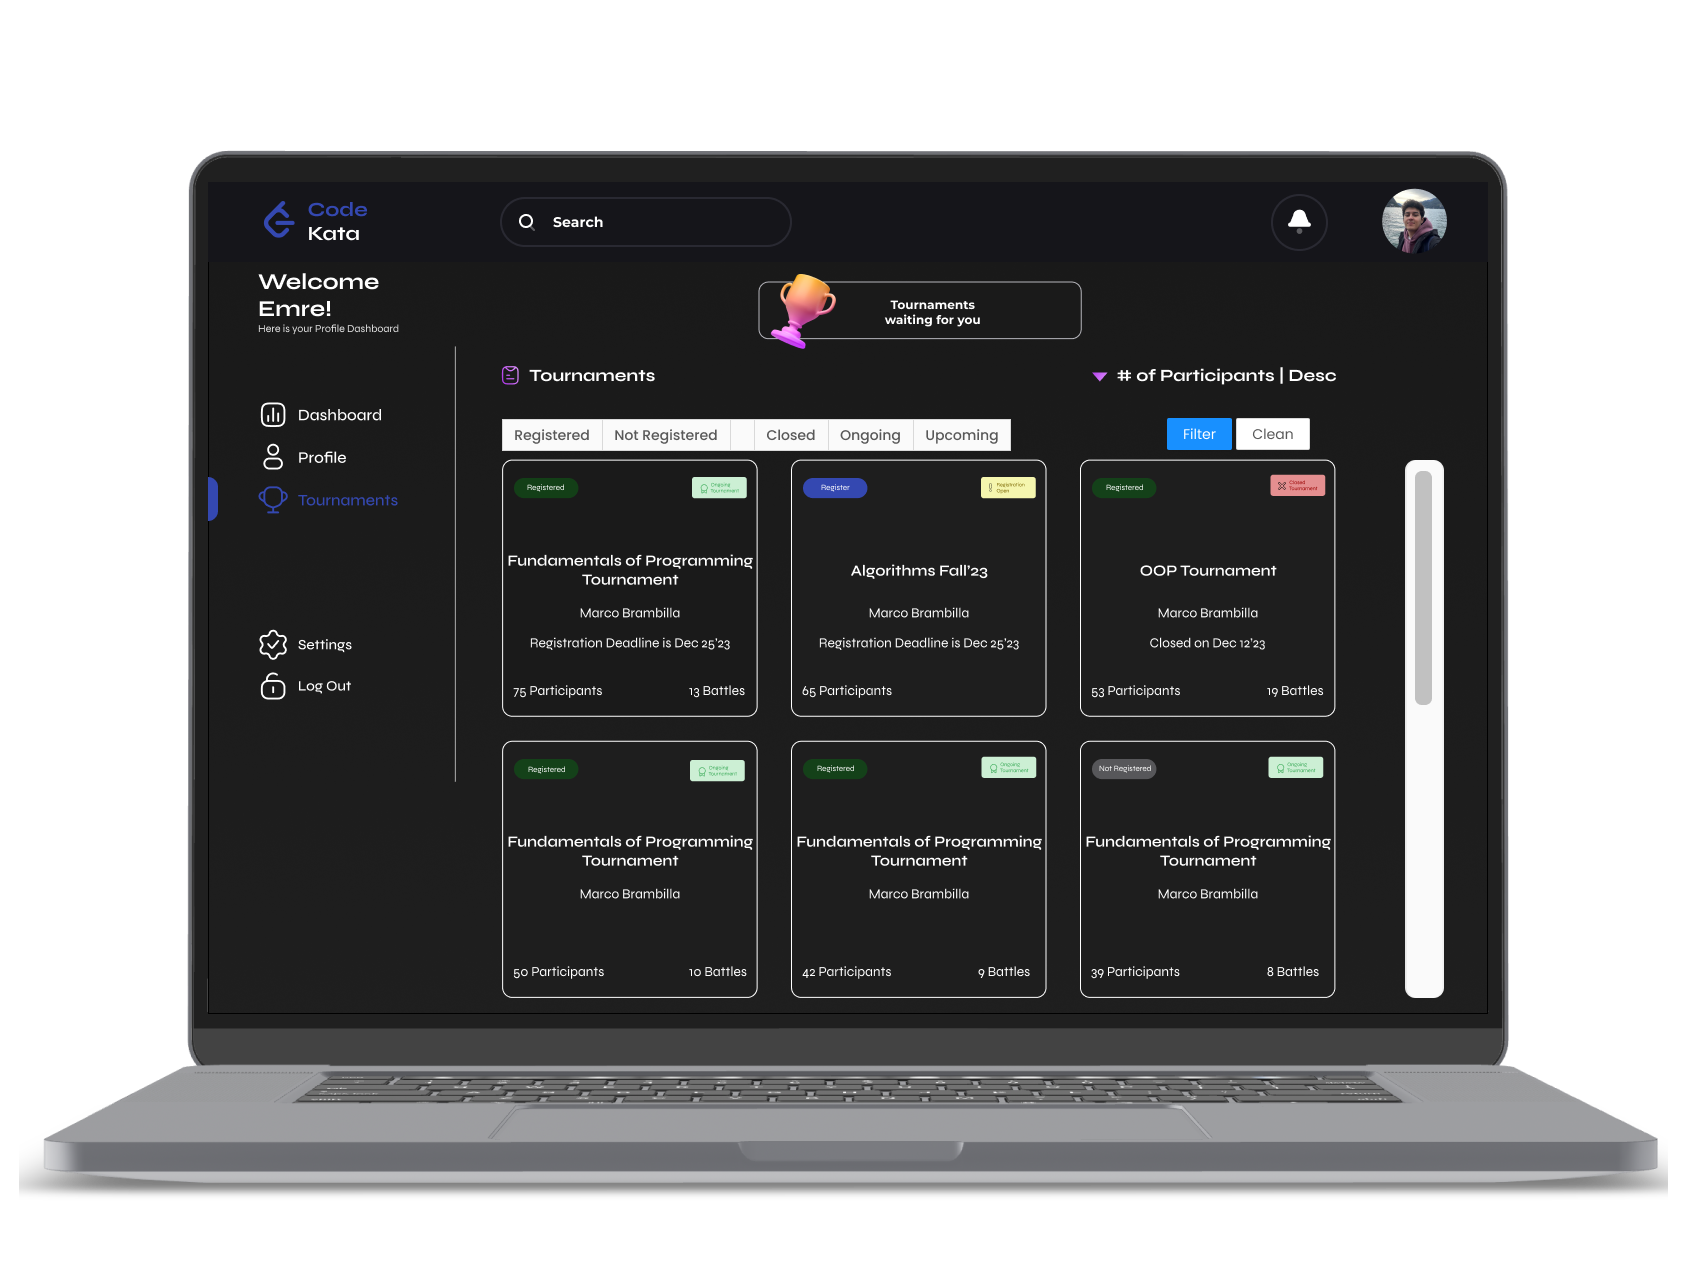
\includegraphics[scale=0.13]{Images/ui-ux/student_tournaments_1.png}
    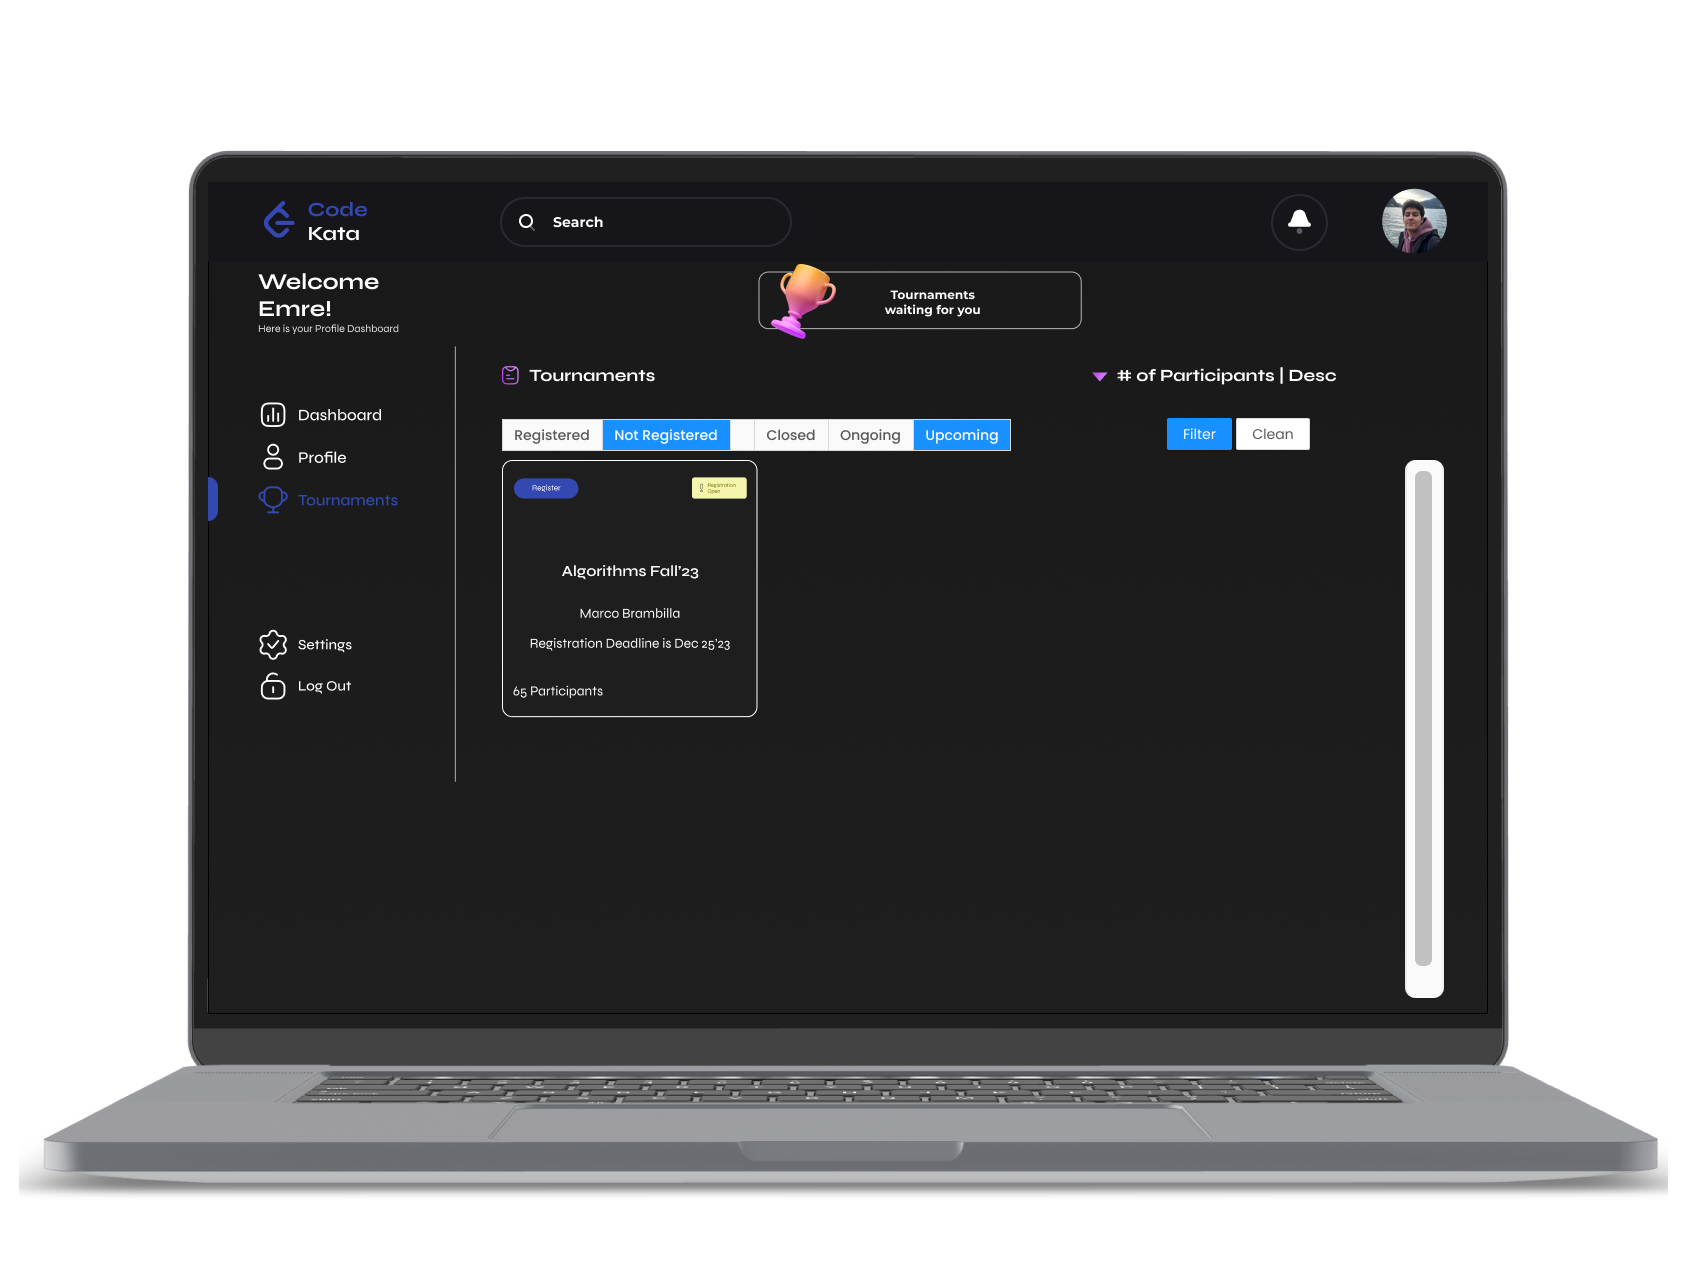
\includegraphics[scale=0.13]{Images/ui-ux/student_tournaments_2.png}    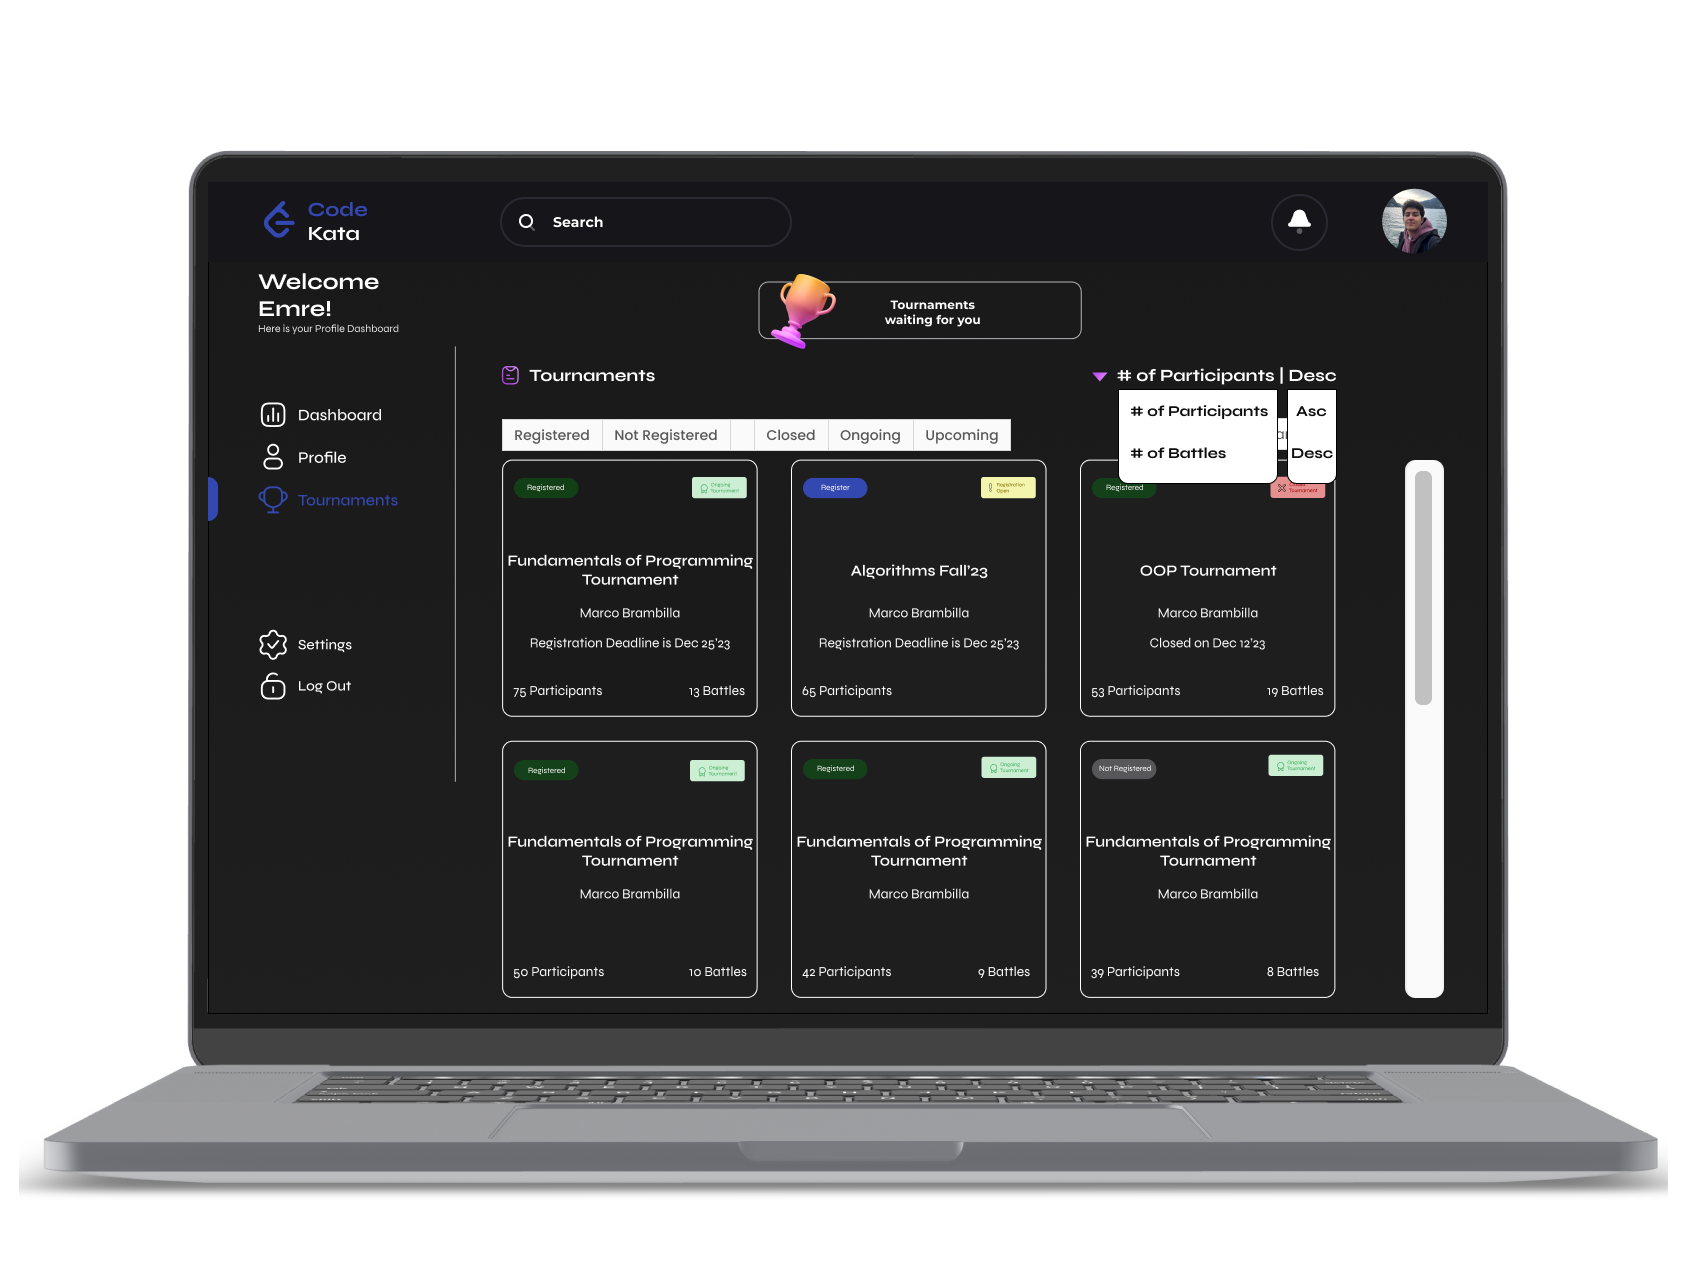
\includegraphics[scale=0.13]{Images/ui-ux/student_tournaments_3.png}    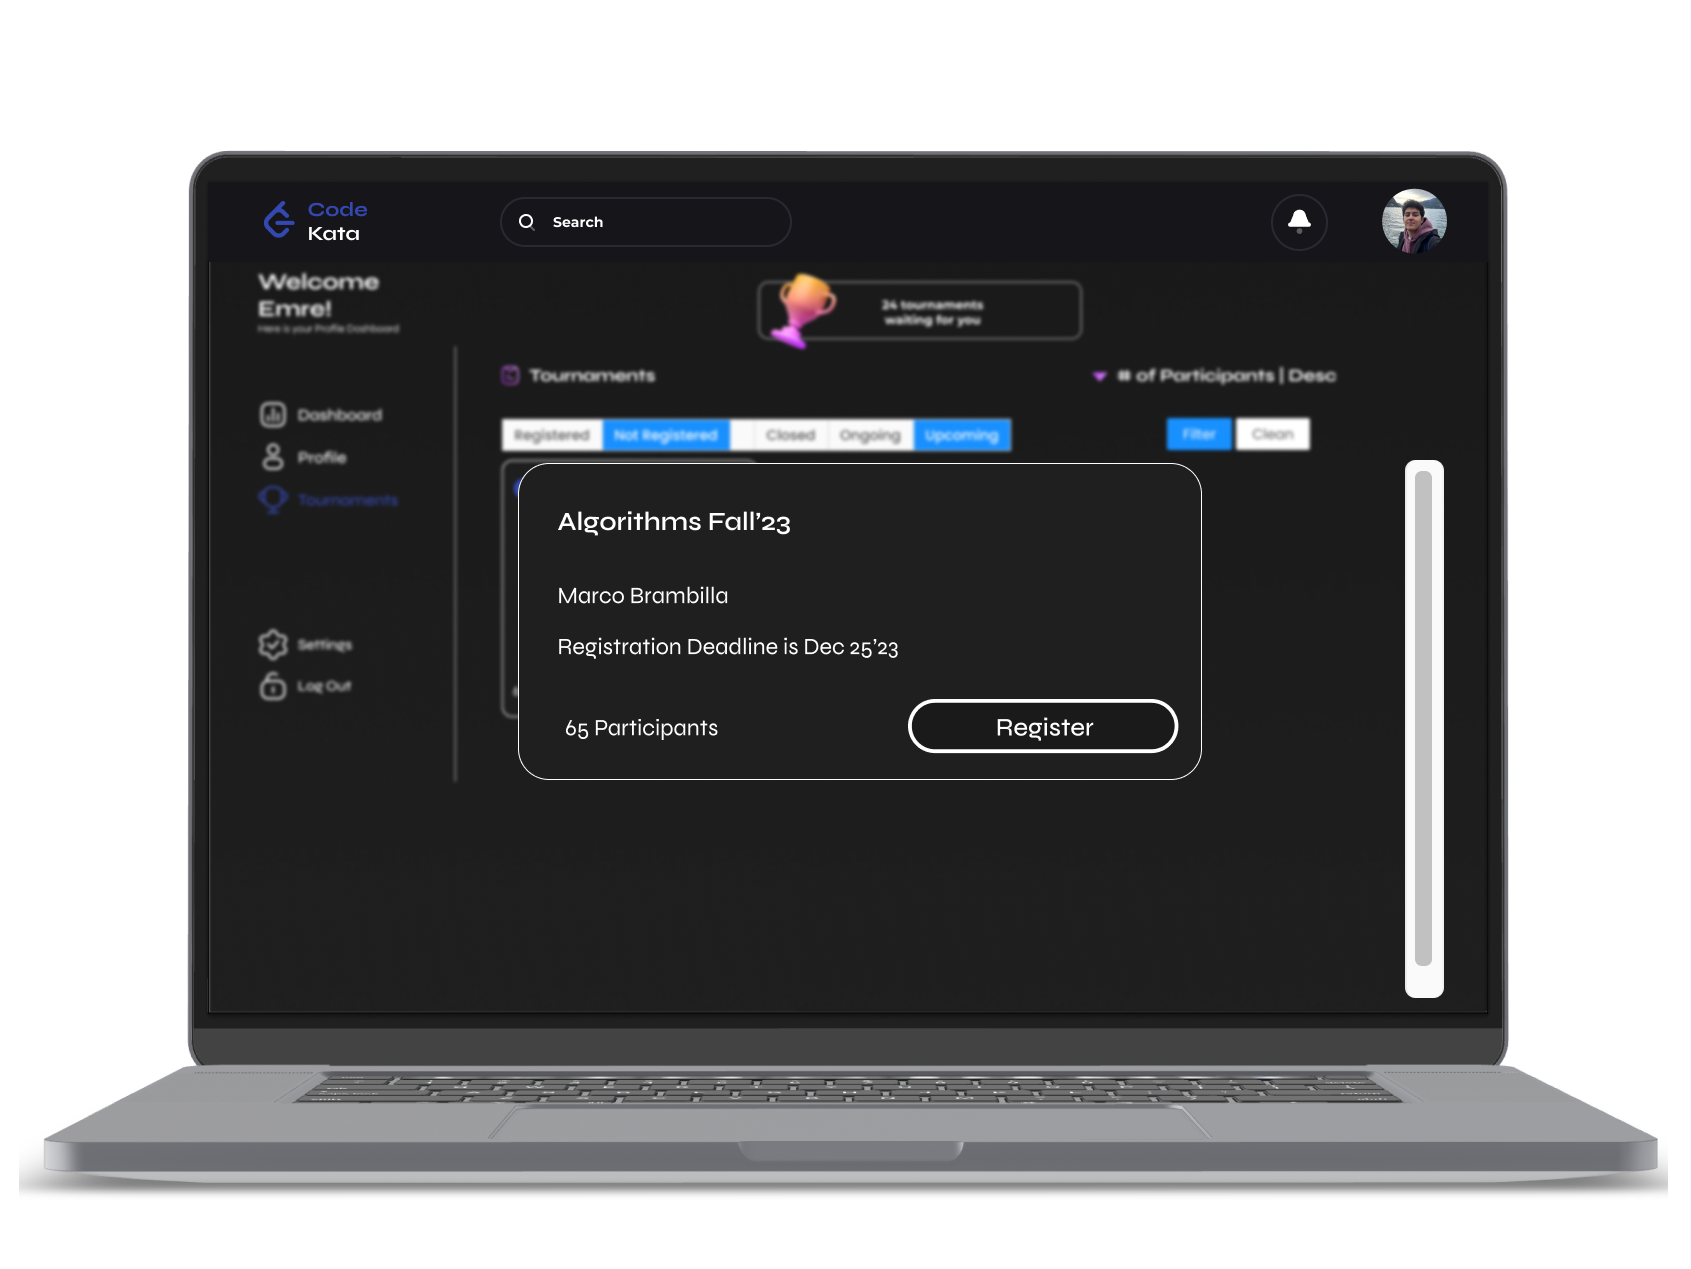
\includegraphics[scale=0.13]{Images/ui-ux/student_tournaments_4.png}
        (d) $UI_{4}$ Student Tournaments Page
\end{center}

\begin{center}
    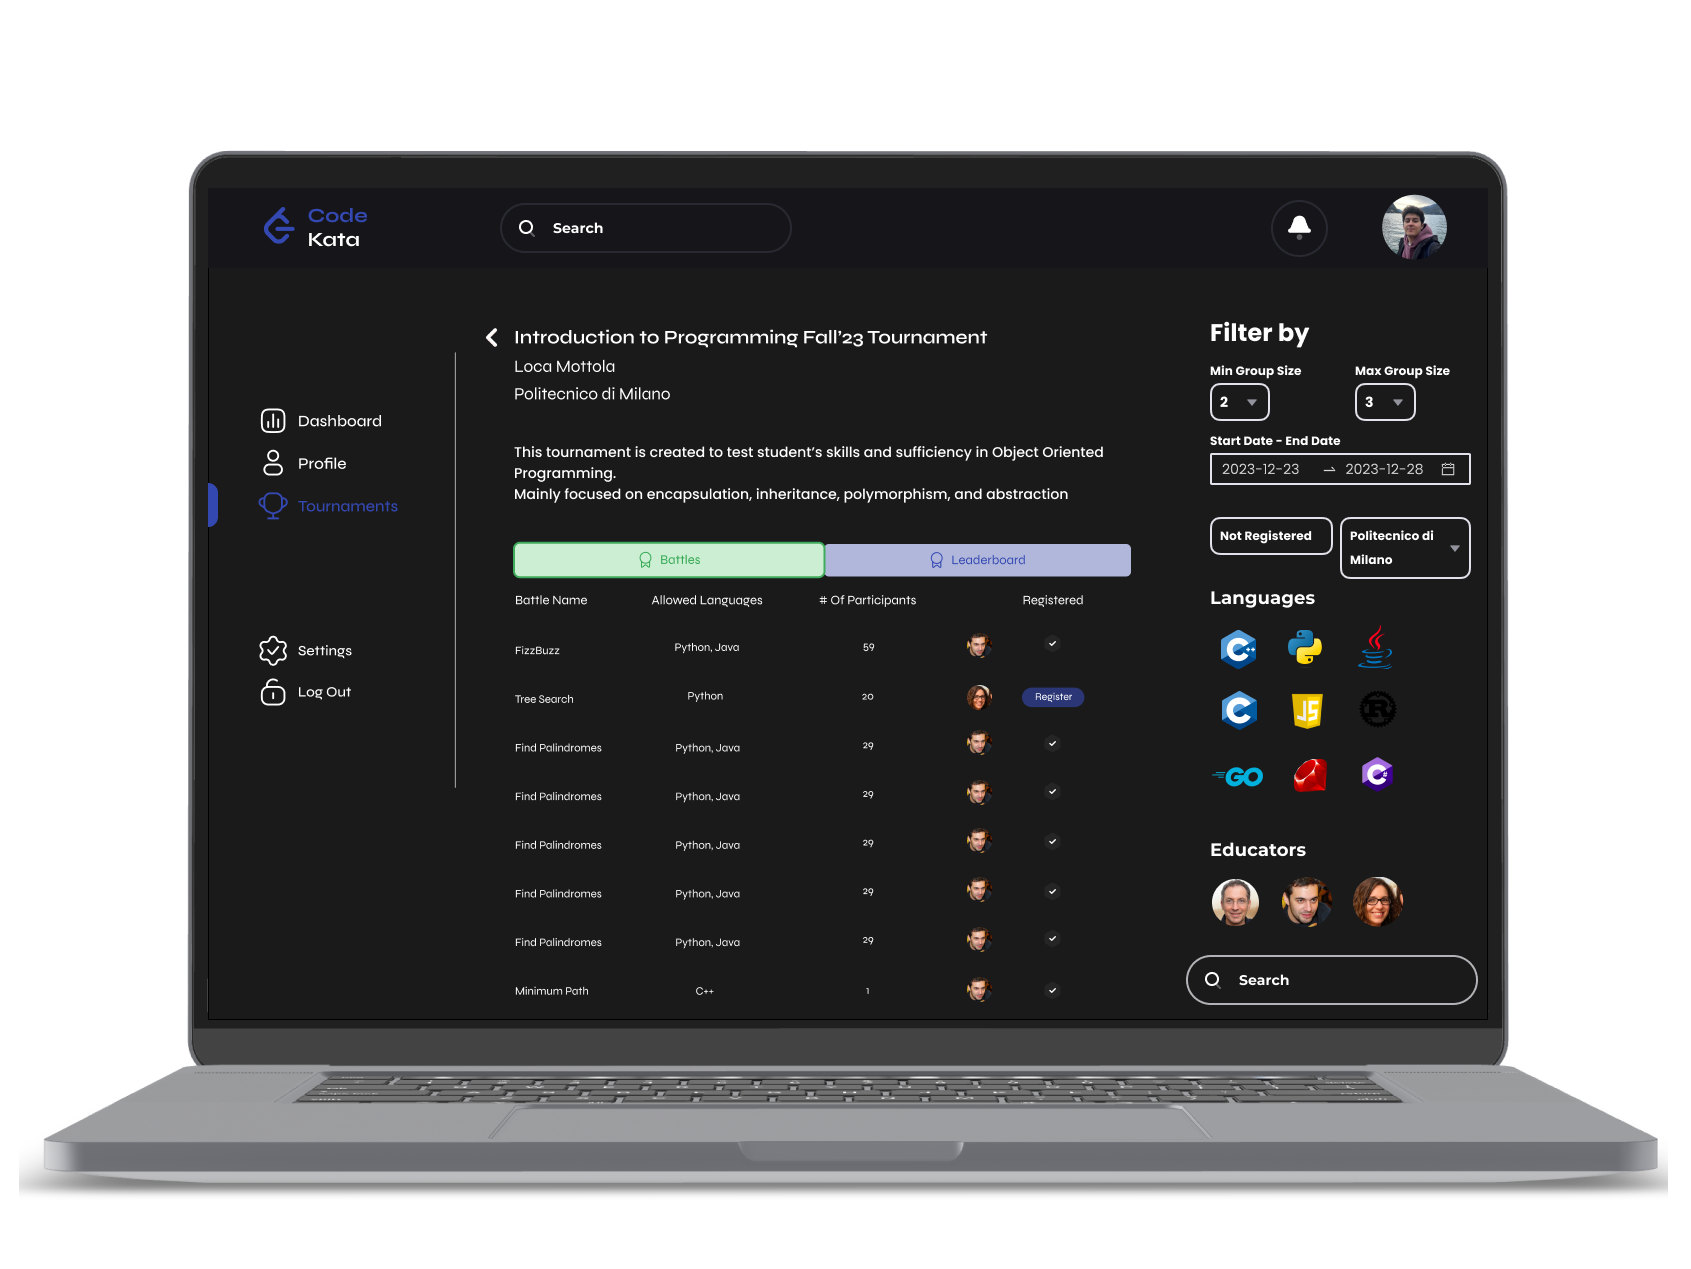
\includegraphics[scale=0.13]{Images/ui-ux/student_tournament_1.png}
    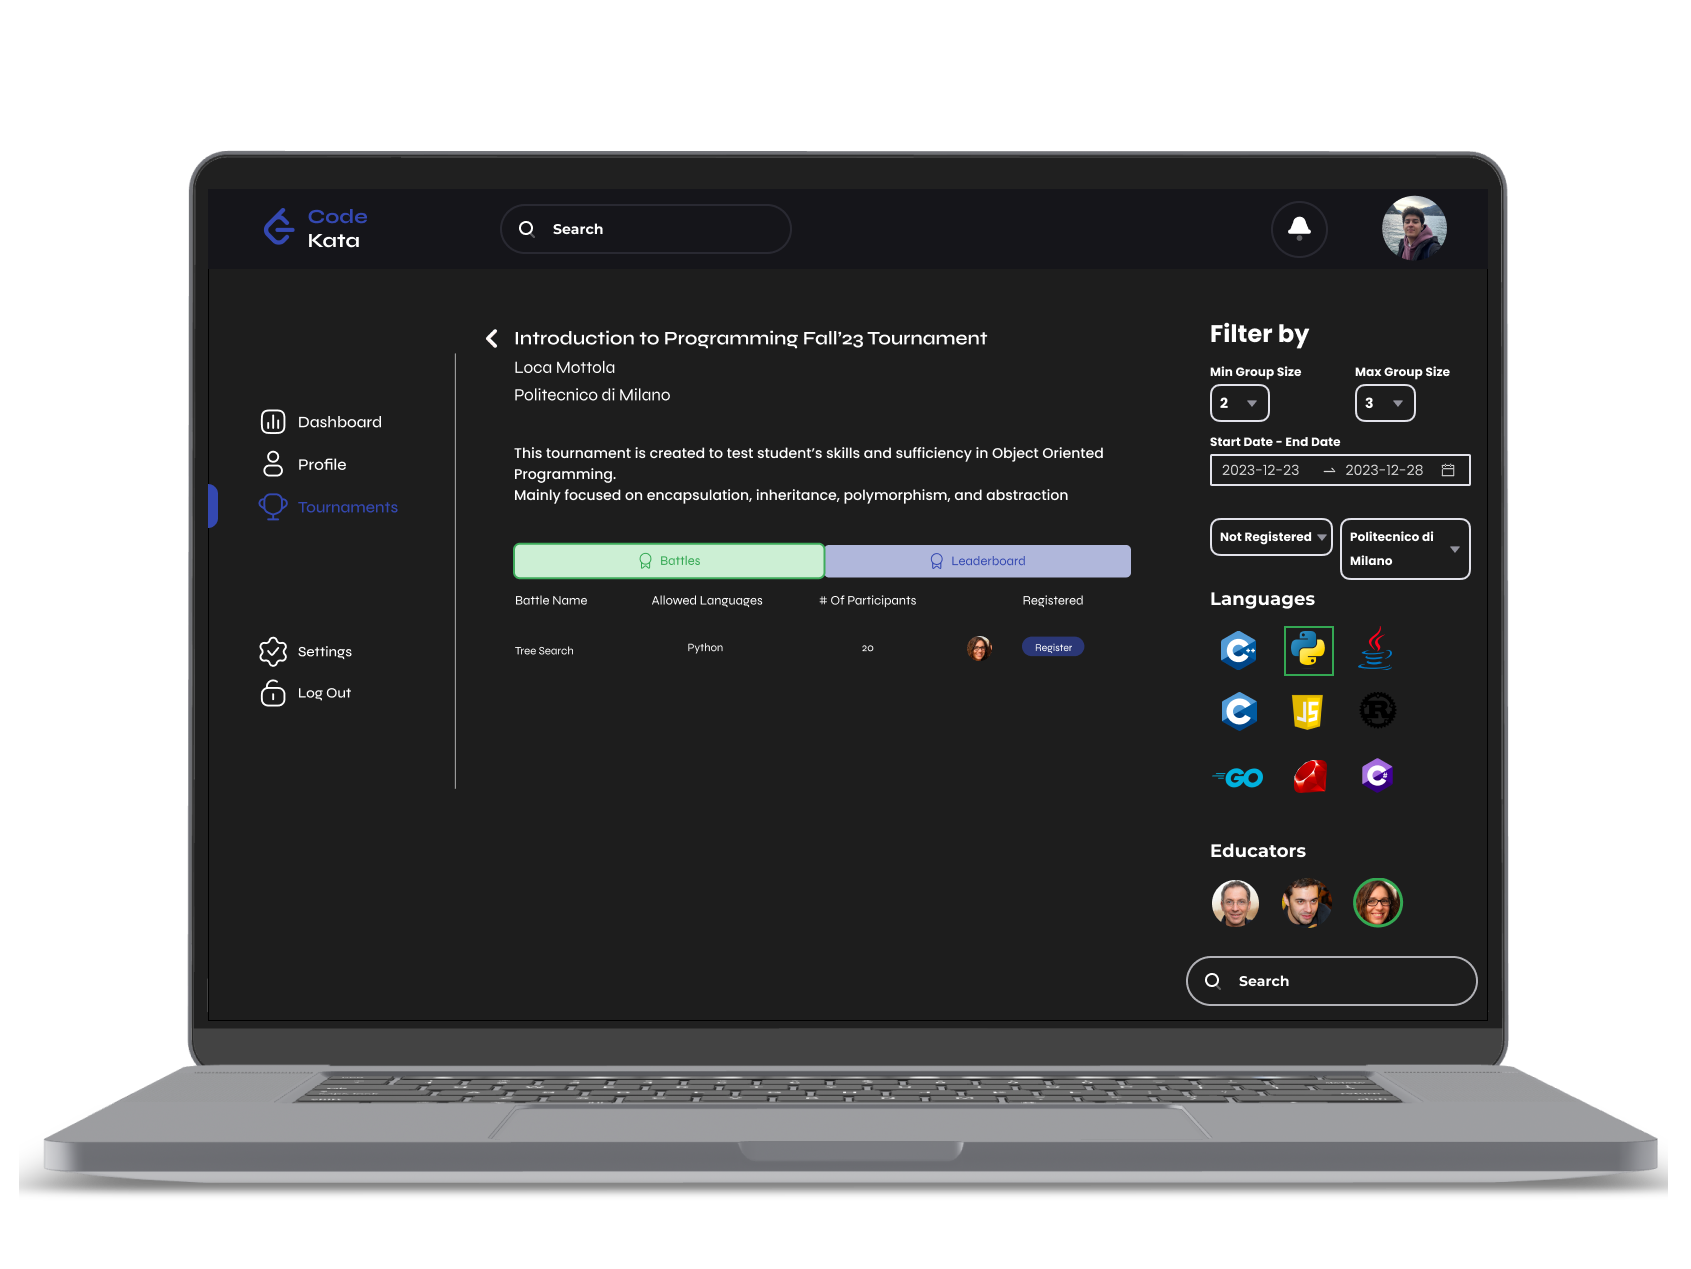
\includegraphics[scale=0.13]{Images/ui-ux/student_tournament_2.png}    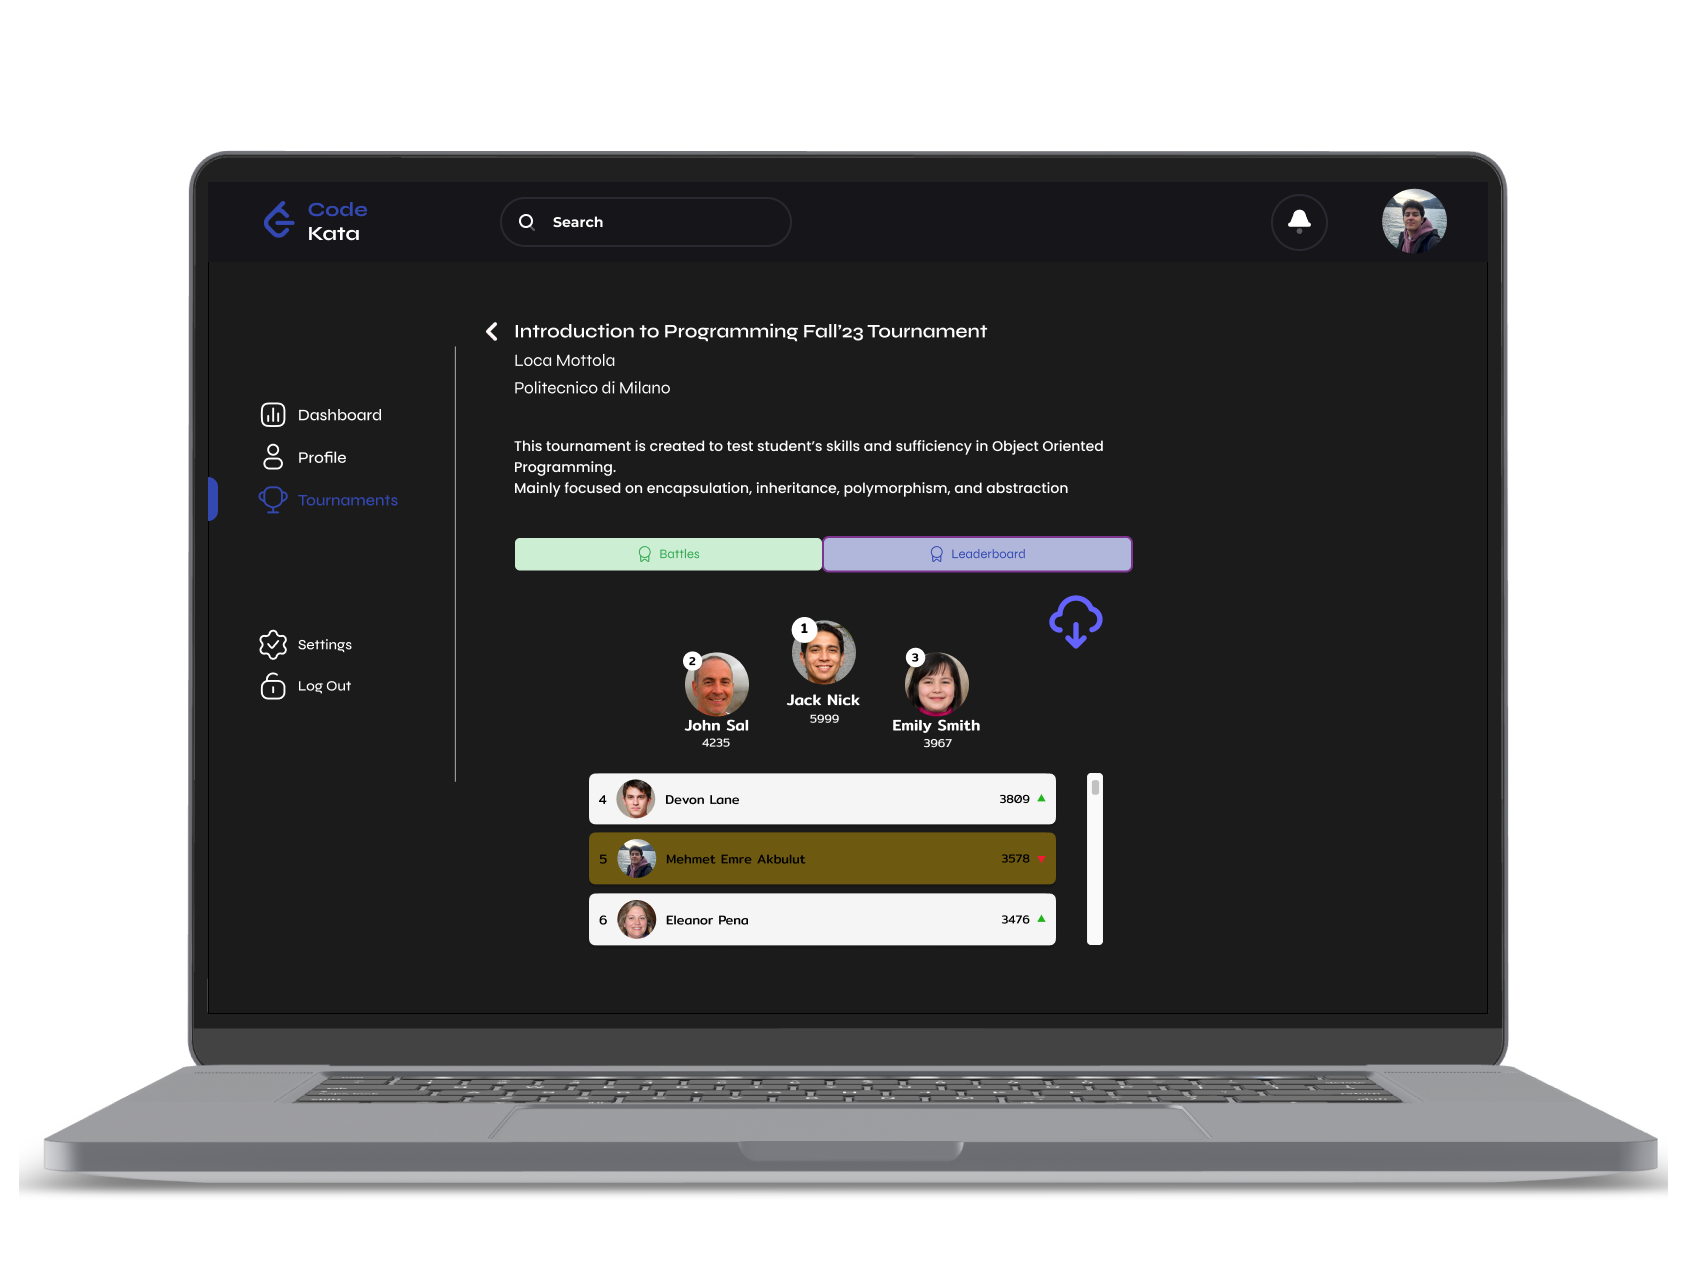
\includegraphics[scale=0.13]{Images/ui-ux/student_tournament_3.png} 
    \\ (e) $UI_{5}$ Student visits a Tournament 
\end{center}
\newpage
\begin{center}
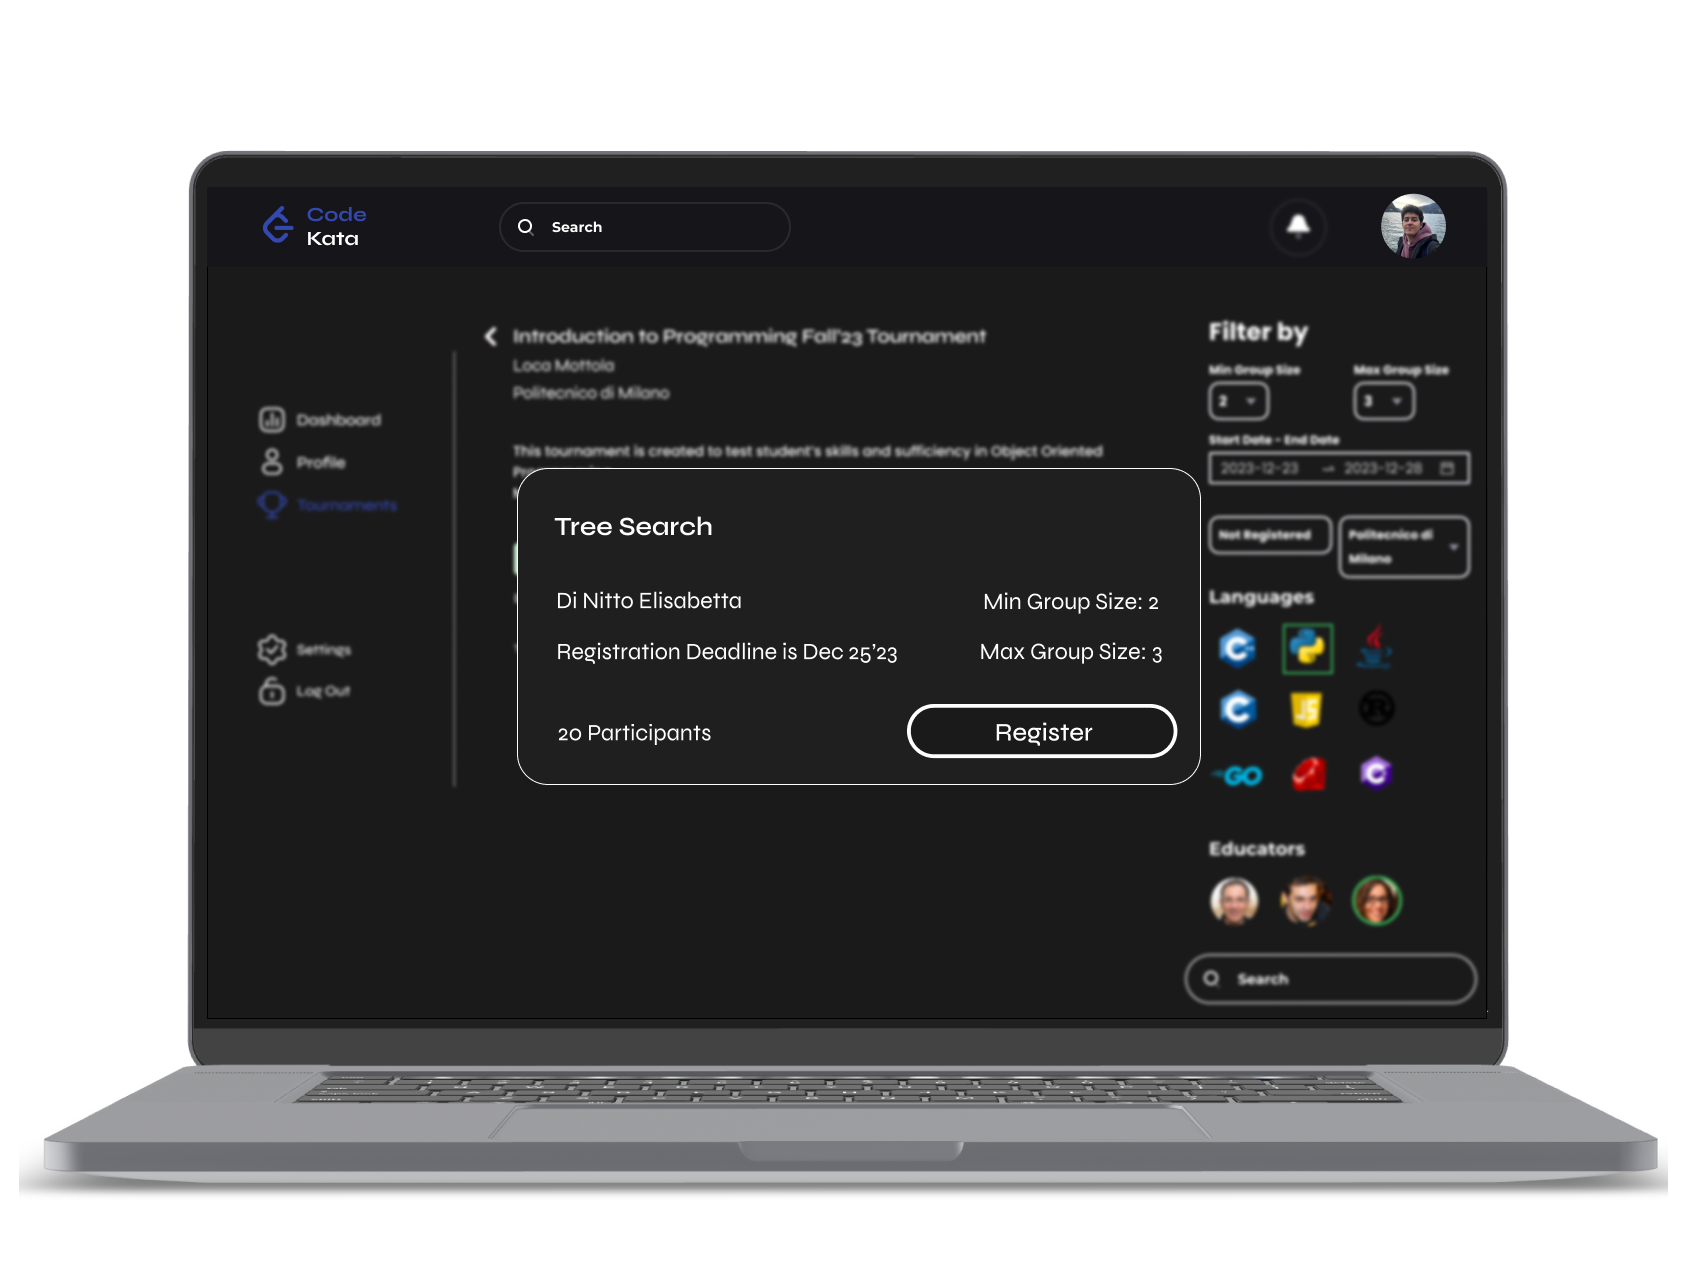
\includegraphics[scale=0.13]{Images/ui-ux/student_battle_register_1.png}
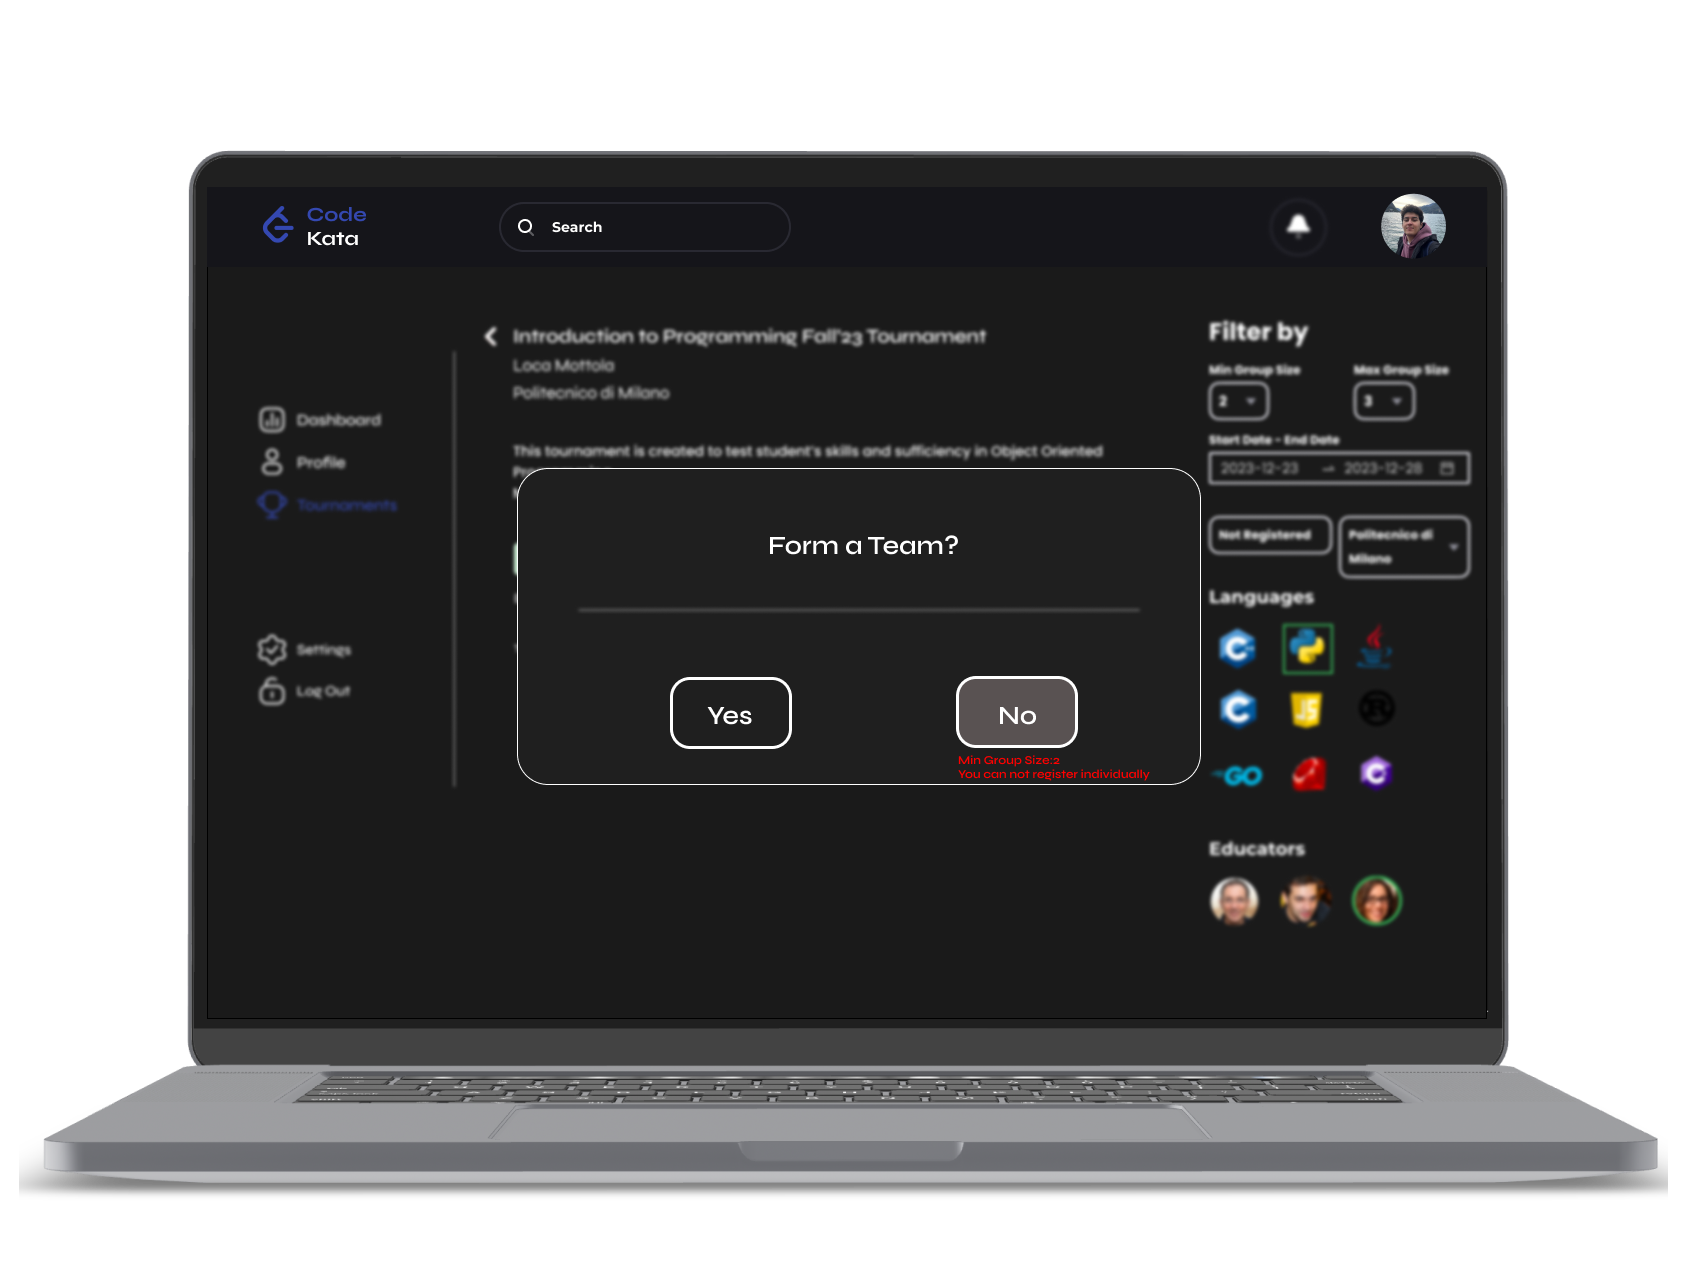
\includegraphics[scale=0.13]{Images/ui-ux/student_battle_register_2.png}
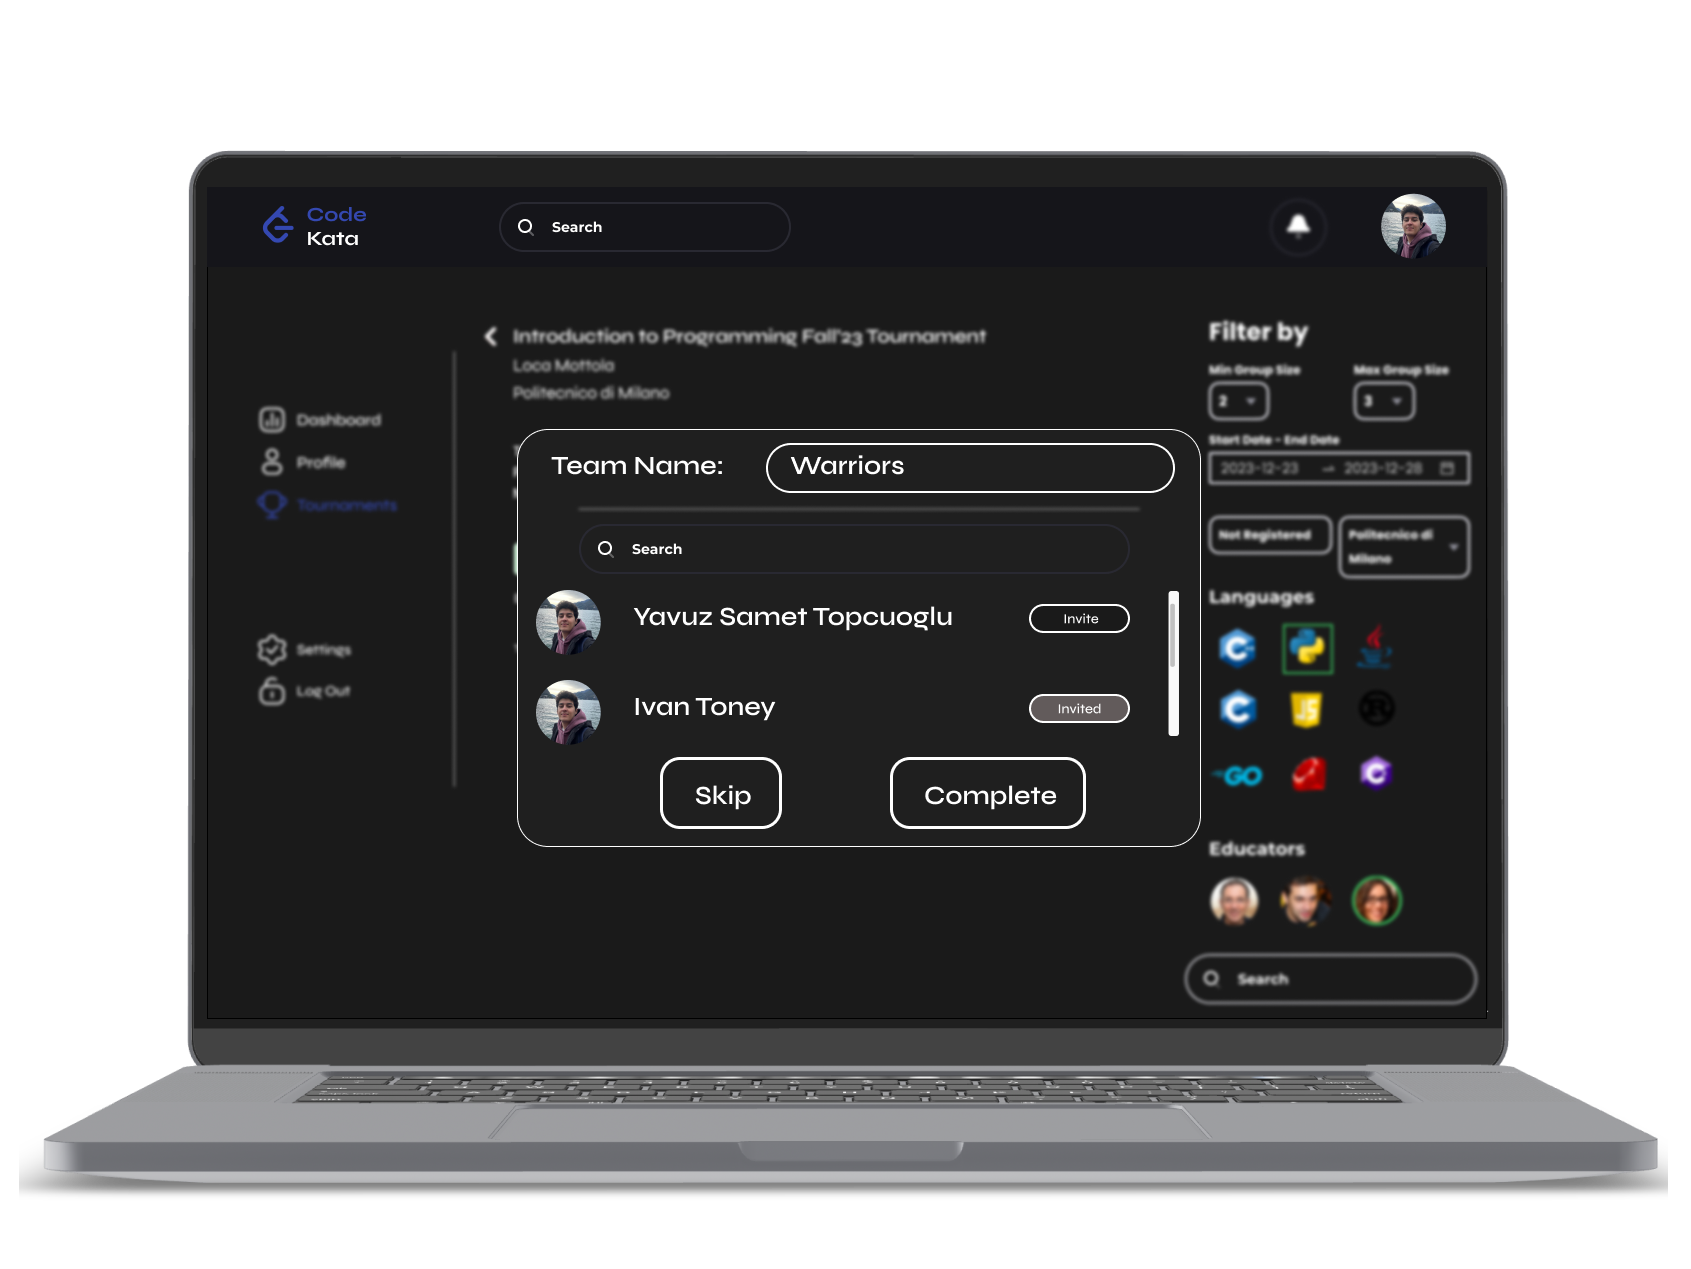
\includegraphics[scale=0.13]{Images/ui-ux/student_battle_register_3.png}
\\ (f) $UI_{6}$  Student Registers Battle 
\end{center}
\newpage
\begin{center}
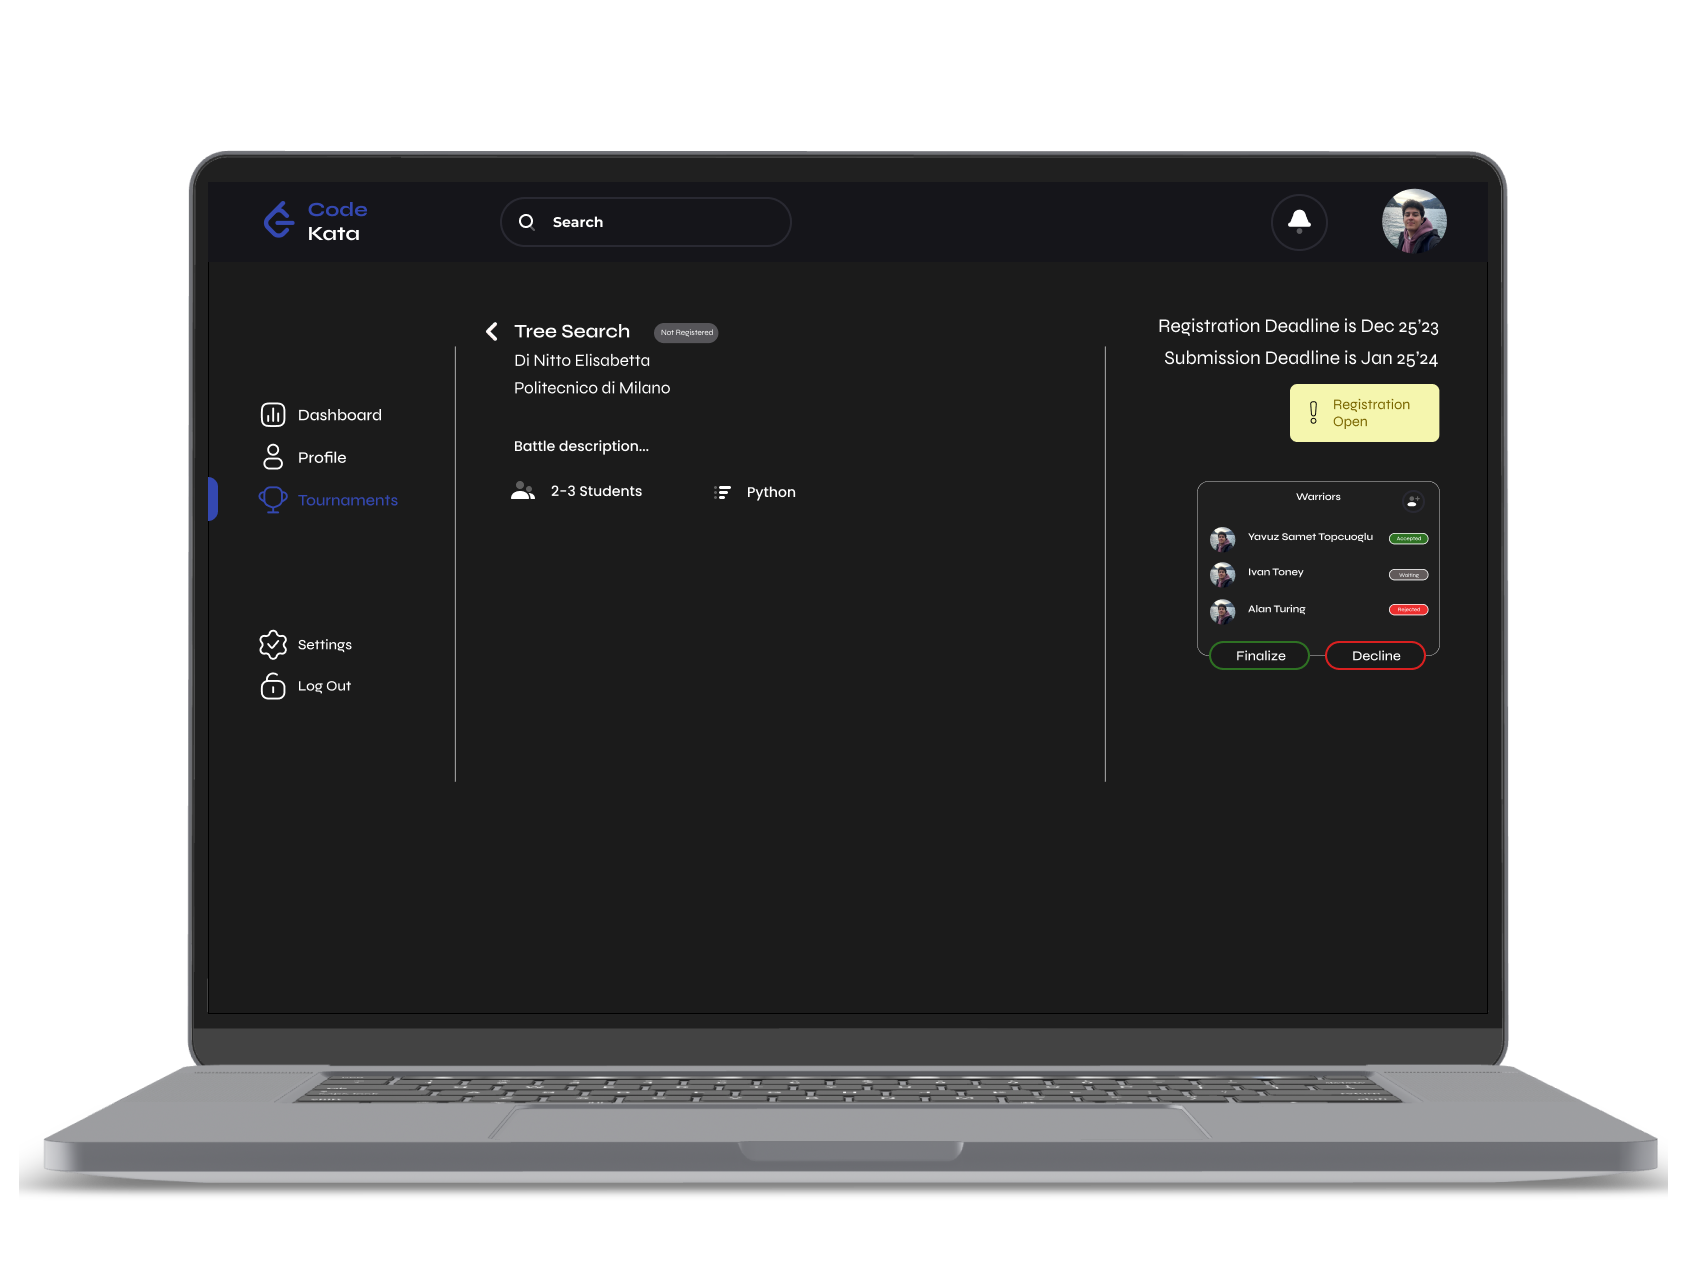
\includegraphics[scale=0.13]{Images/ui-ux/student_battle_1.png}
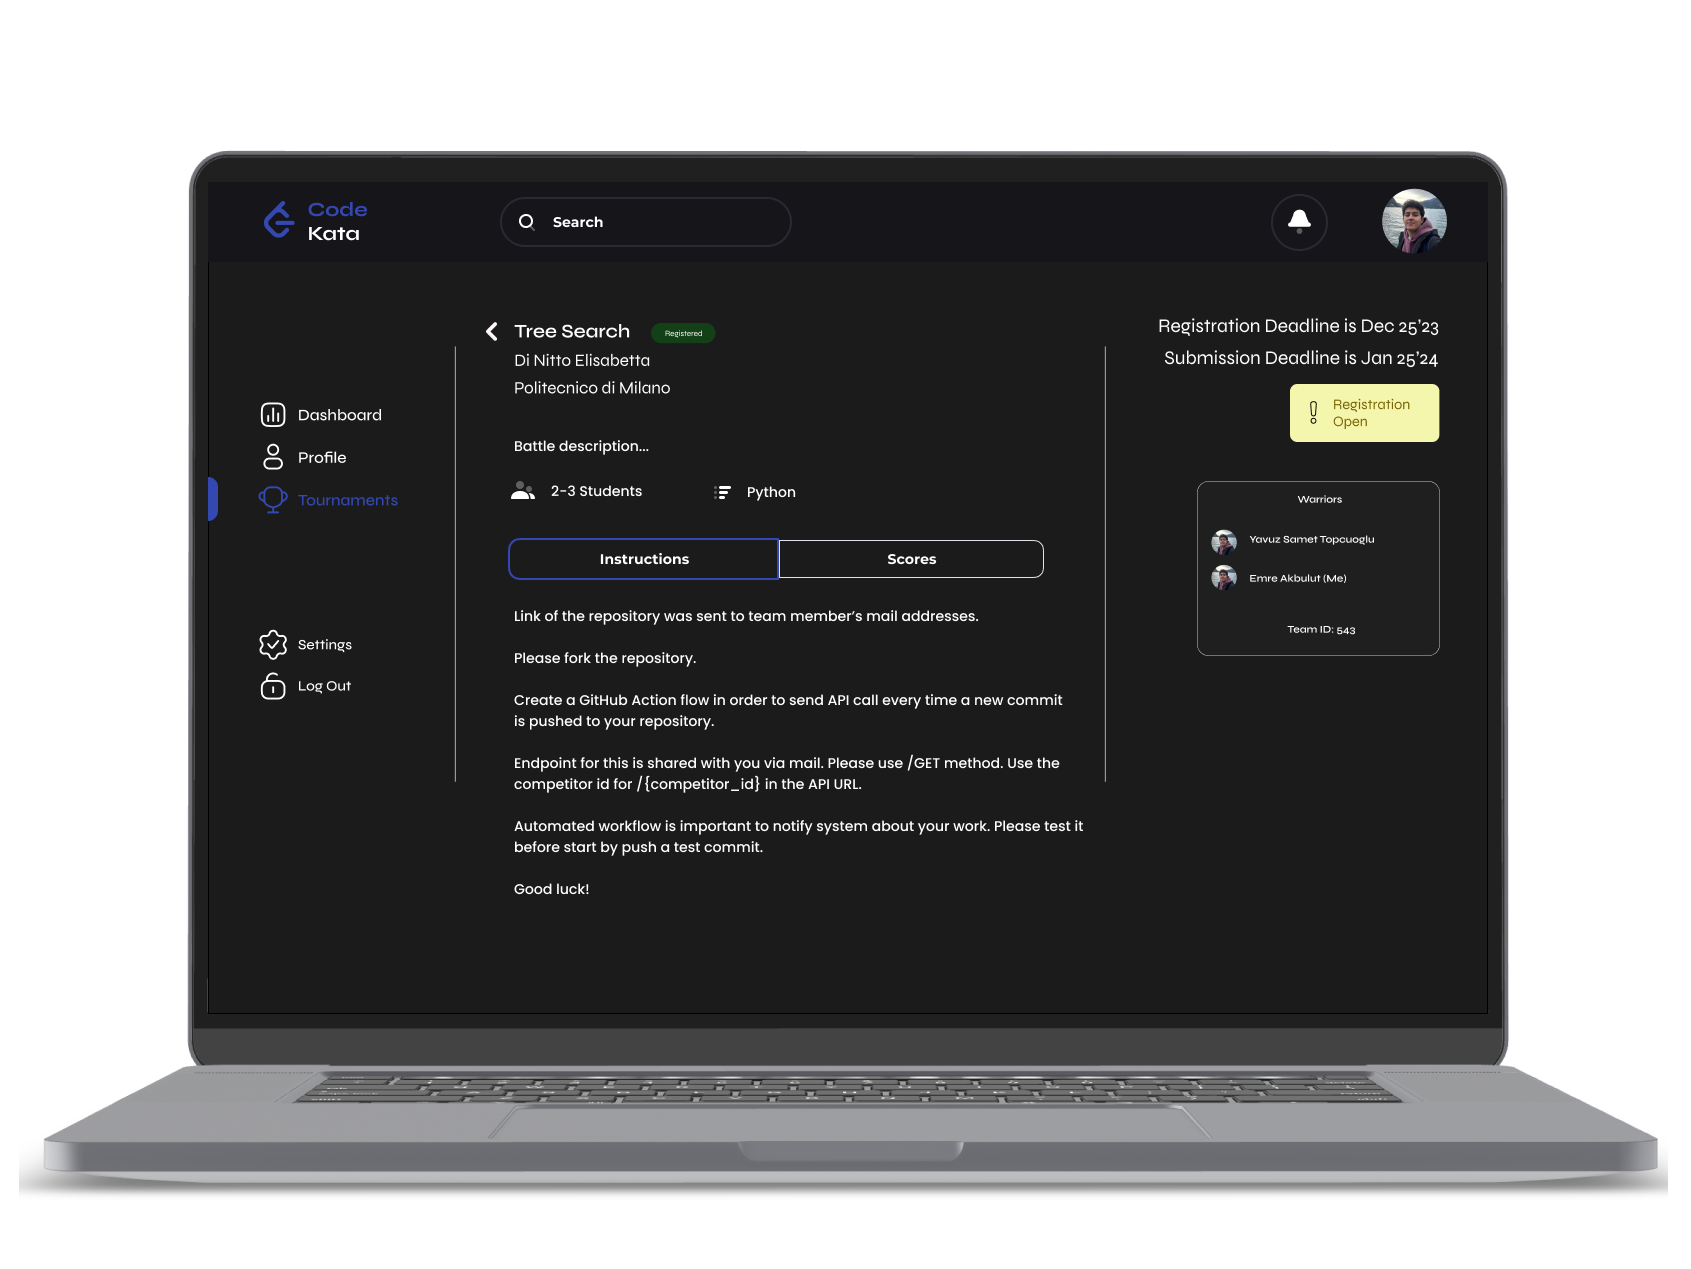
\includegraphics[scale=0.13]{Images/ui-ux/student_battle_2.png}
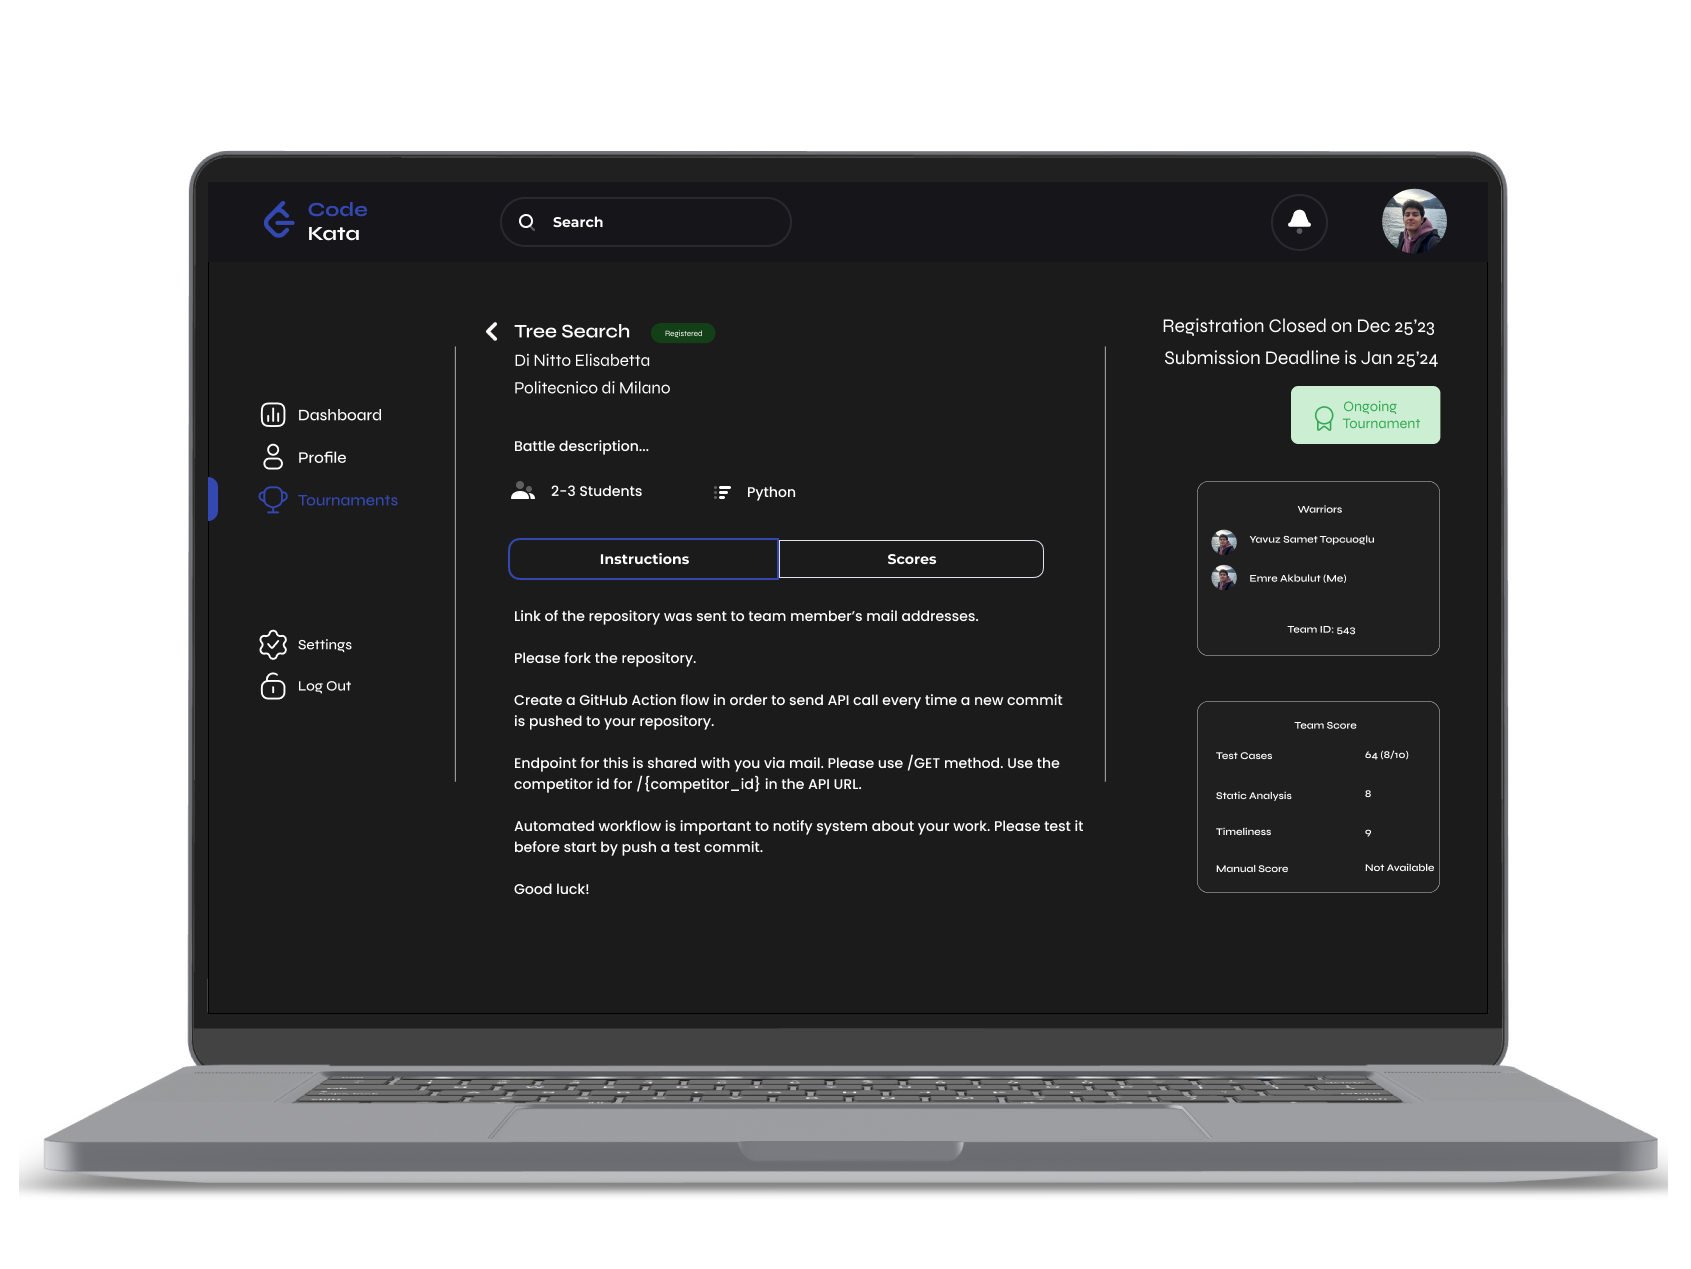
\includegraphics[scale=0.13]{Images/ui-ux/student_battle_3.png}
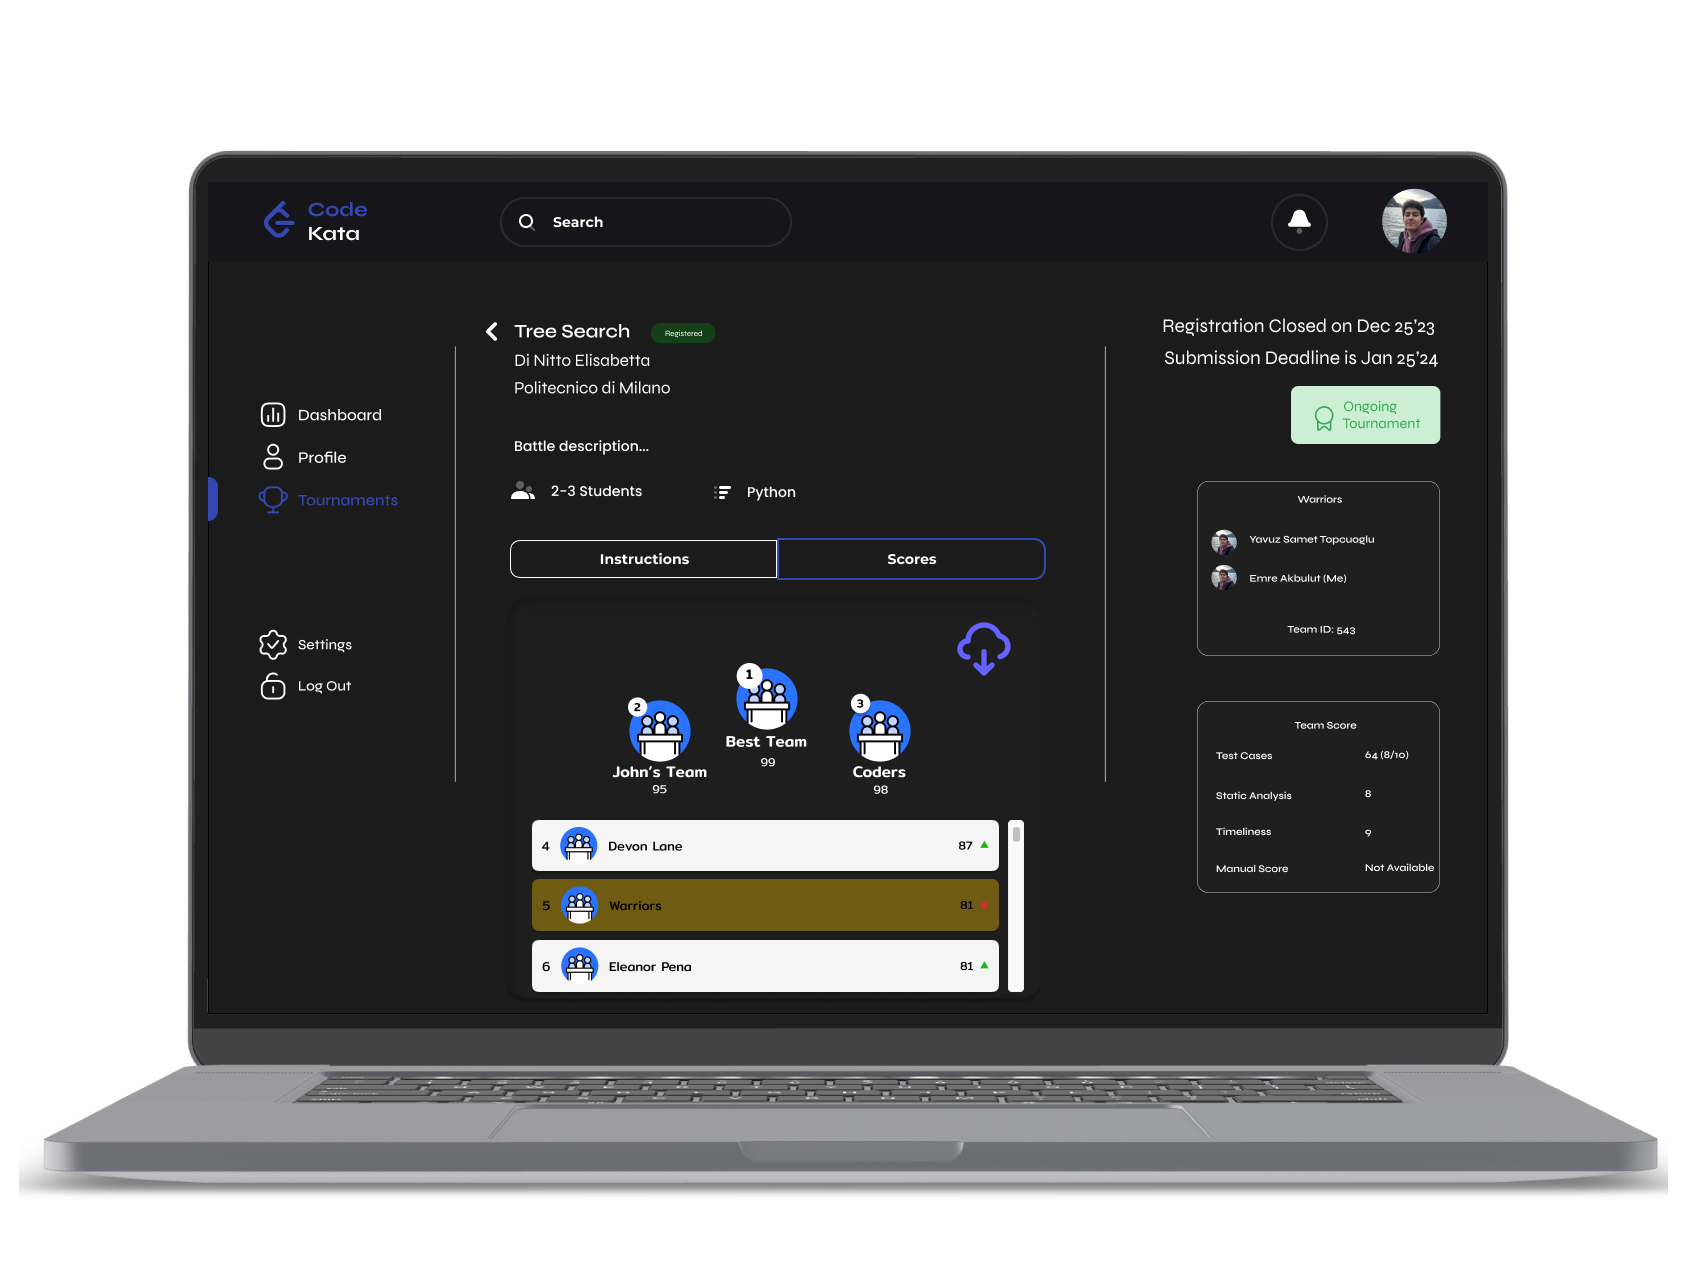
\includegraphics[scale=0.13]{Images/ui-ux/student_battle_4.png}
      (g) $UI_{7}$  Battle Screen for Student
\end{center}

\begin{center}
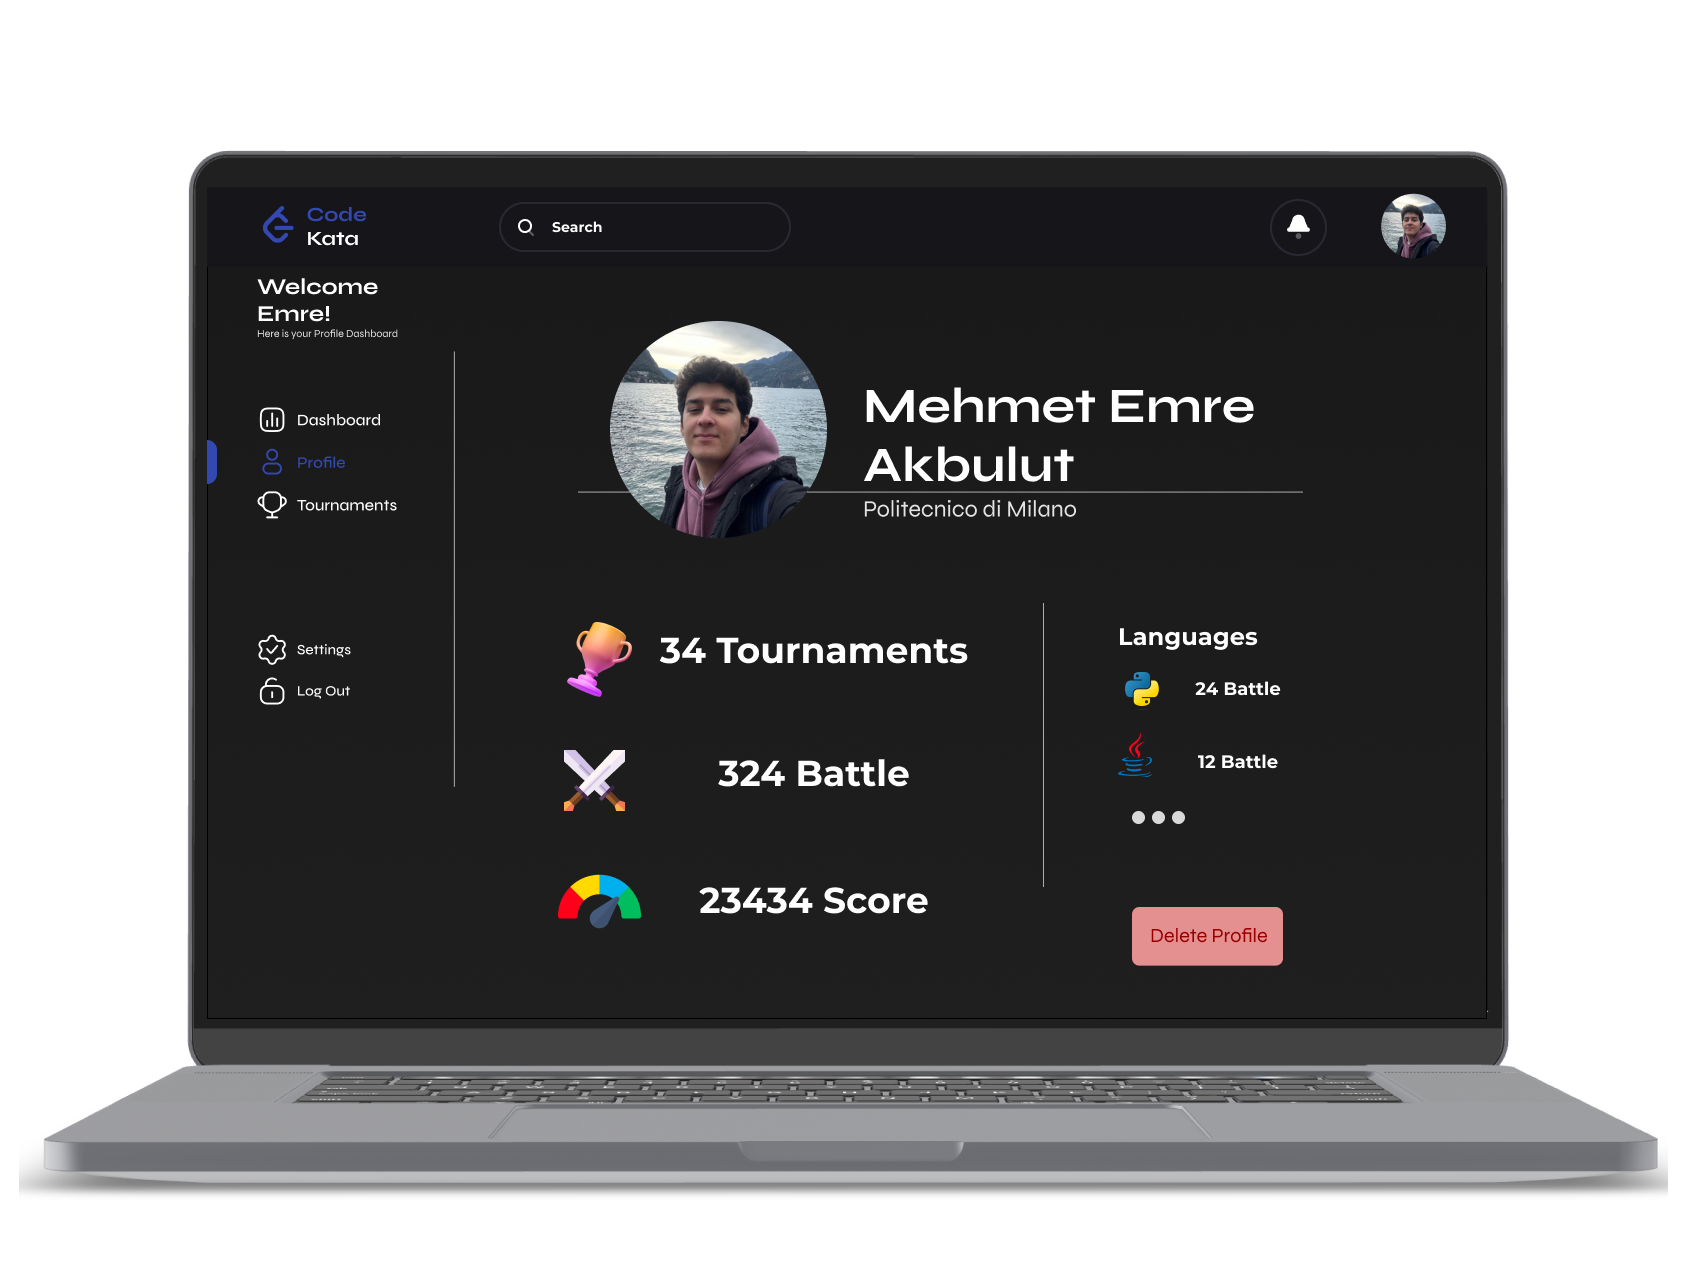
\includegraphics[scale=0.13]{Images/ui-ux/student_profile.png}
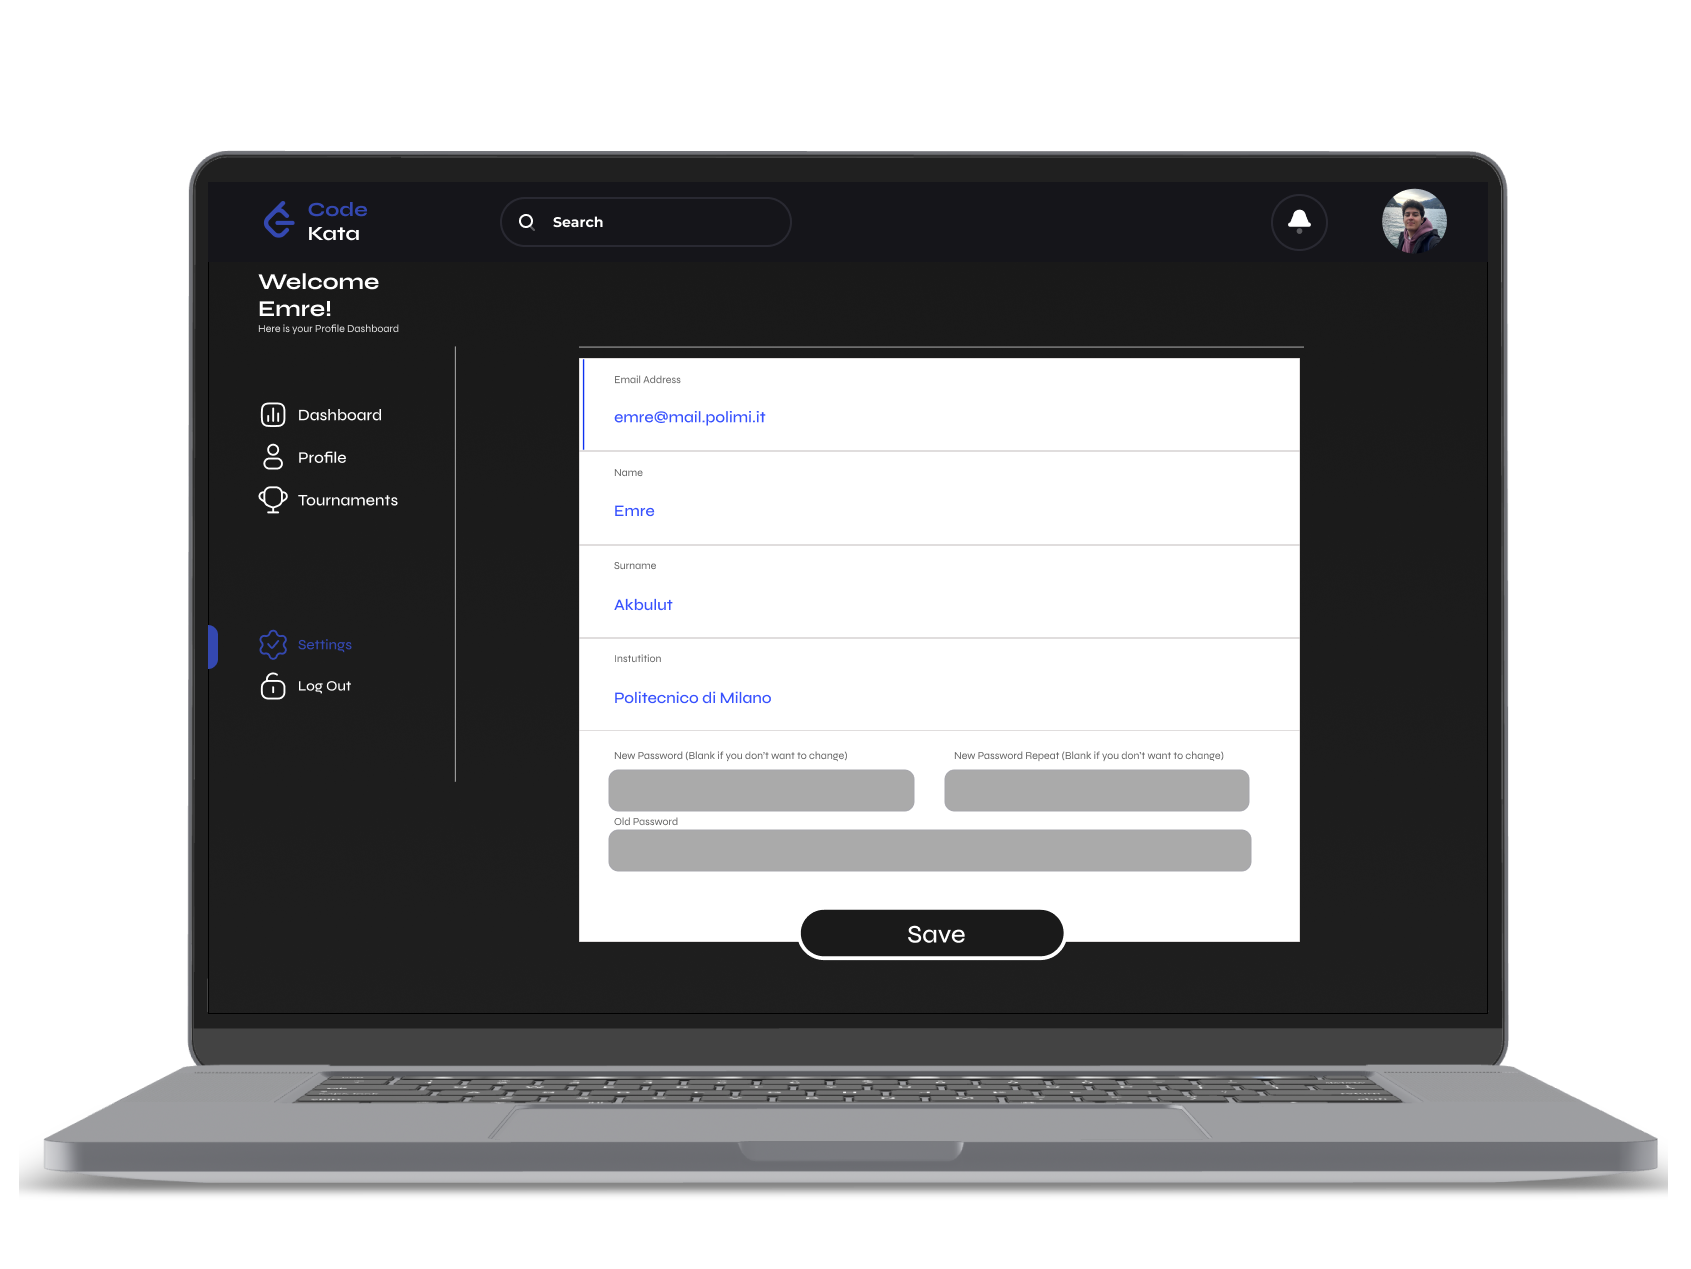
\includegraphics[scale=0.13]{Images/ui-ux/student_settings.png}
        (h) $UI_{8}$  Profile and Settings for Student
\end{center}
\newpage
\begin{center}
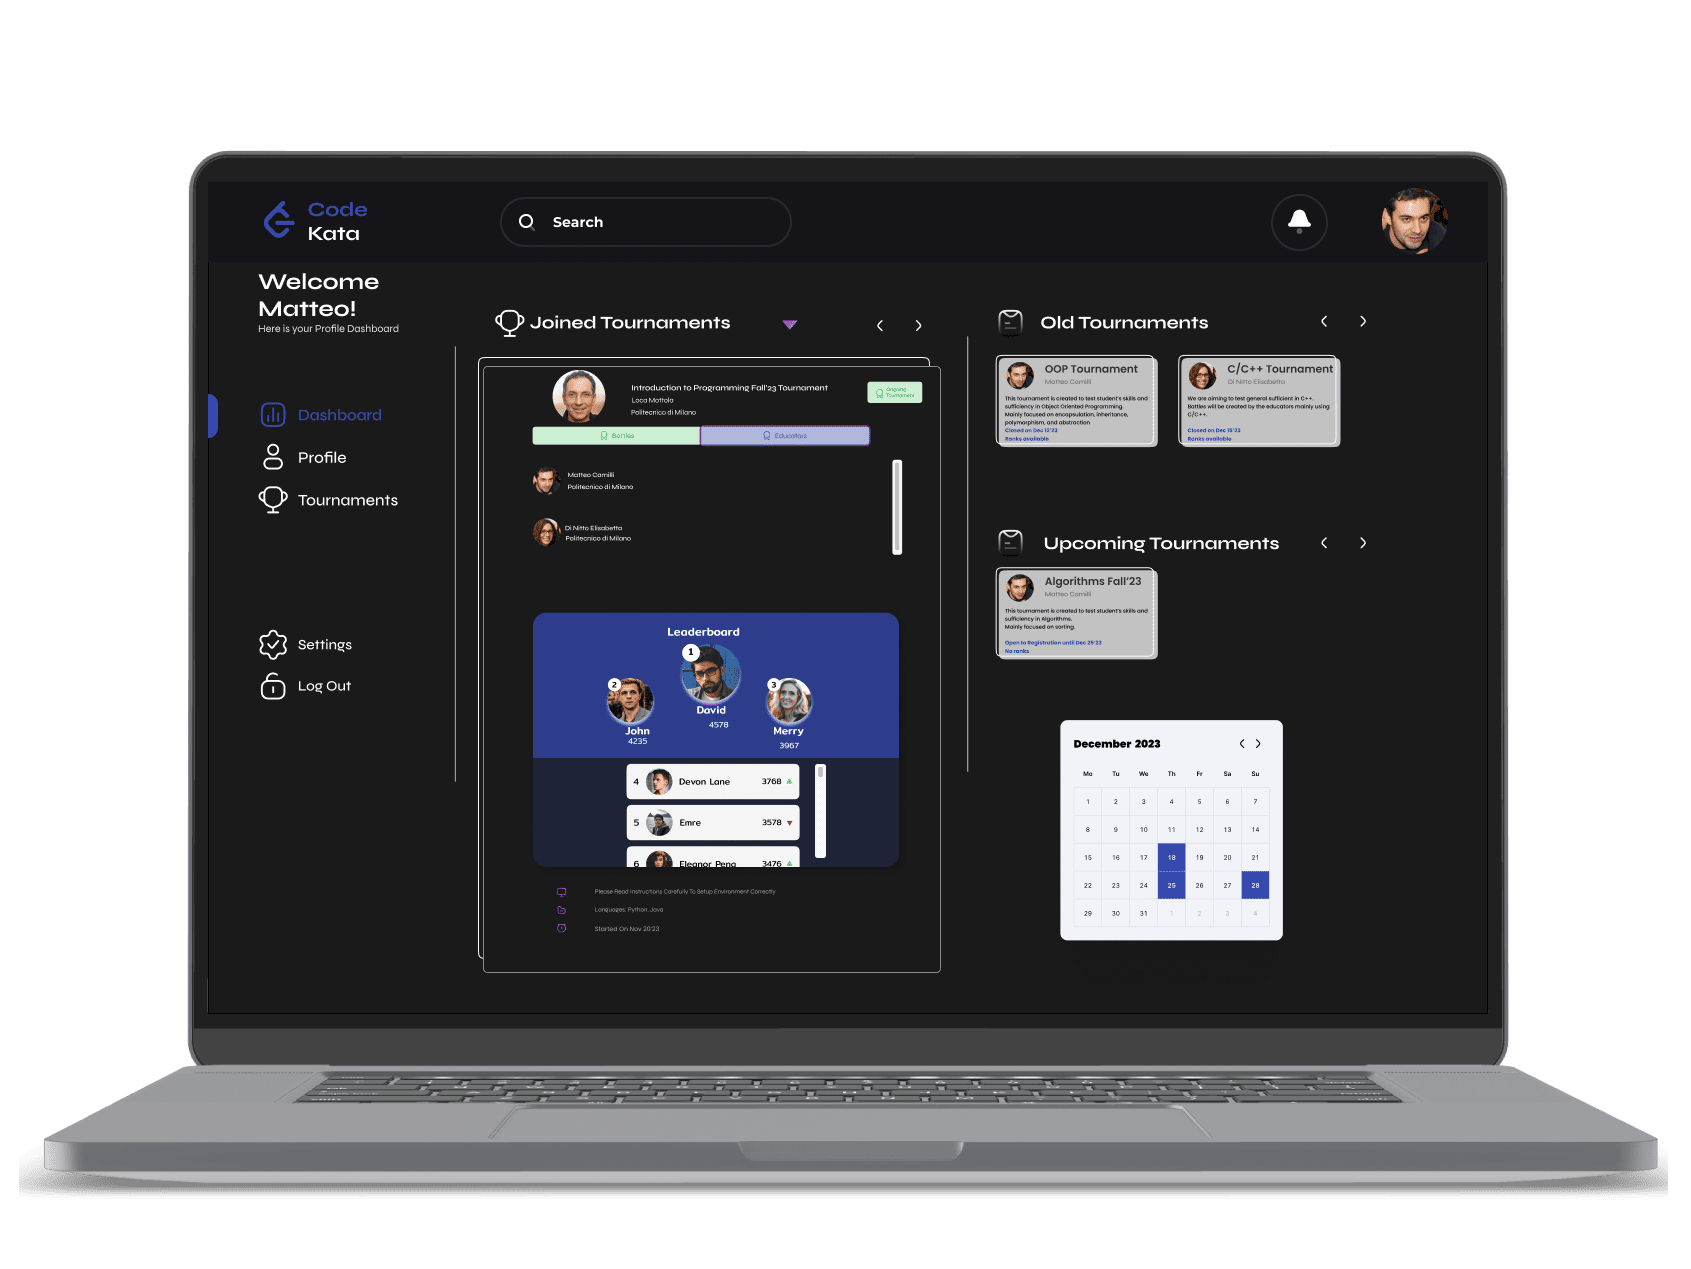
\includegraphics[scale=0.13]{Images/ui-ux/educator_dashboard_1.png}
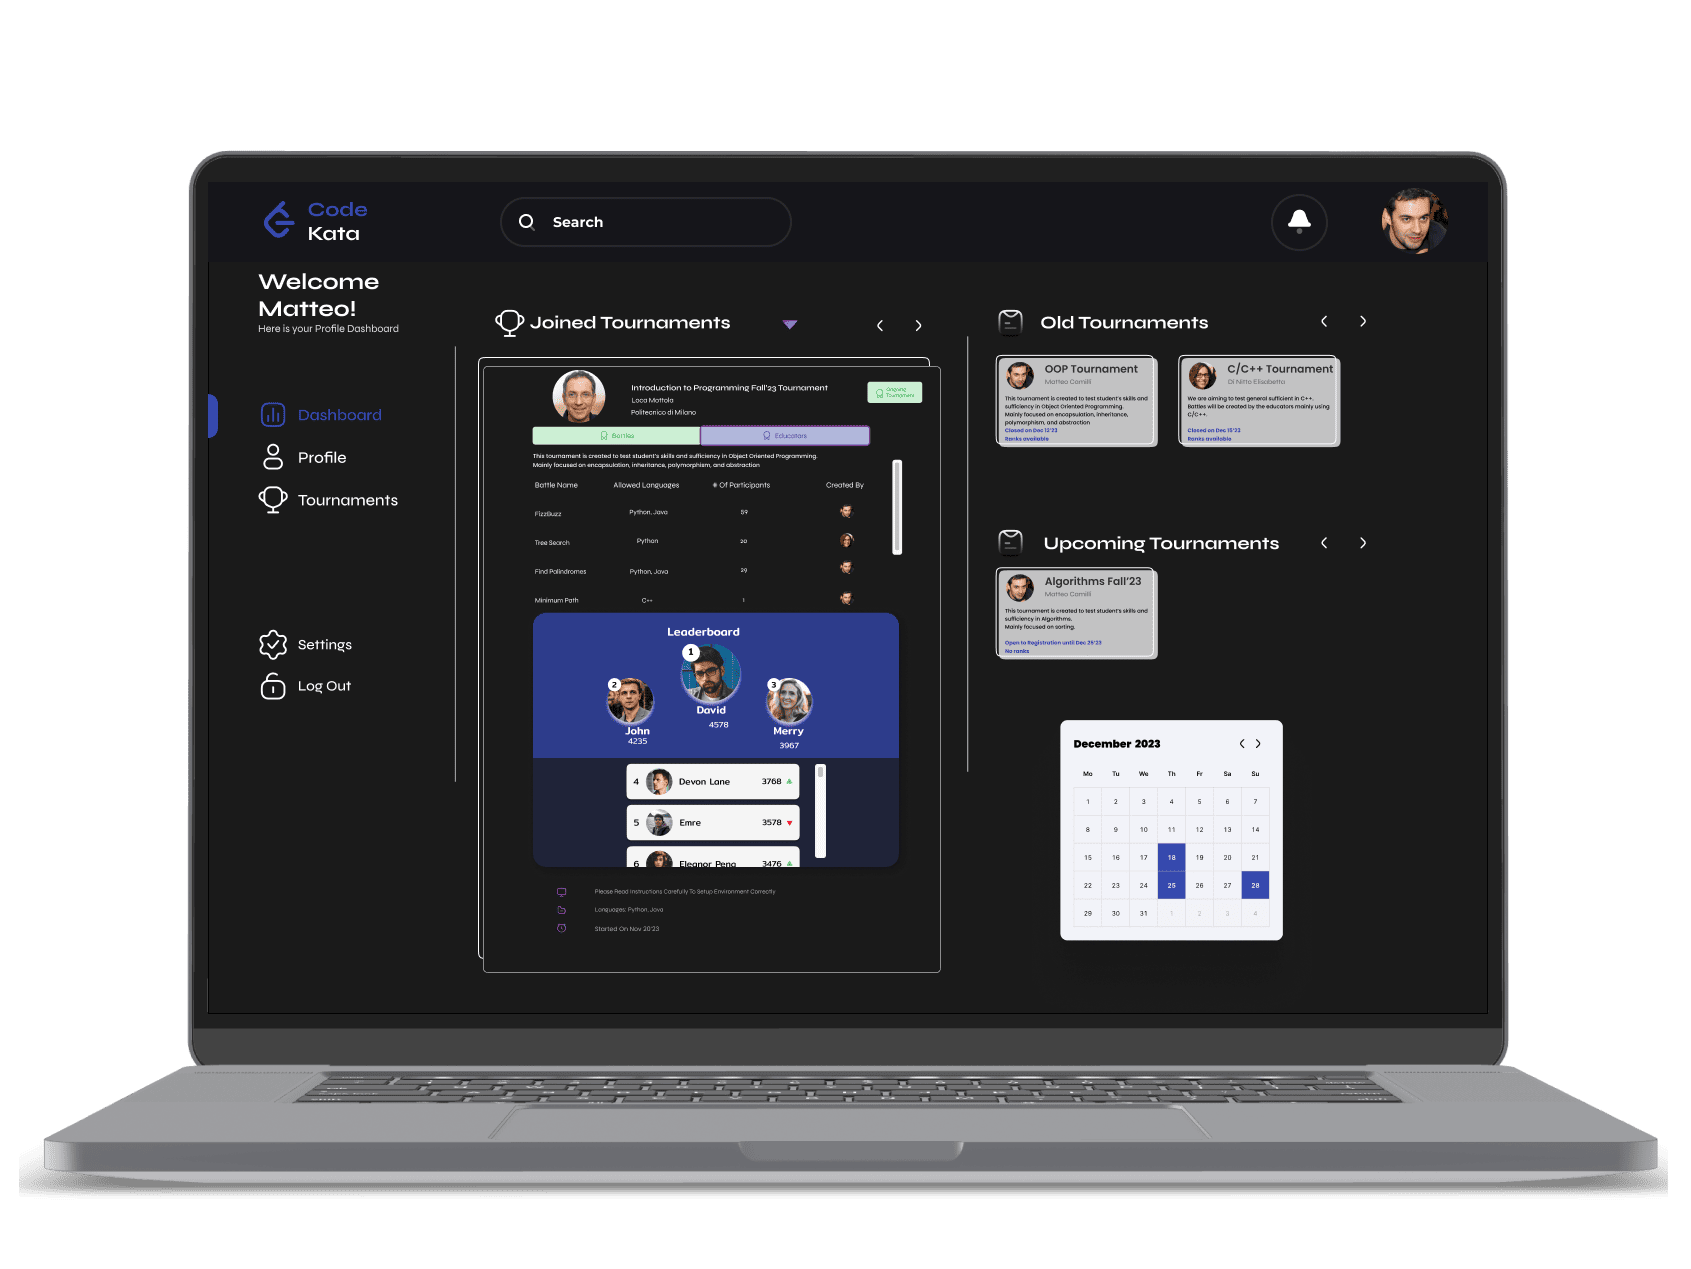
\includegraphics[scale=0.13]{Images/ui-ux/educator_dashboard_2.png}
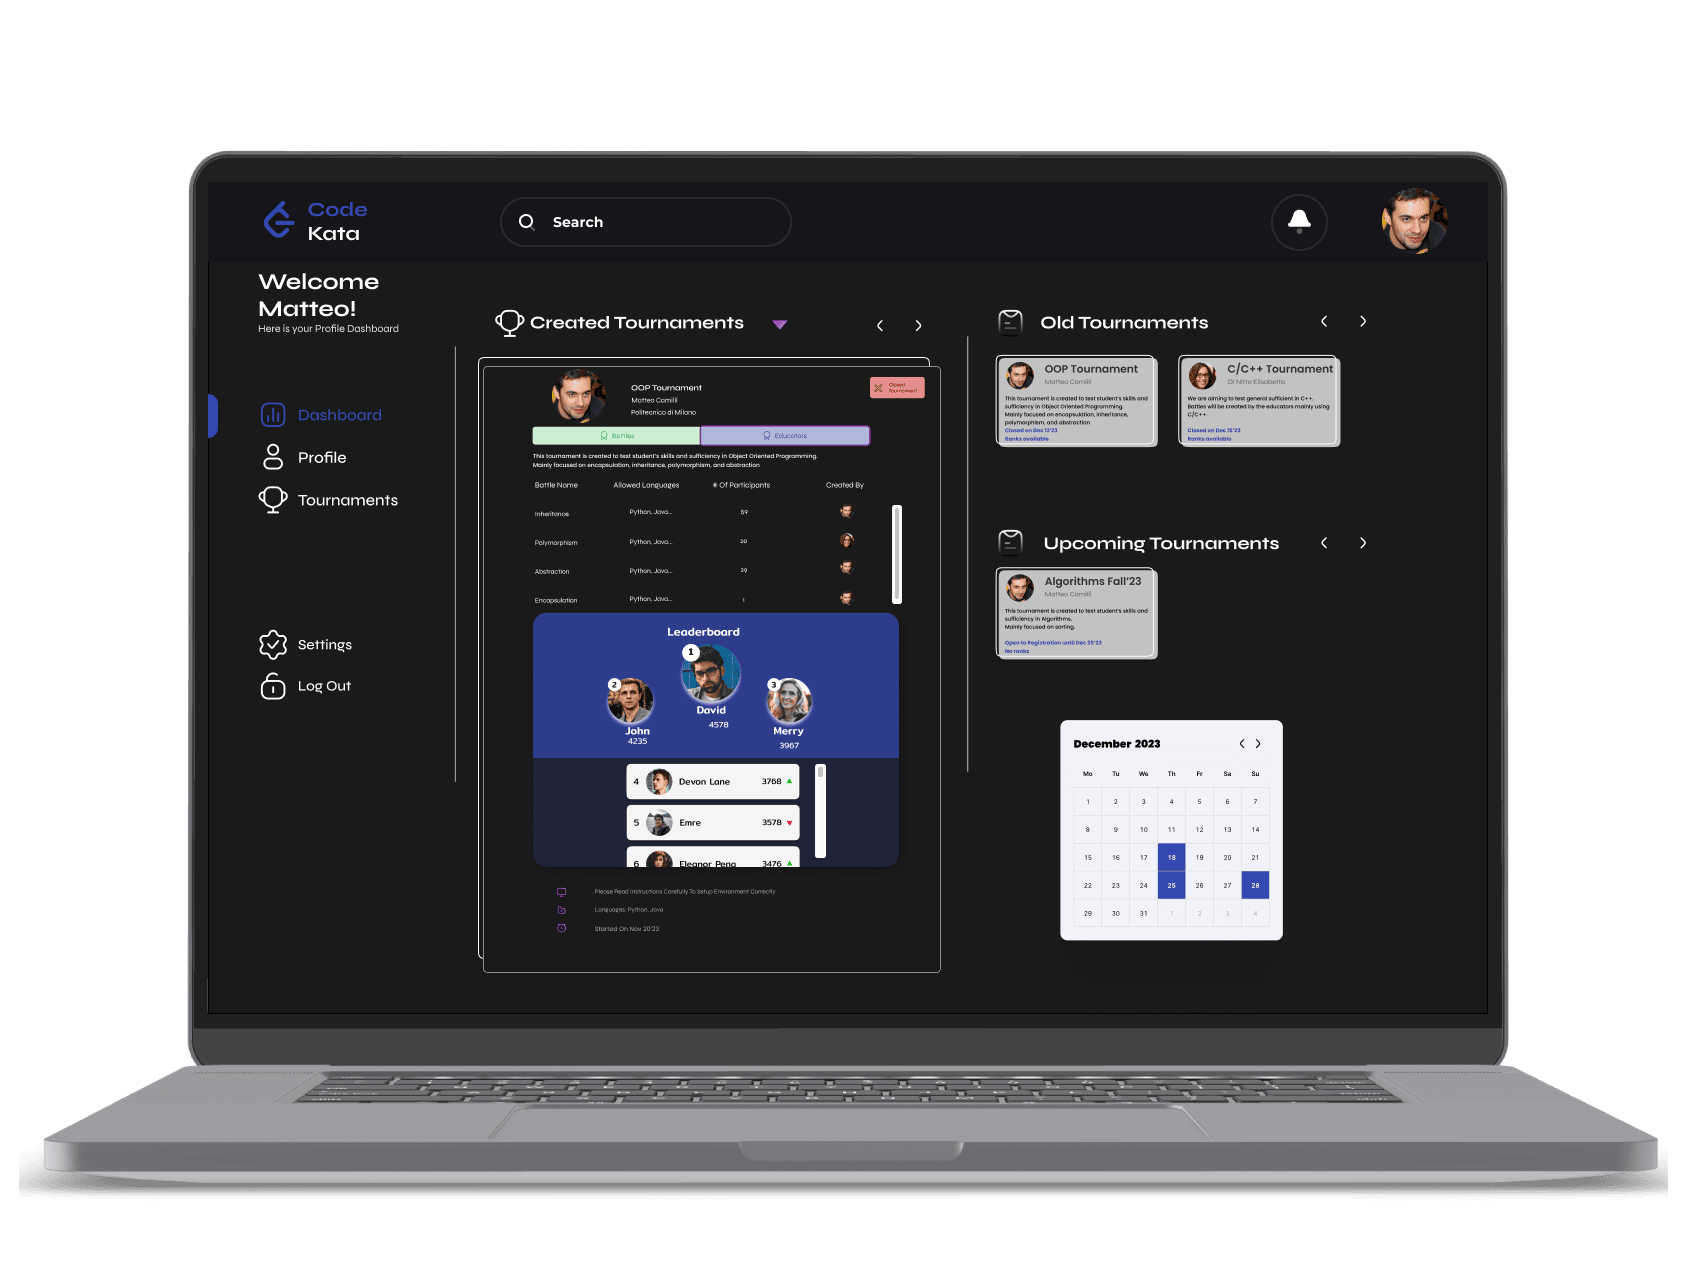
\includegraphics[scale=0.13]{Images/ui-ux/educator_dashboard_3.png}
\\ (i) $UI_{9}$  Educator Dashboard
\end{center}
\begin{center}
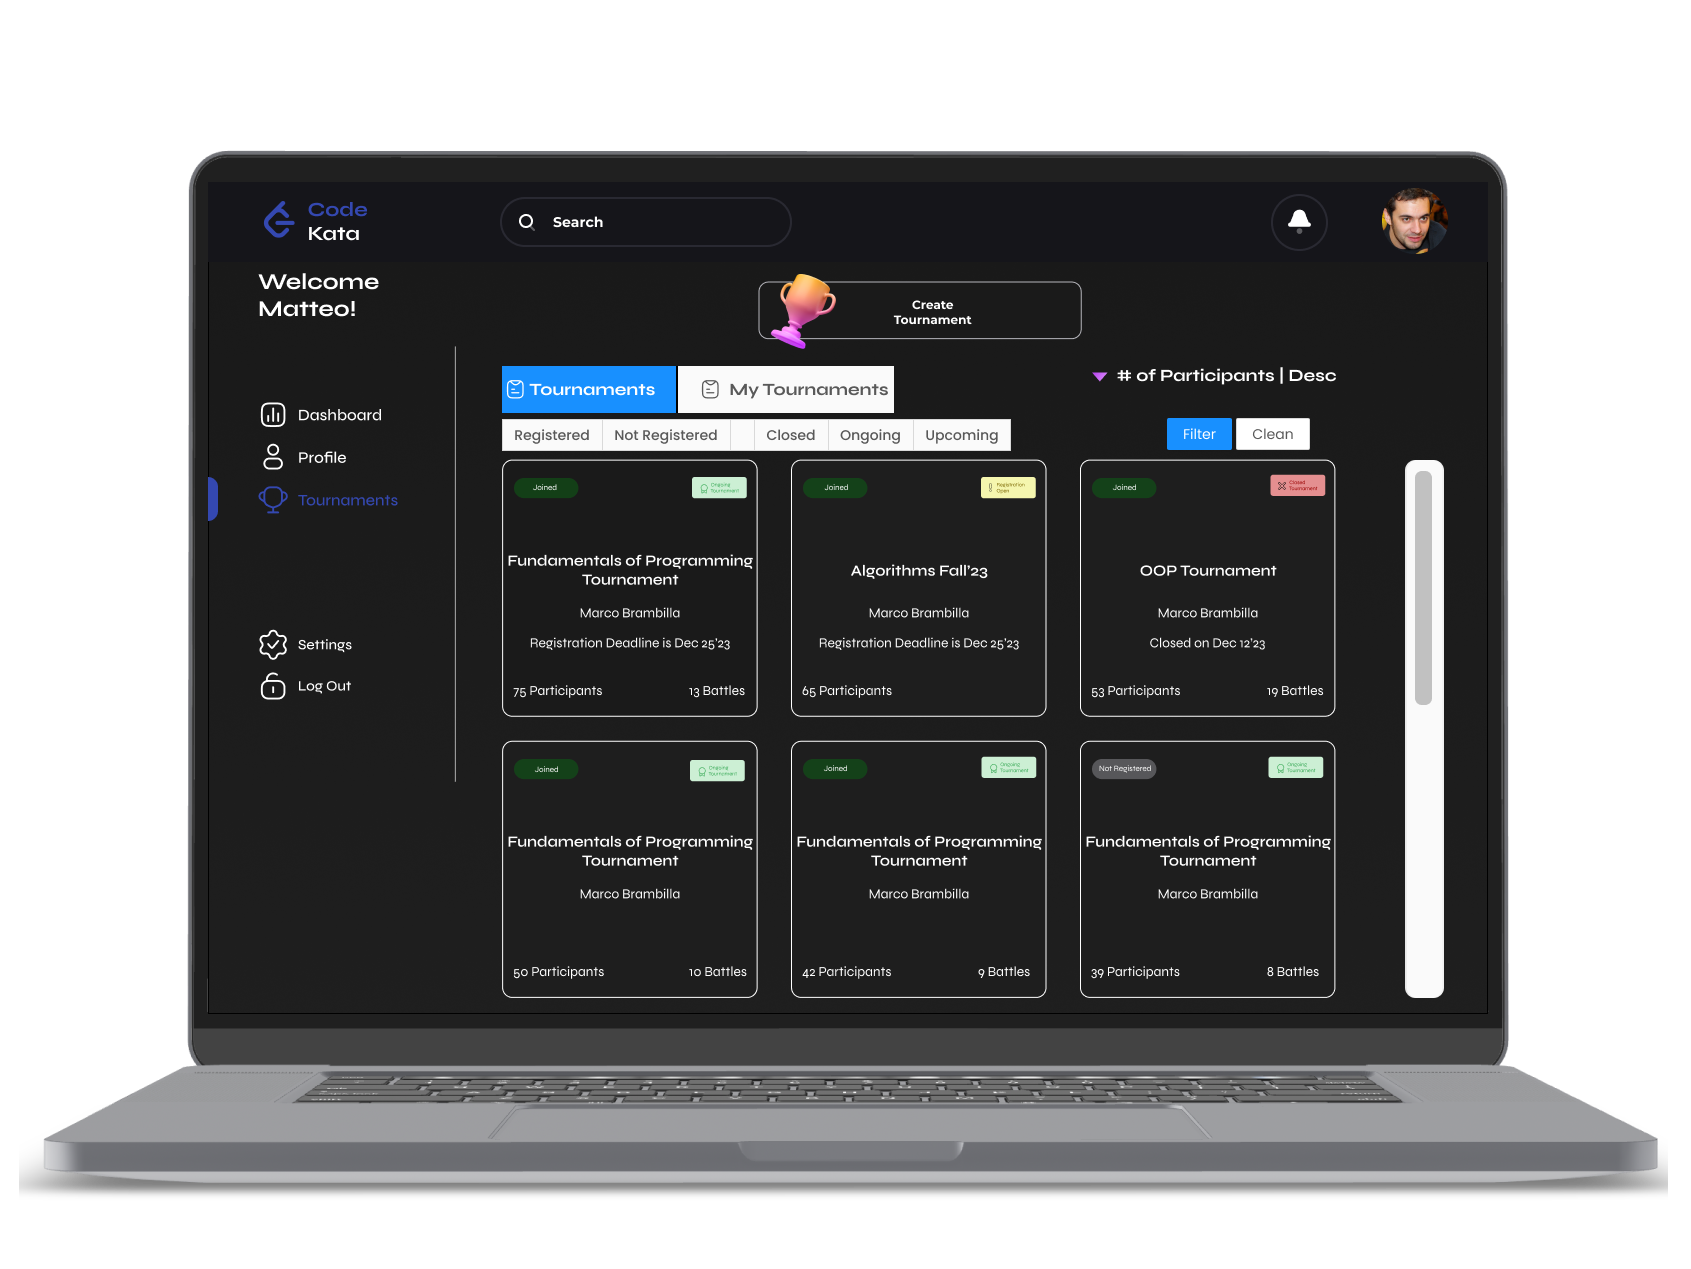
\includegraphics[scale=0.13]{Images/ui-ux/educator_tournaments_1.png}
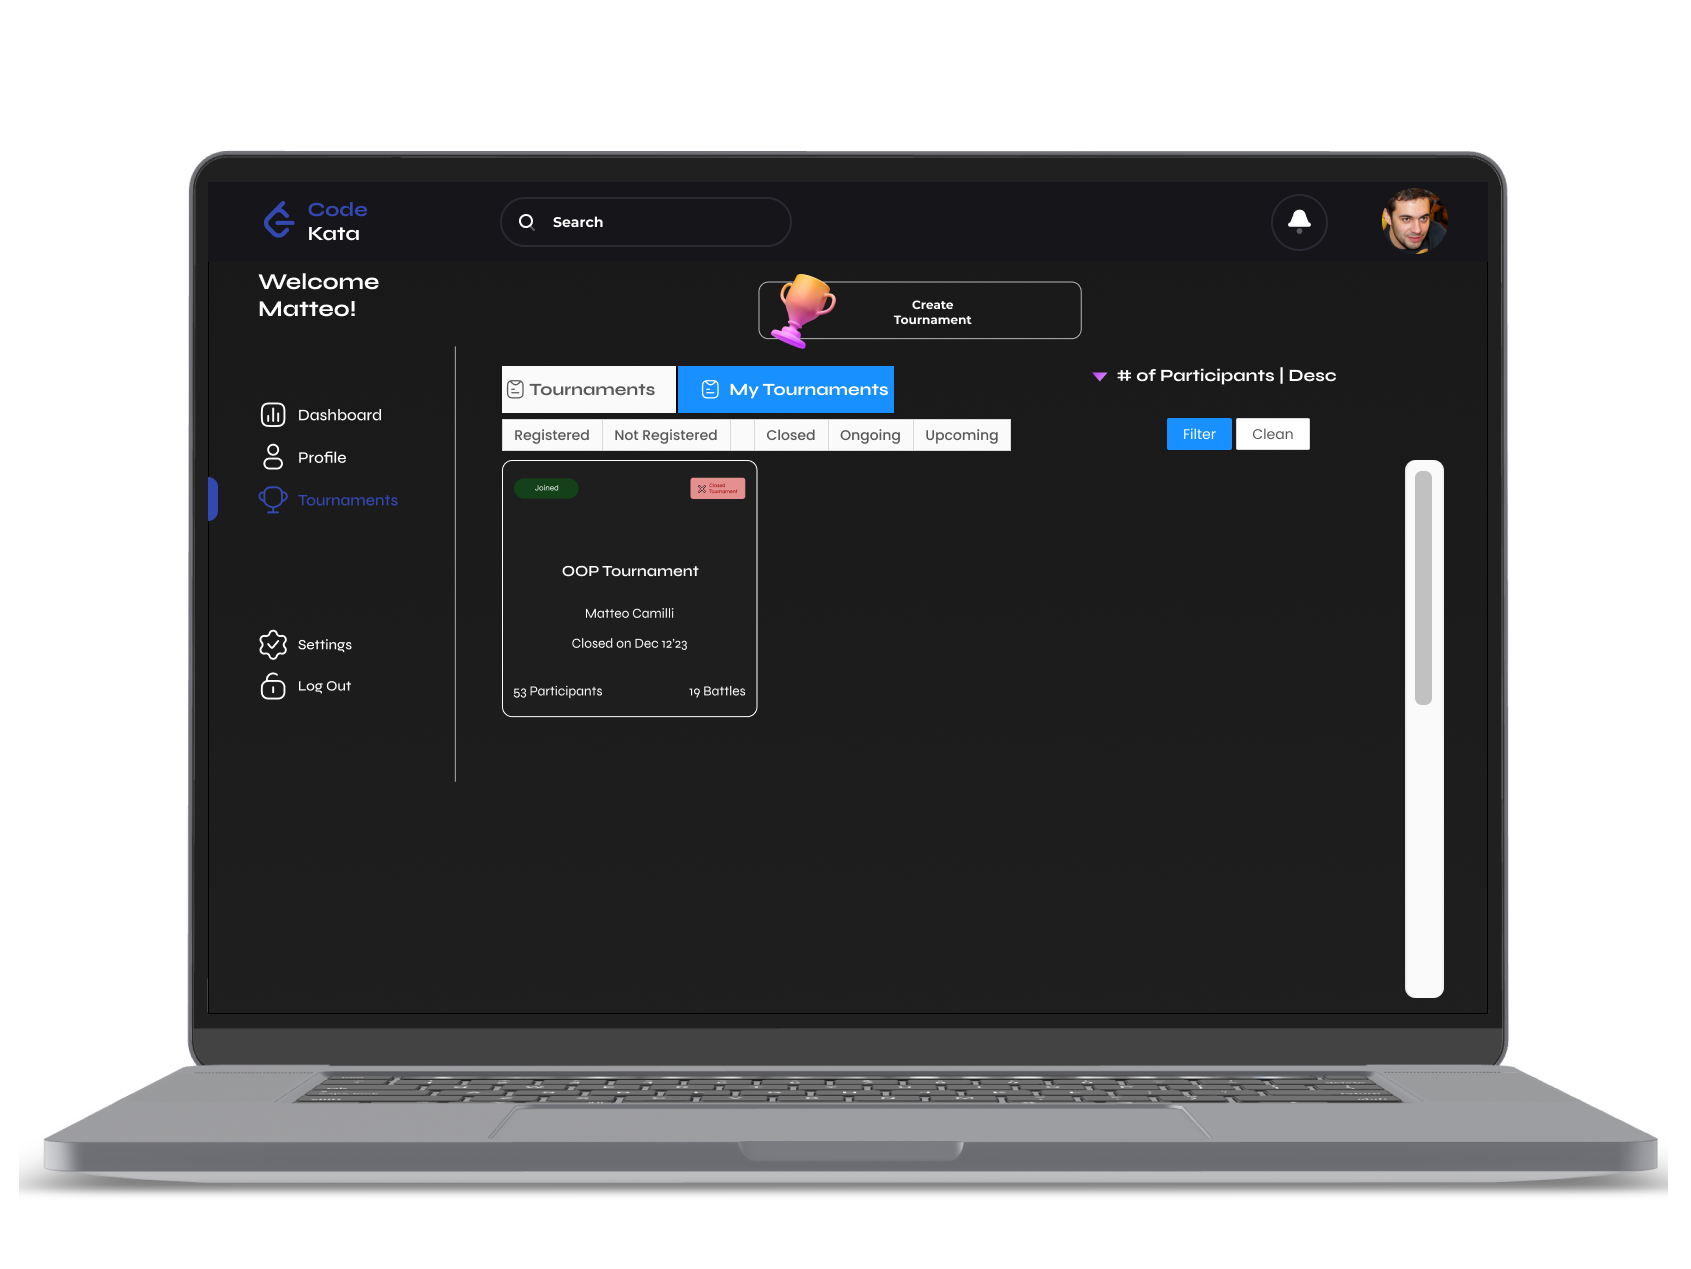
\includegraphics[scale=0.13]{Images/ui-ux/educator_tournaments_2.png}
        (j) $UI_{10}$  Educator Tournaments
\end{center}
\begin{center}
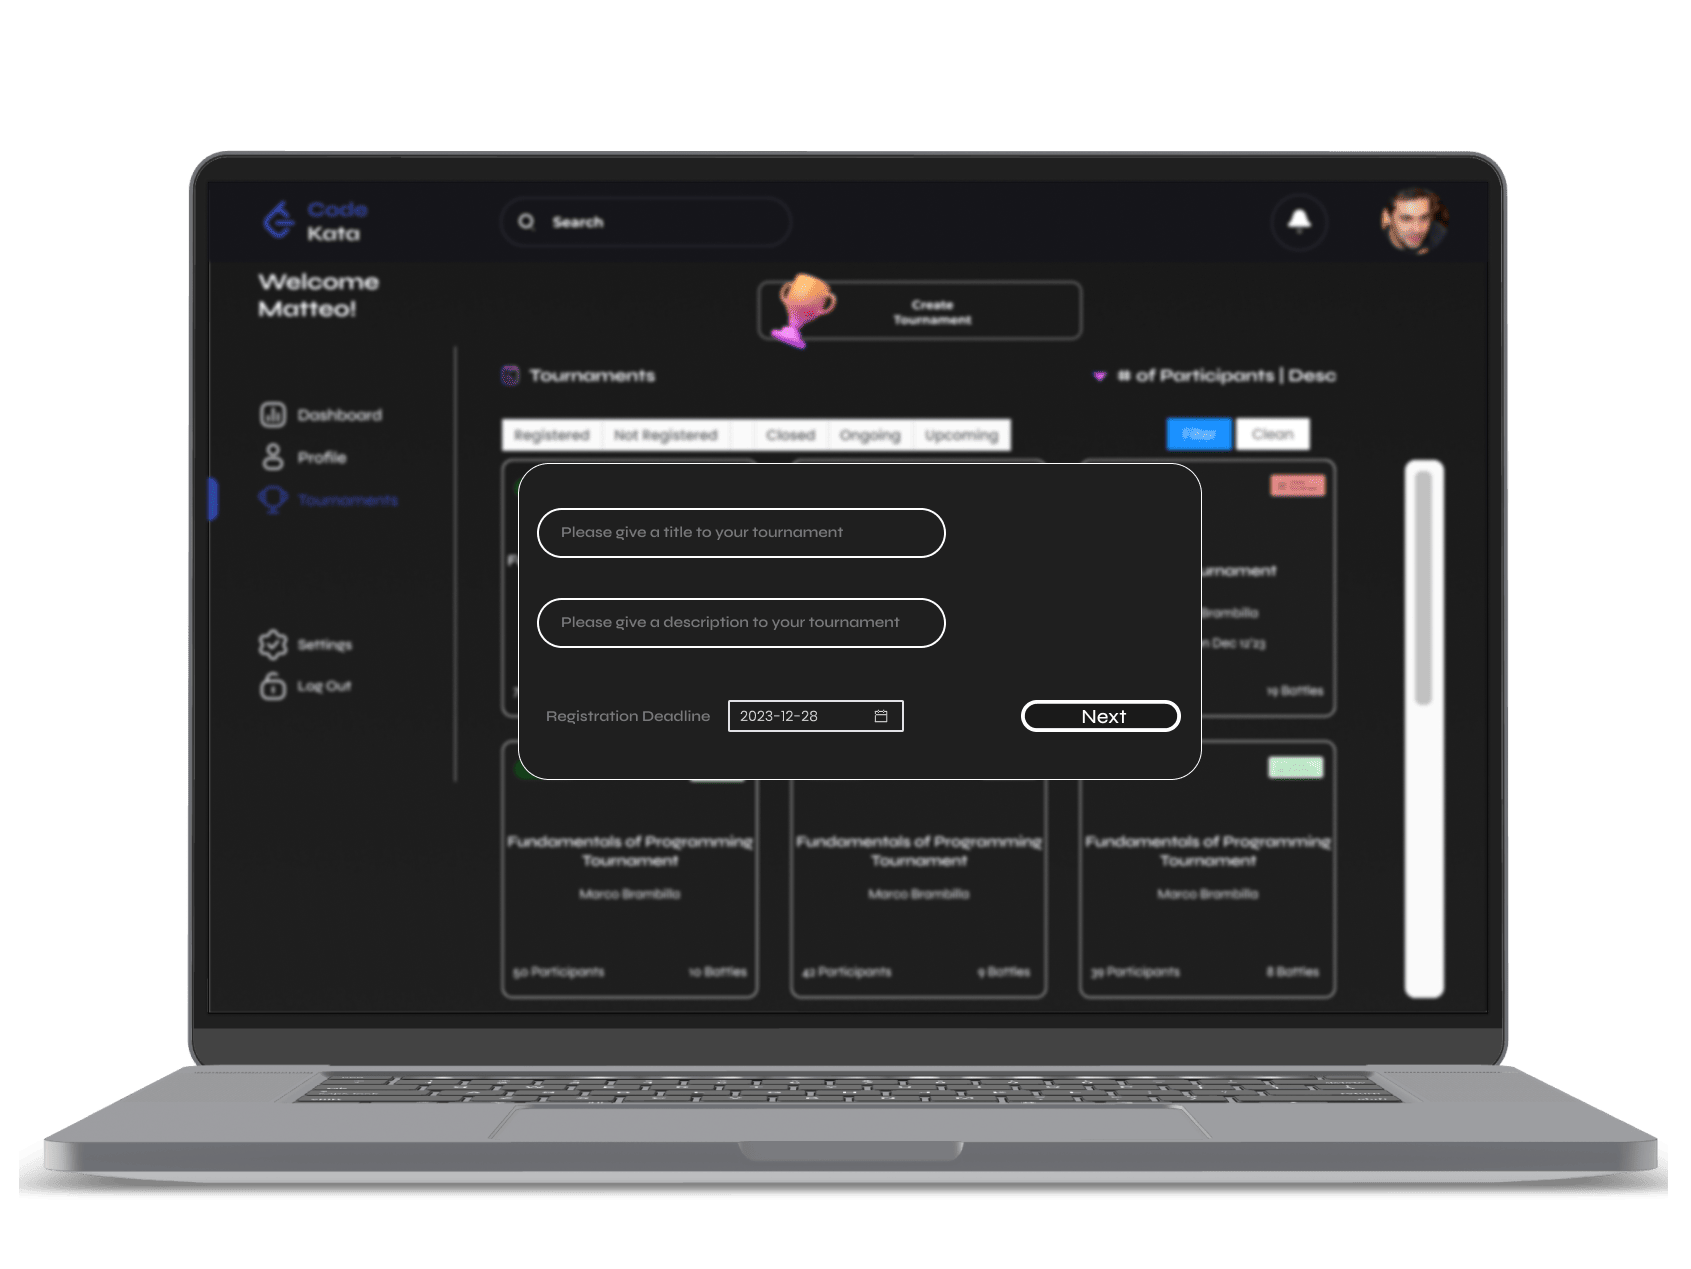
\includegraphics[scale=0.13]{Images/ui-ux/educator_create_tournament_1.png}
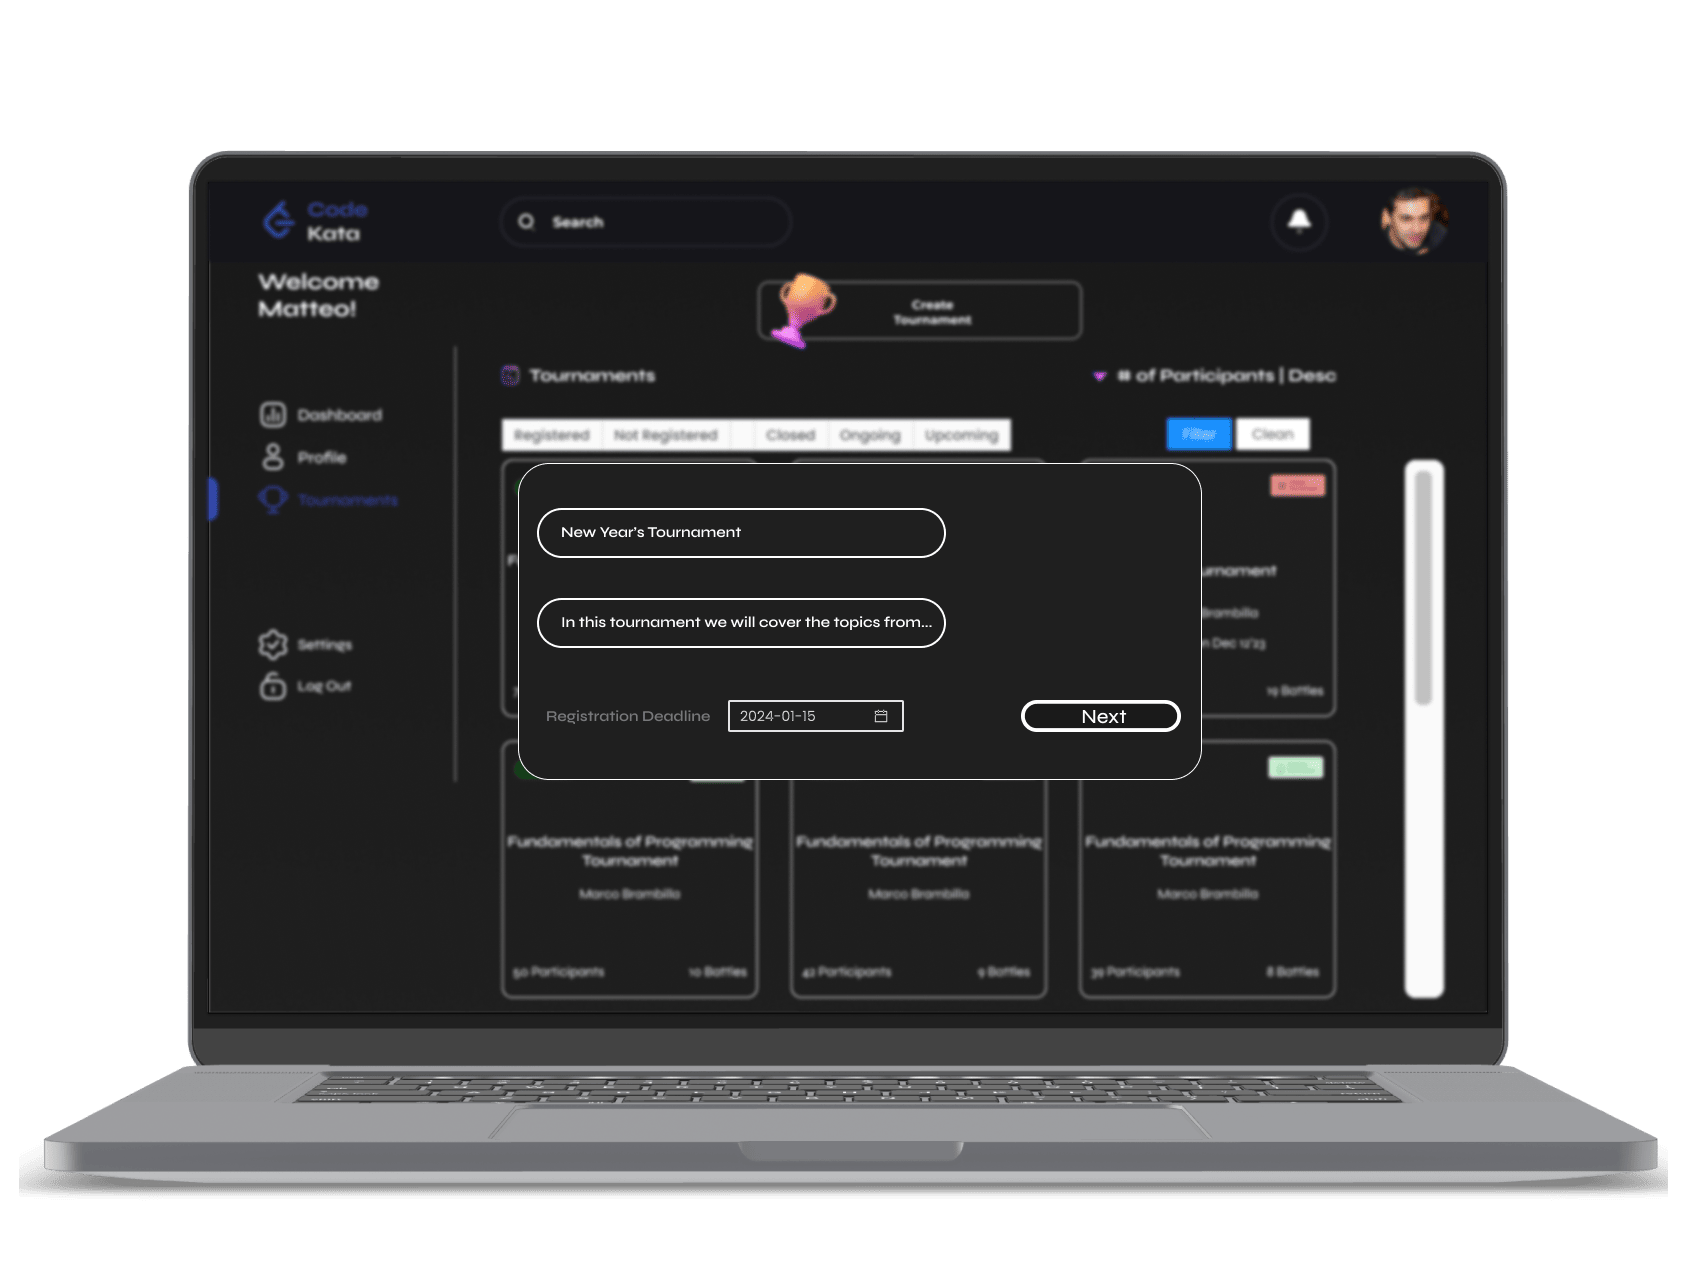
\includegraphics[scale=0.13]{Images/ui-ux/educator_create_tournament_2.png}
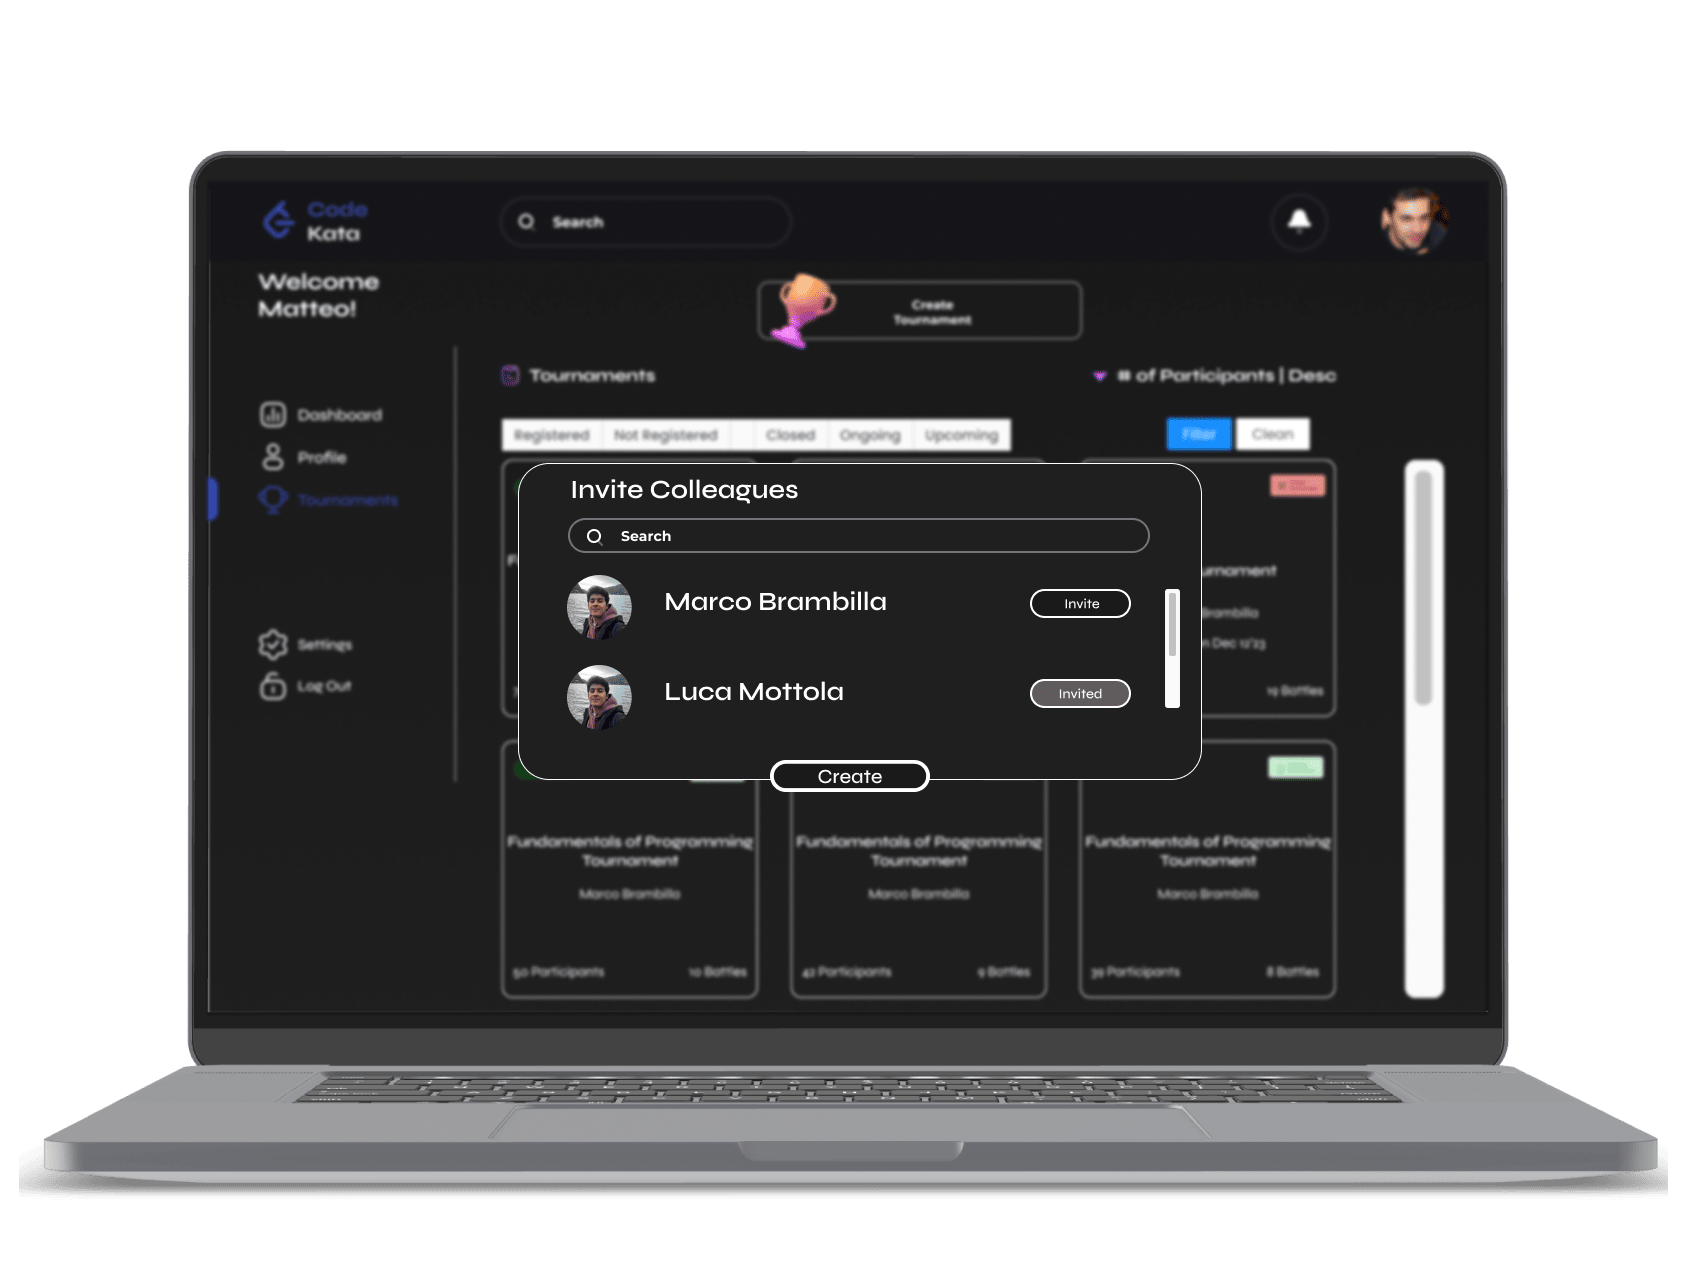
\includegraphics[scale=0.13]{Images/ui-ux/educator_create_tournament_3.png}
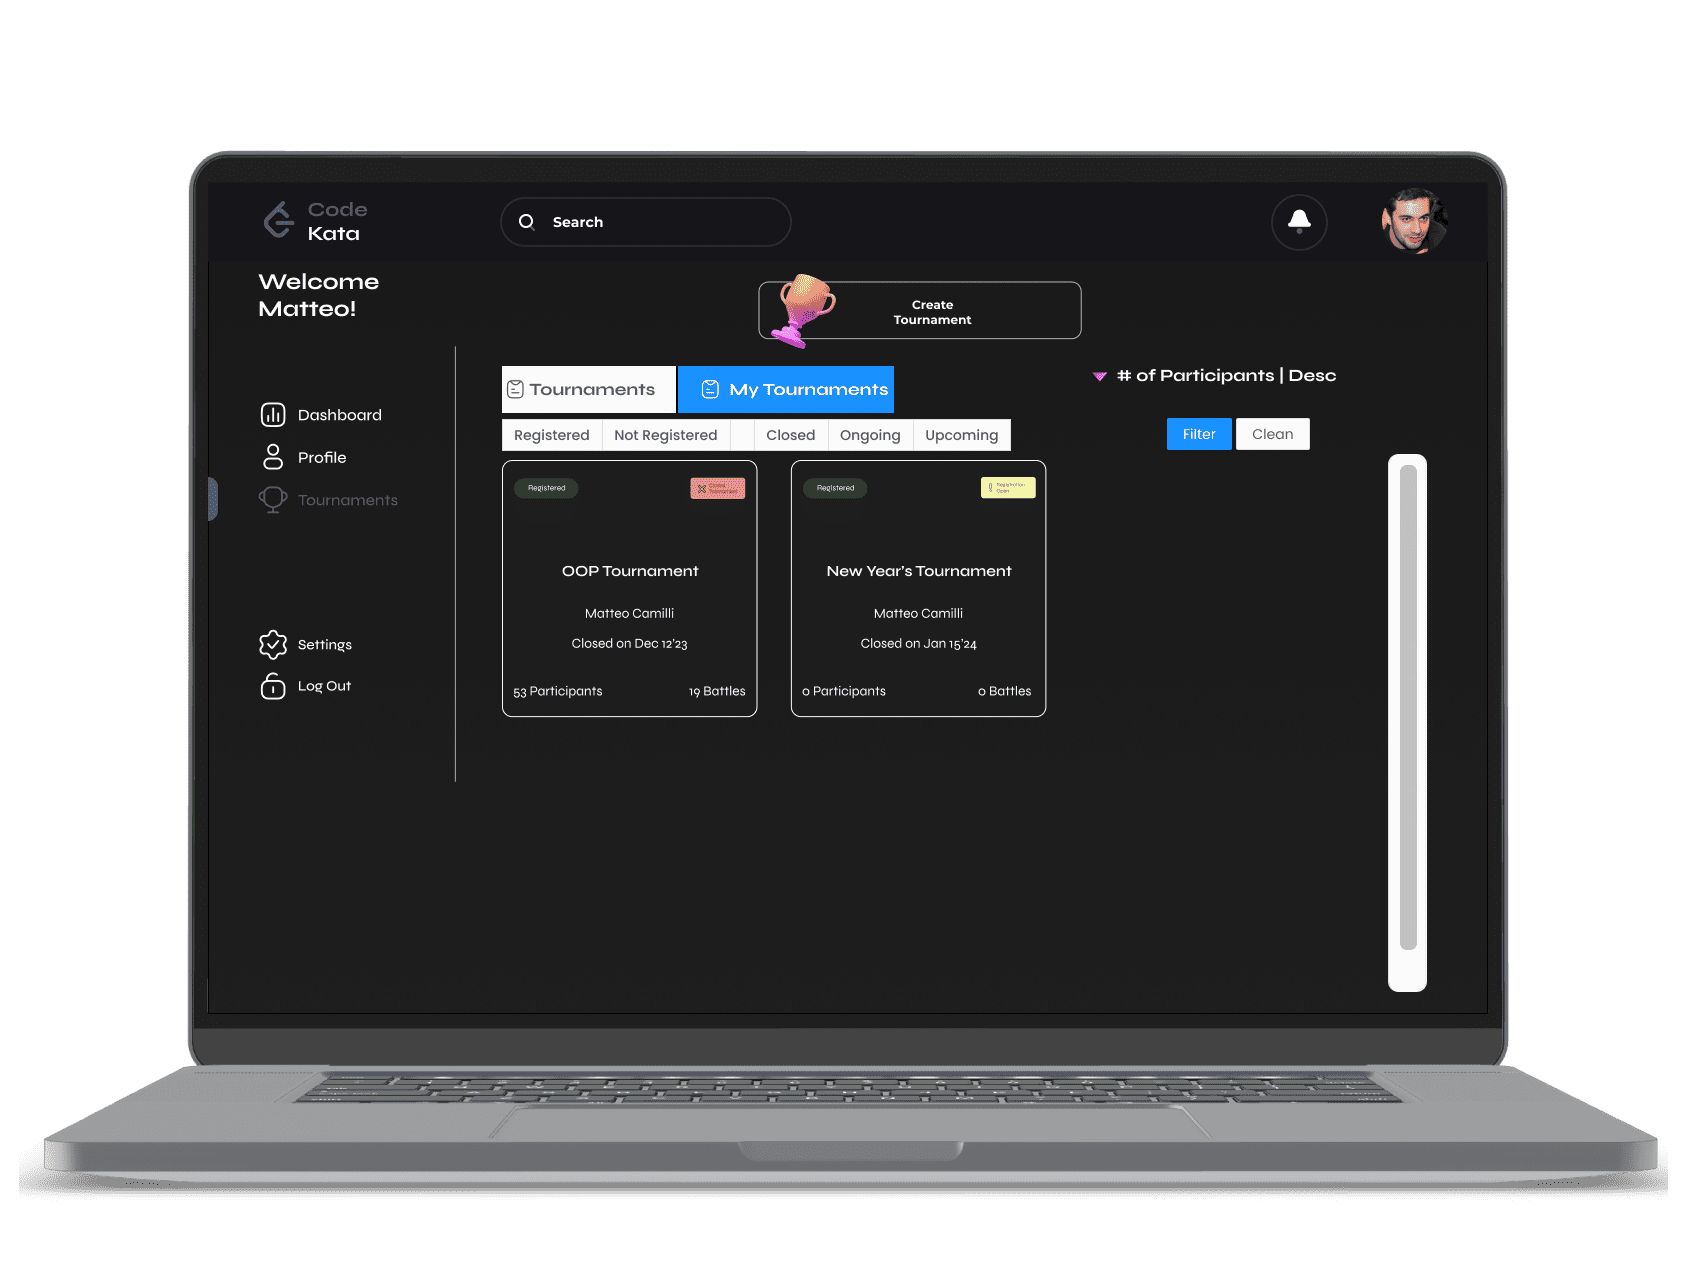
\includegraphics[scale=0.13]{Images/ui-ux/educator_create_tournament_4.png}
        (k) $UI_{11}$ Educator Creates Tournament
\end{center}
\newpage
\begin{center}
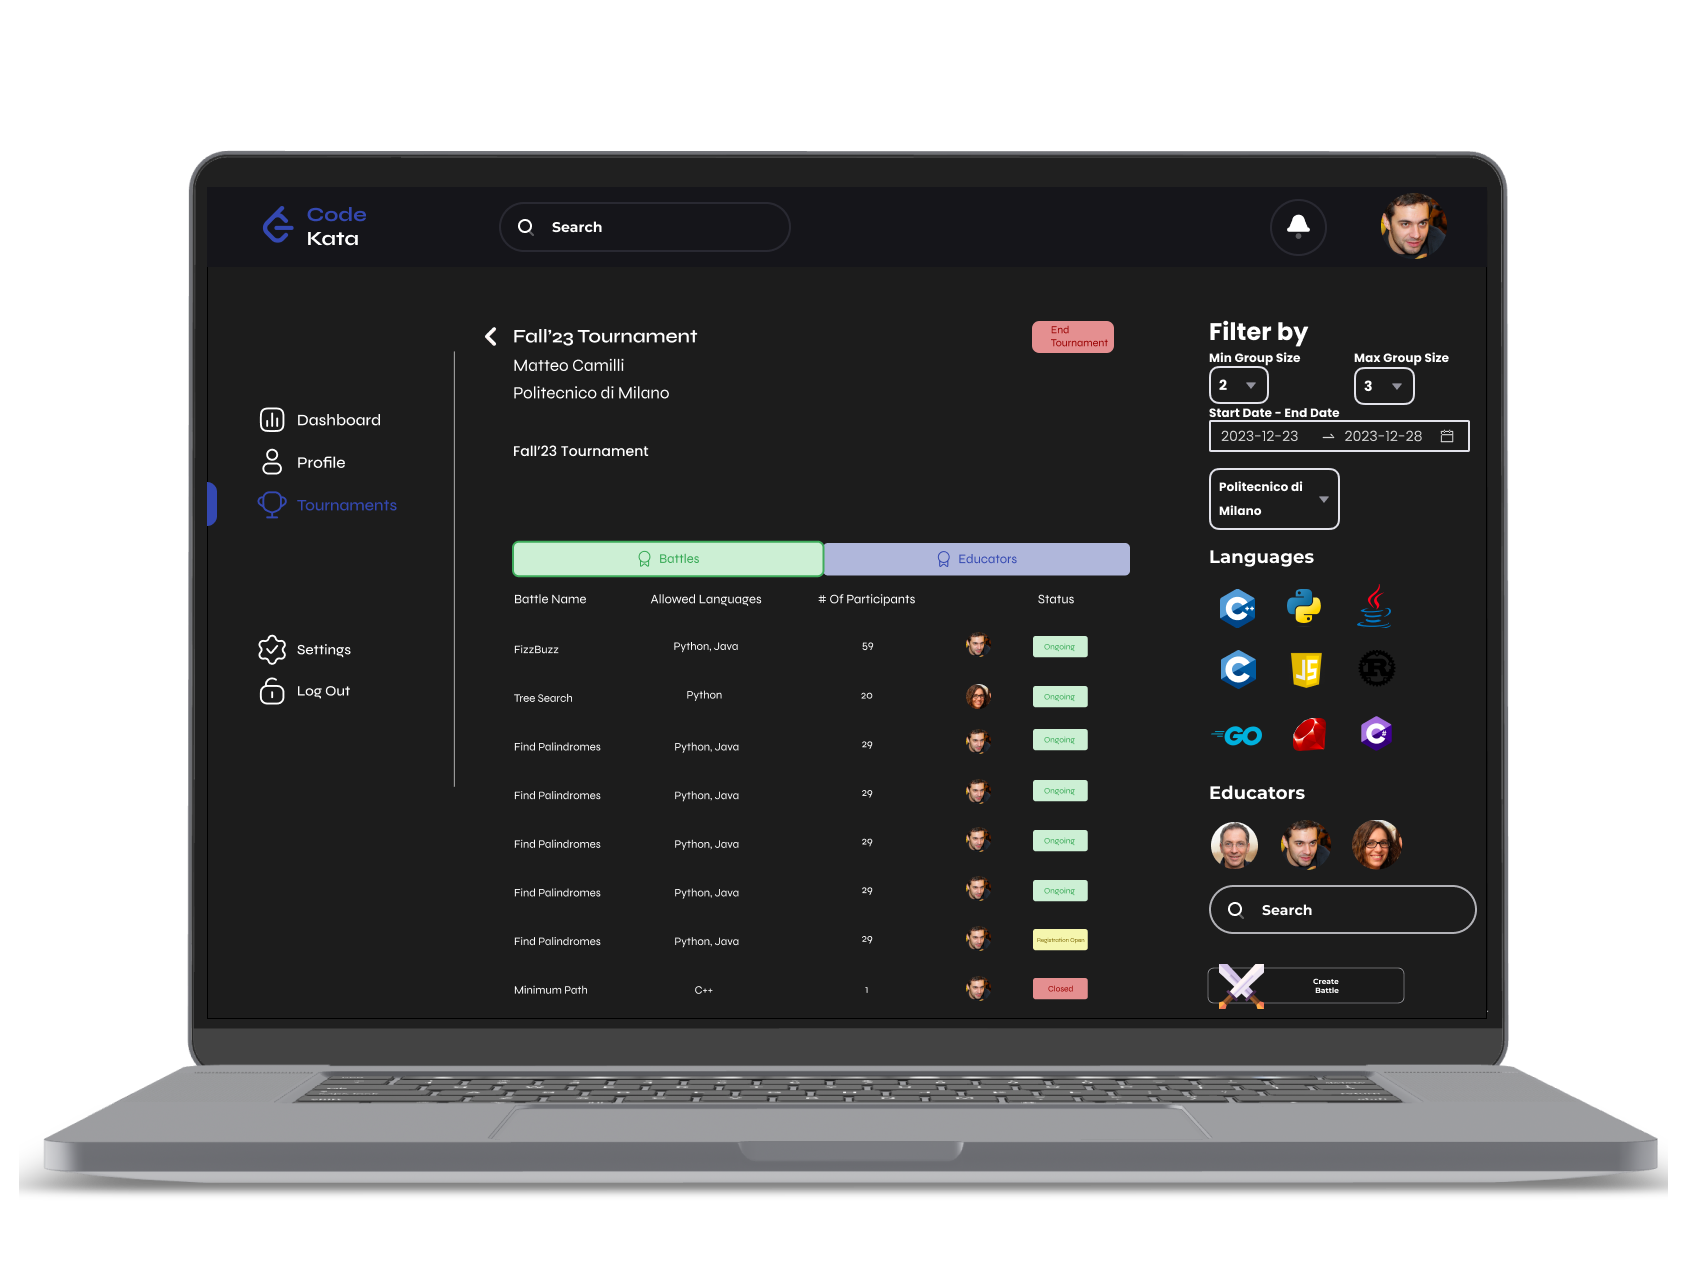
\includegraphics[scale=0.13]{Images/ui-ux/educator_creates_battle_1.png}
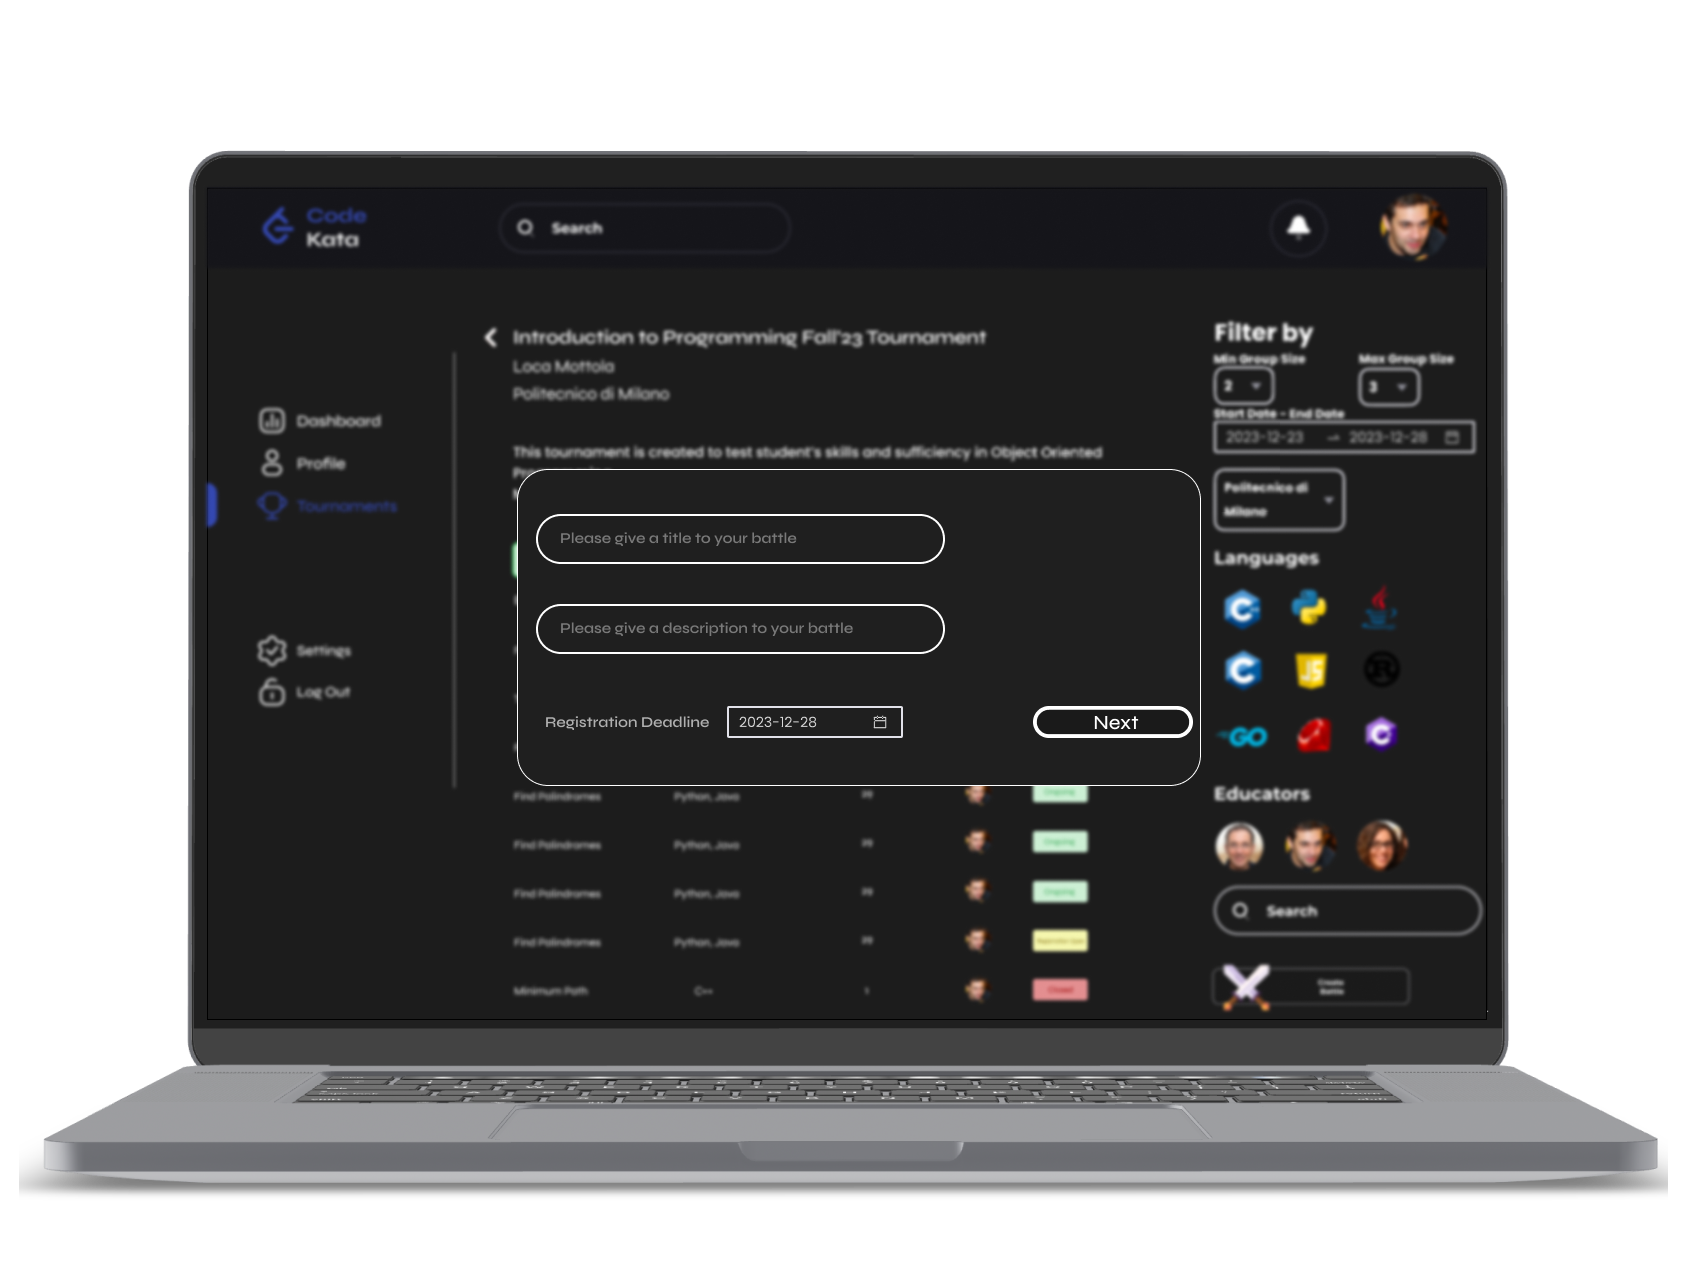
\includegraphics[scale=0.13]{Images/ui-ux/educator_creates_battle_2.png}
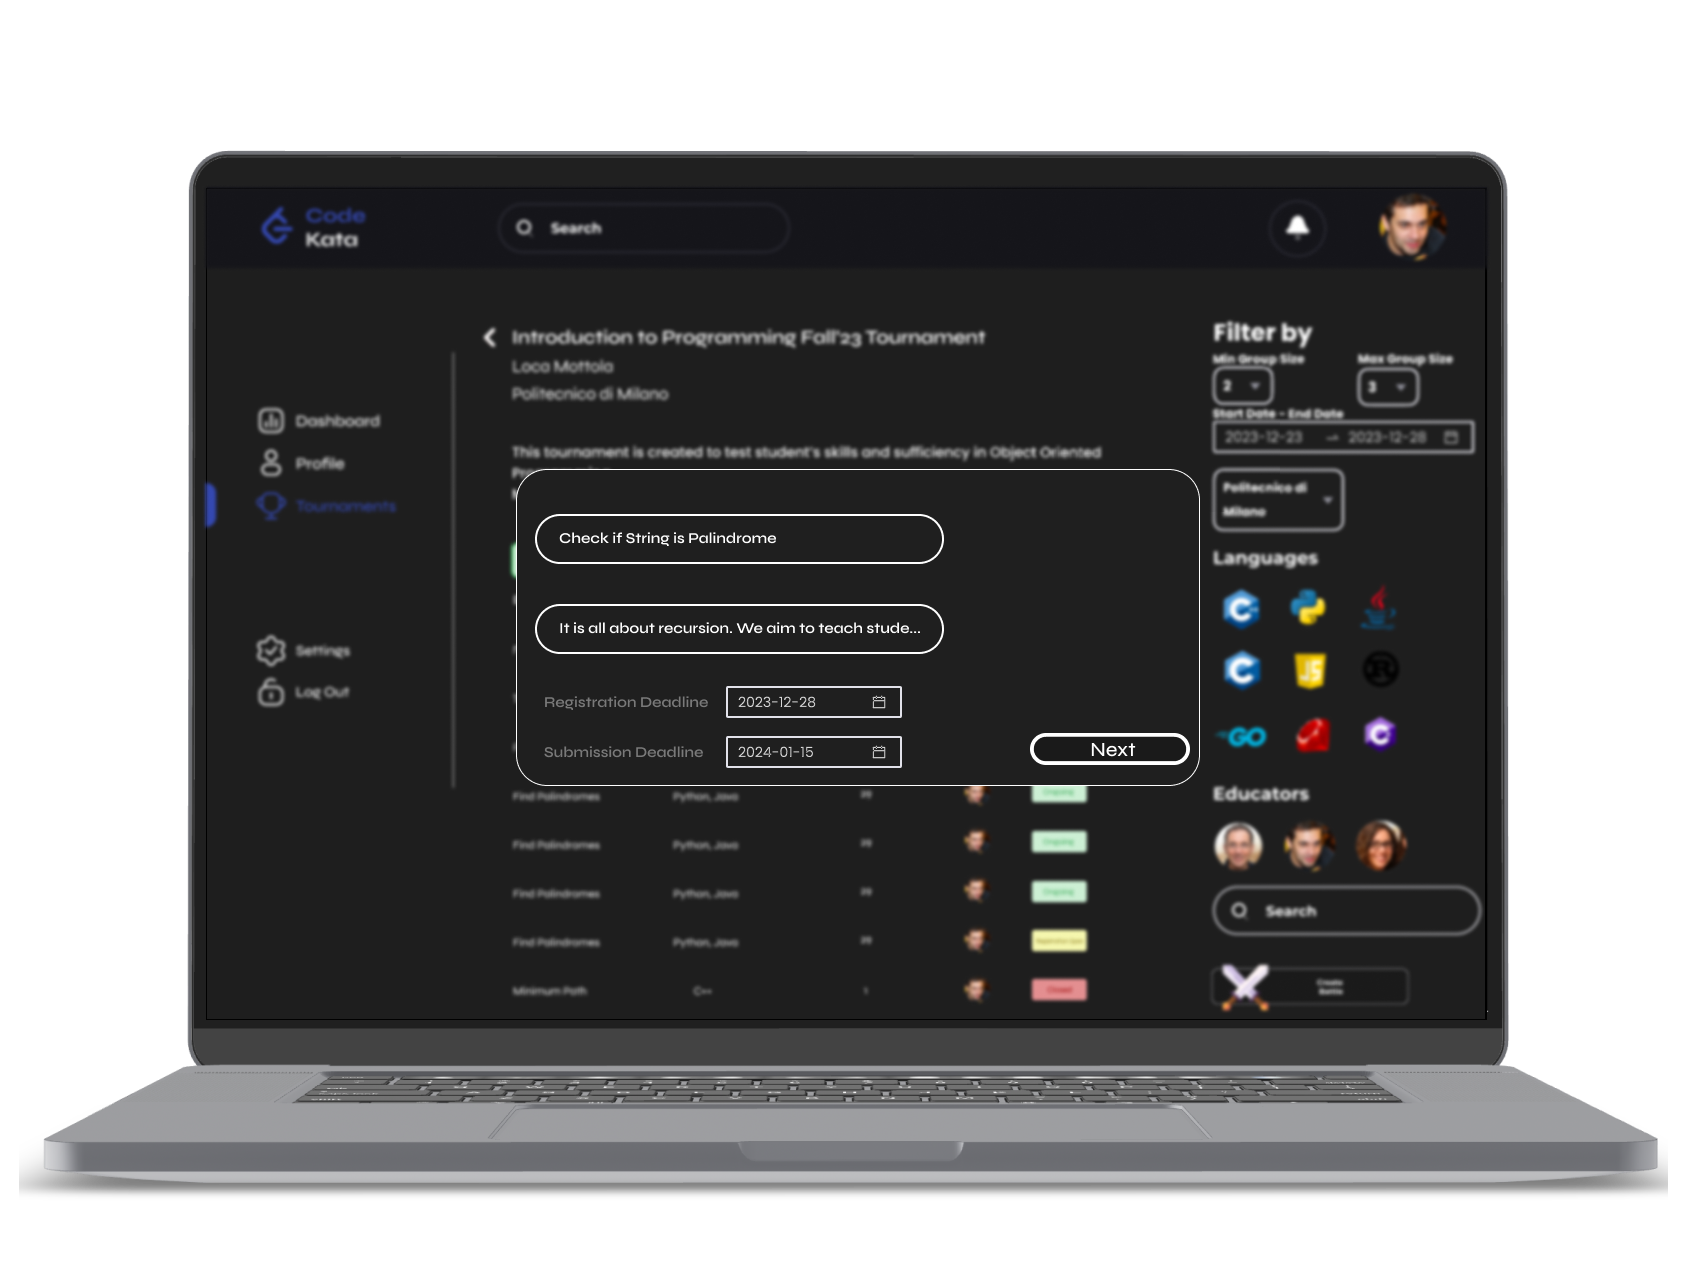
\includegraphics[scale=0.13]{Images/ui-ux/educator_creates_battle_3.png}
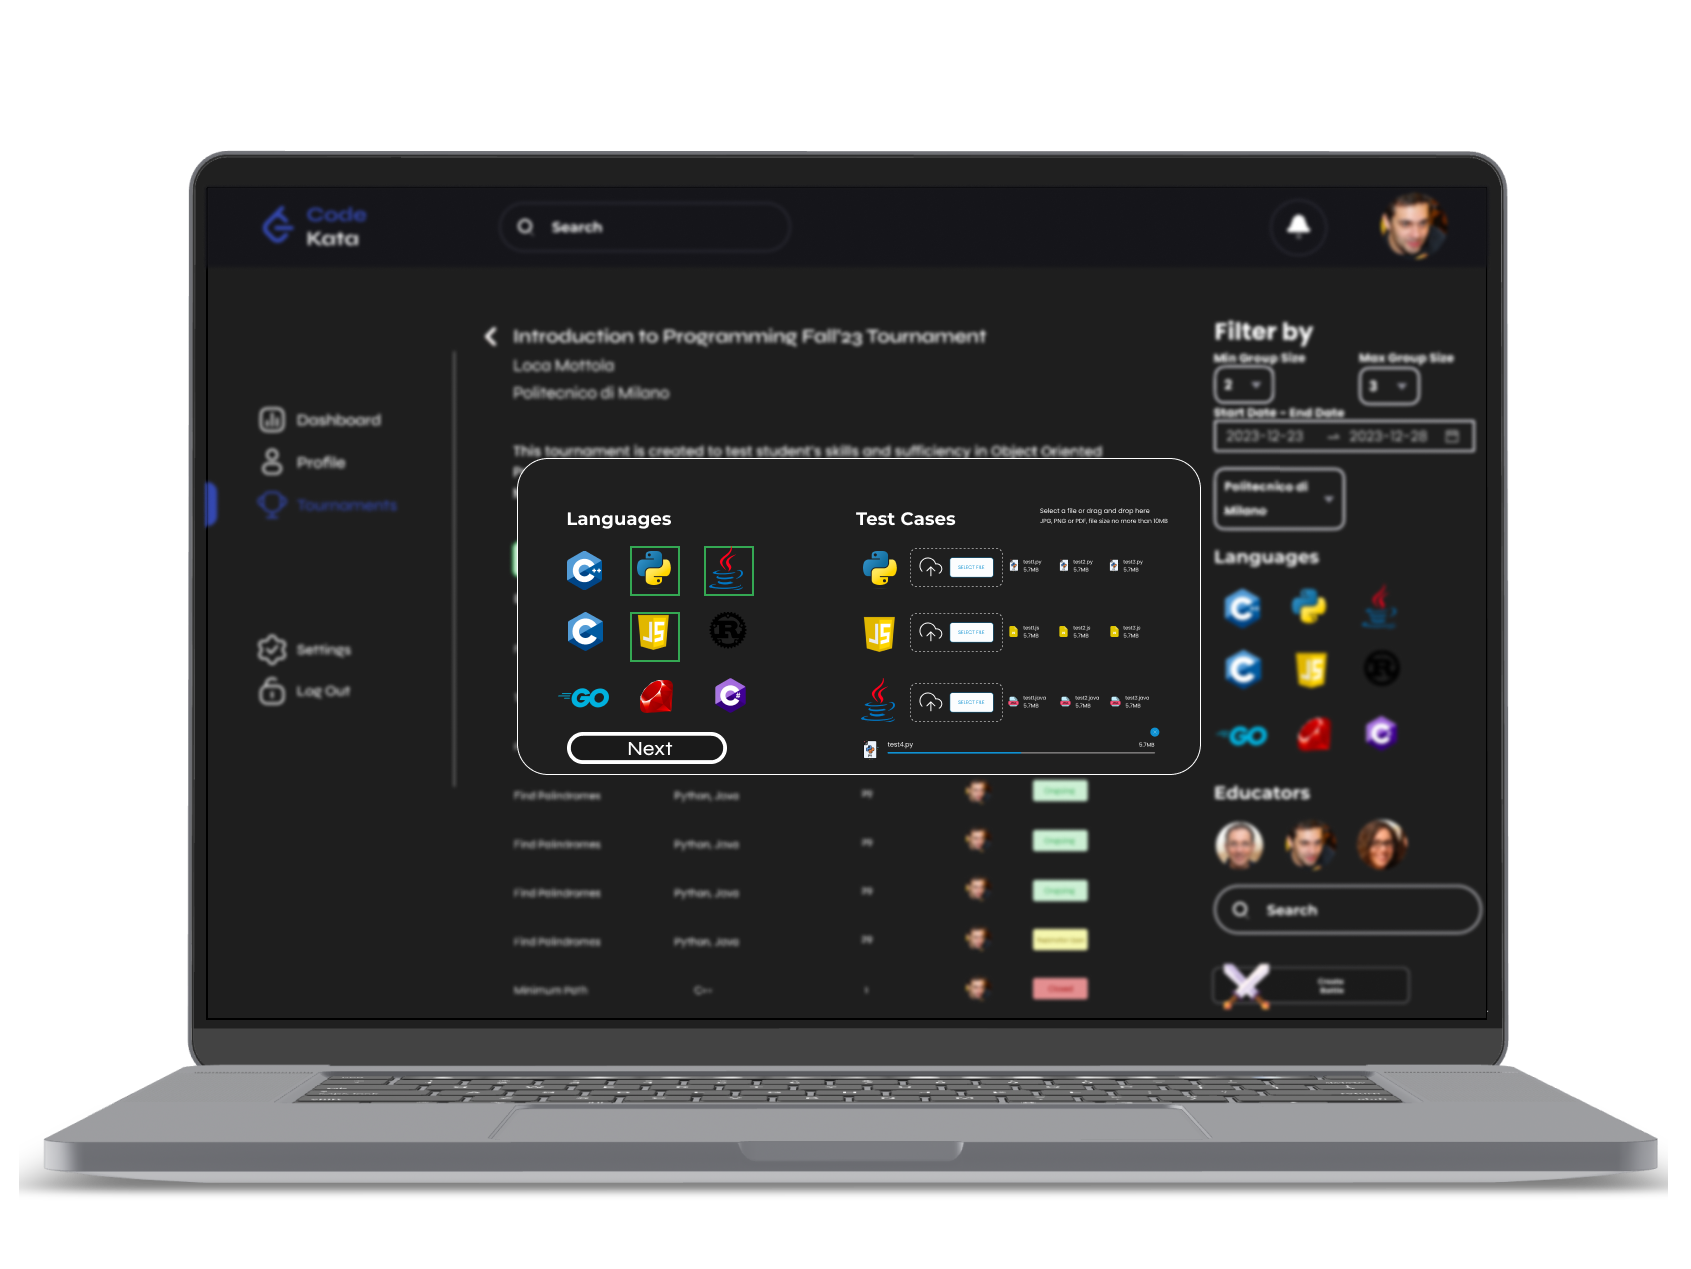
\includegraphics[scale=0.13]{Images/ui-ux/educator_creates_battle_4.png}
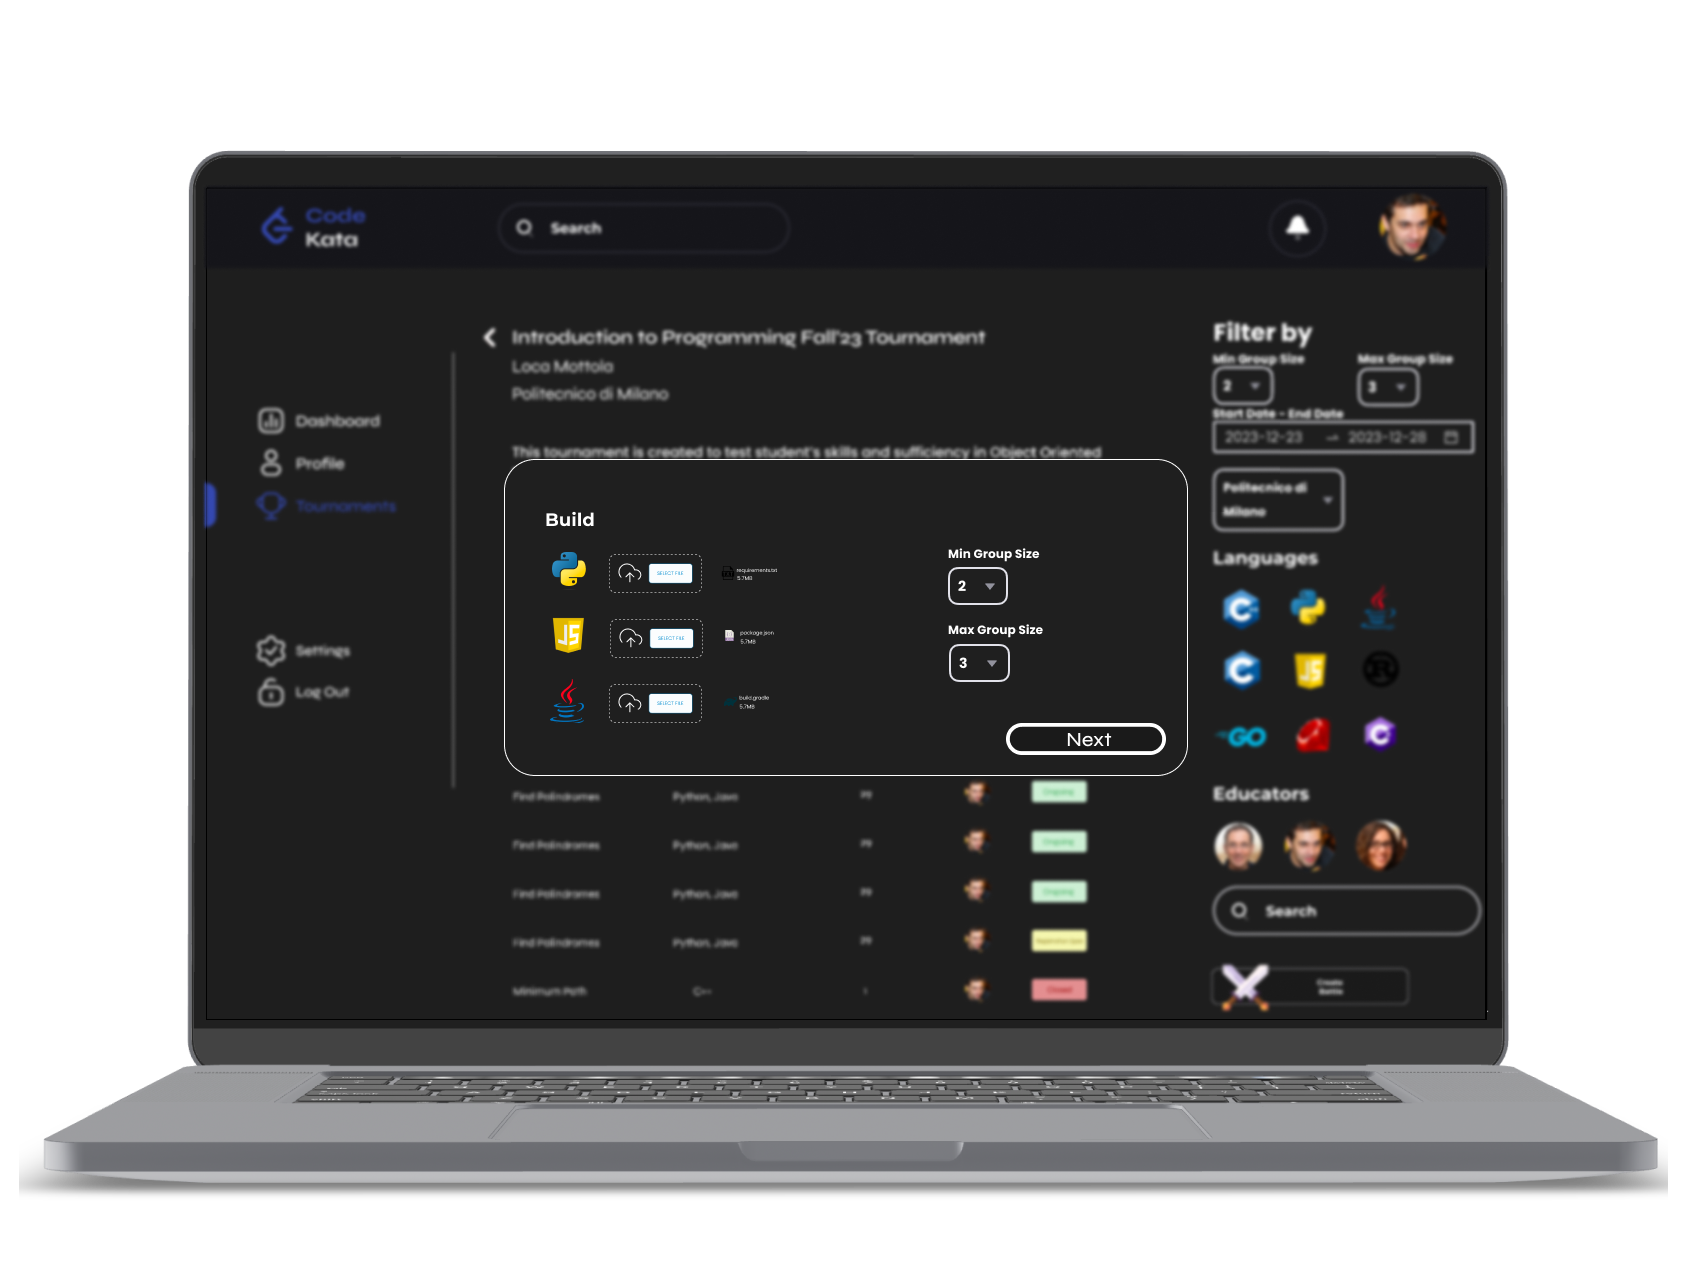
\includegraphics[scale=0.13]{Images/ui-ux/educator_creates_battle_5.png}
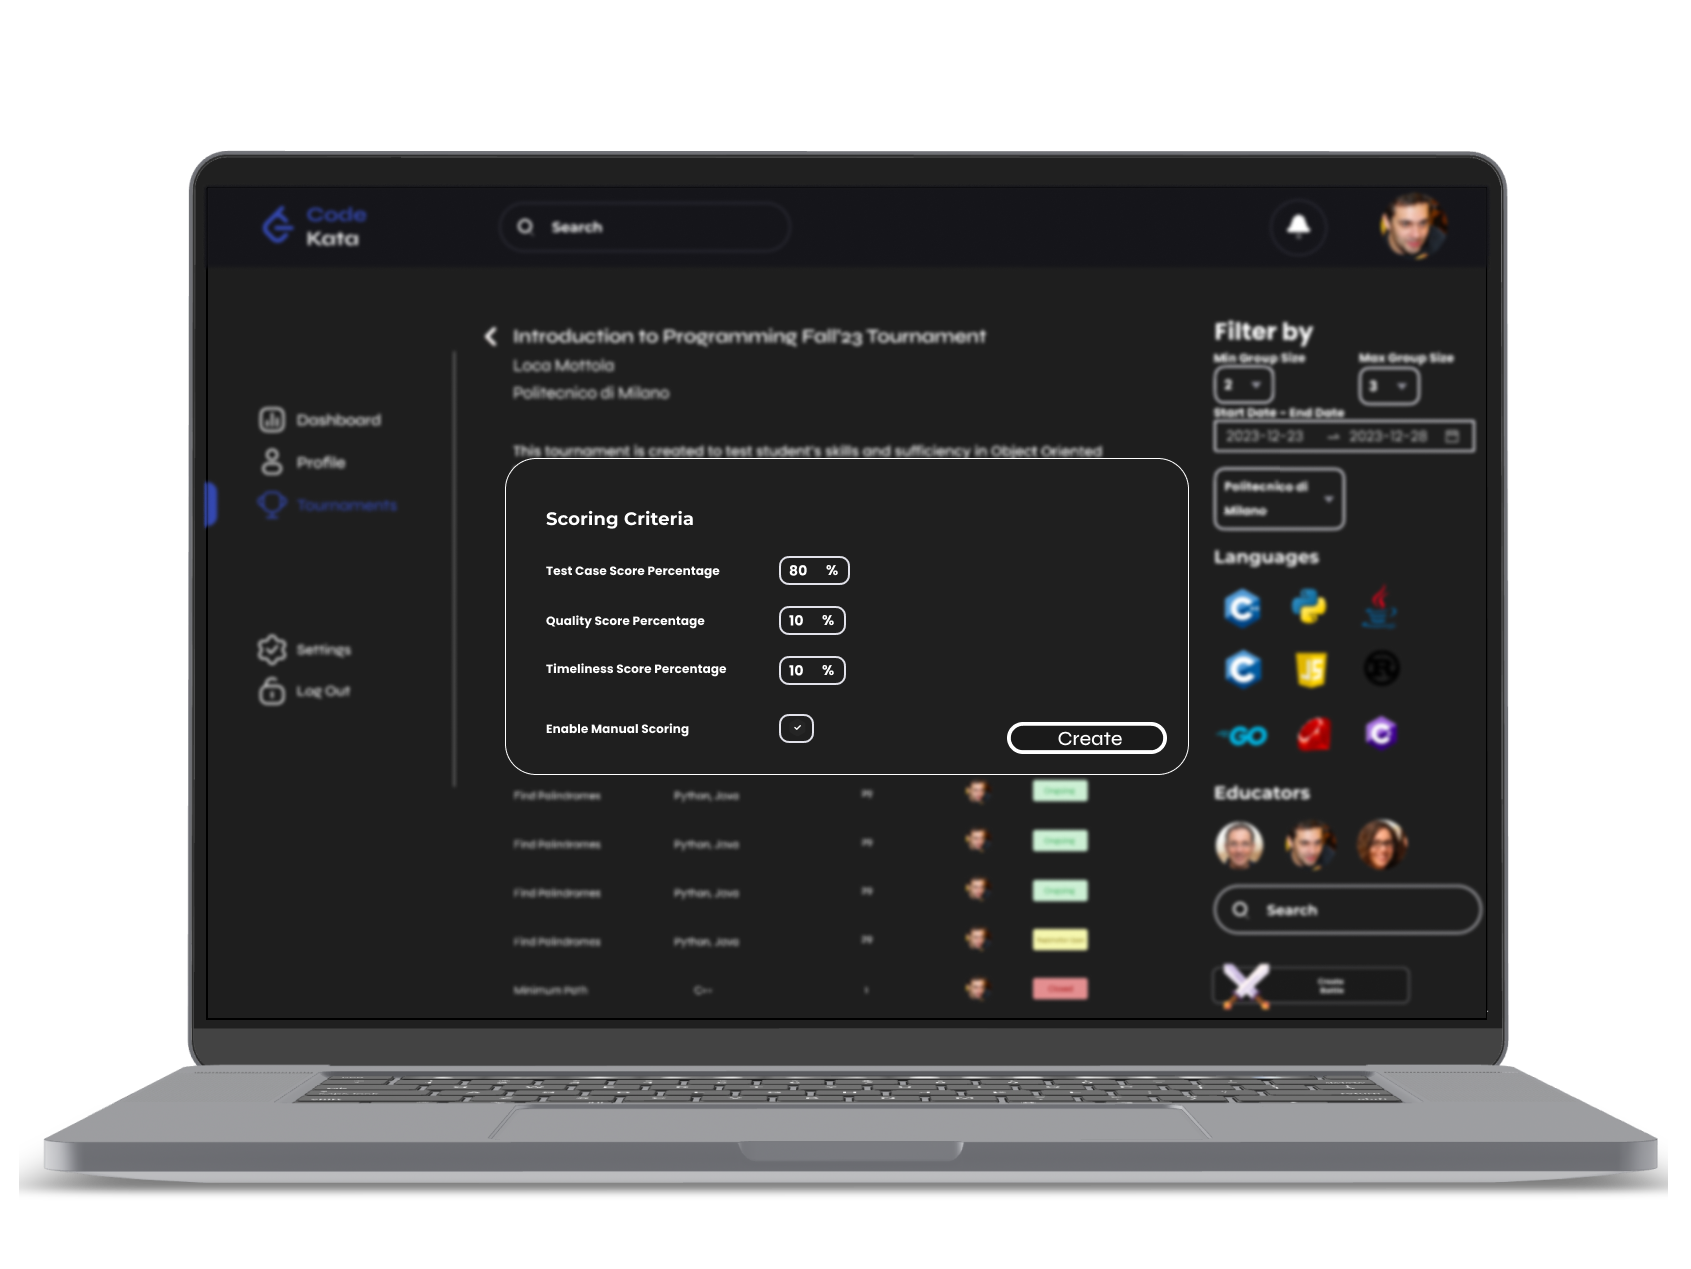
\includegraphics[scale=0.13]{Images/ui-ux/educator_creates_battle_6.png}
        (l) $UI_{12}$ Educator Creates Battle
\end{center}
\newpage
\begin{center}
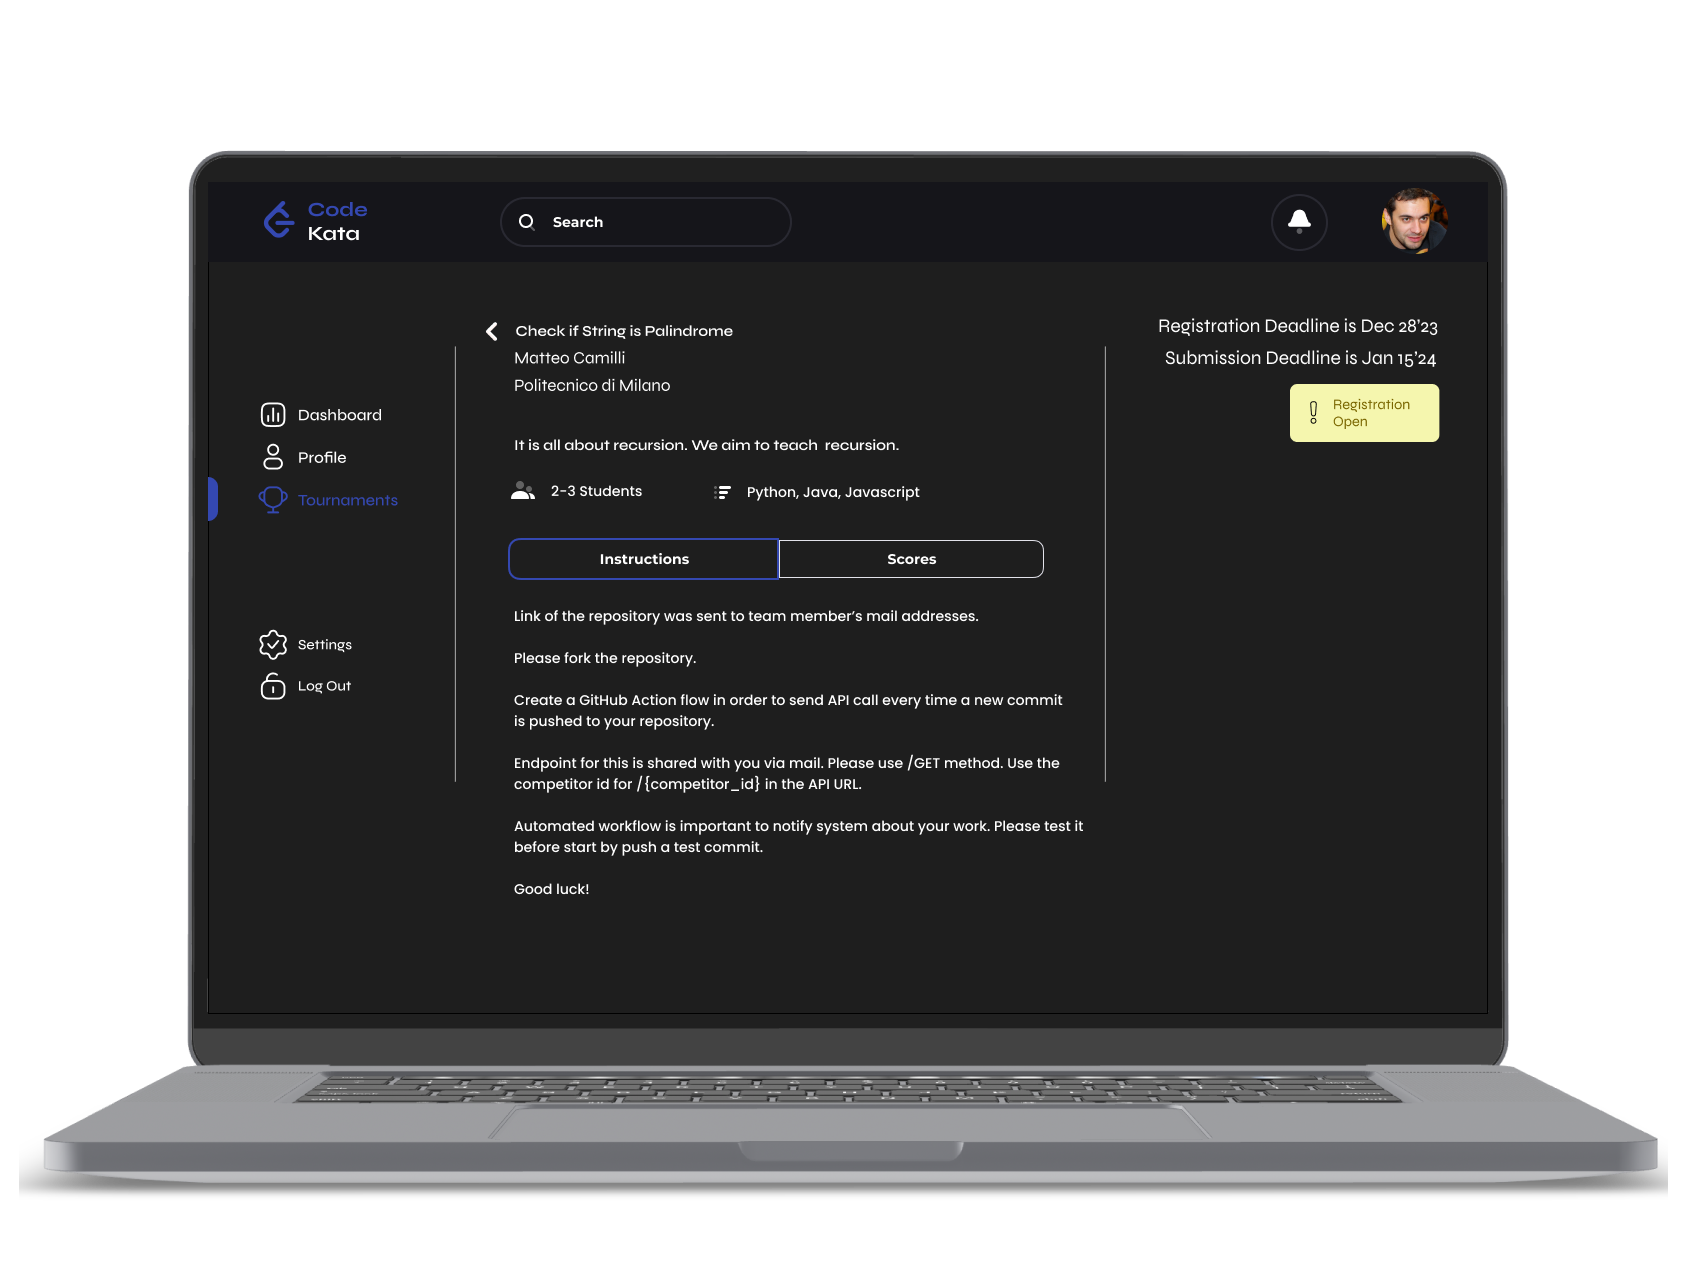
\includegraphics[scale=0.13]{Images/ui-ux/educator_battle_1.png}
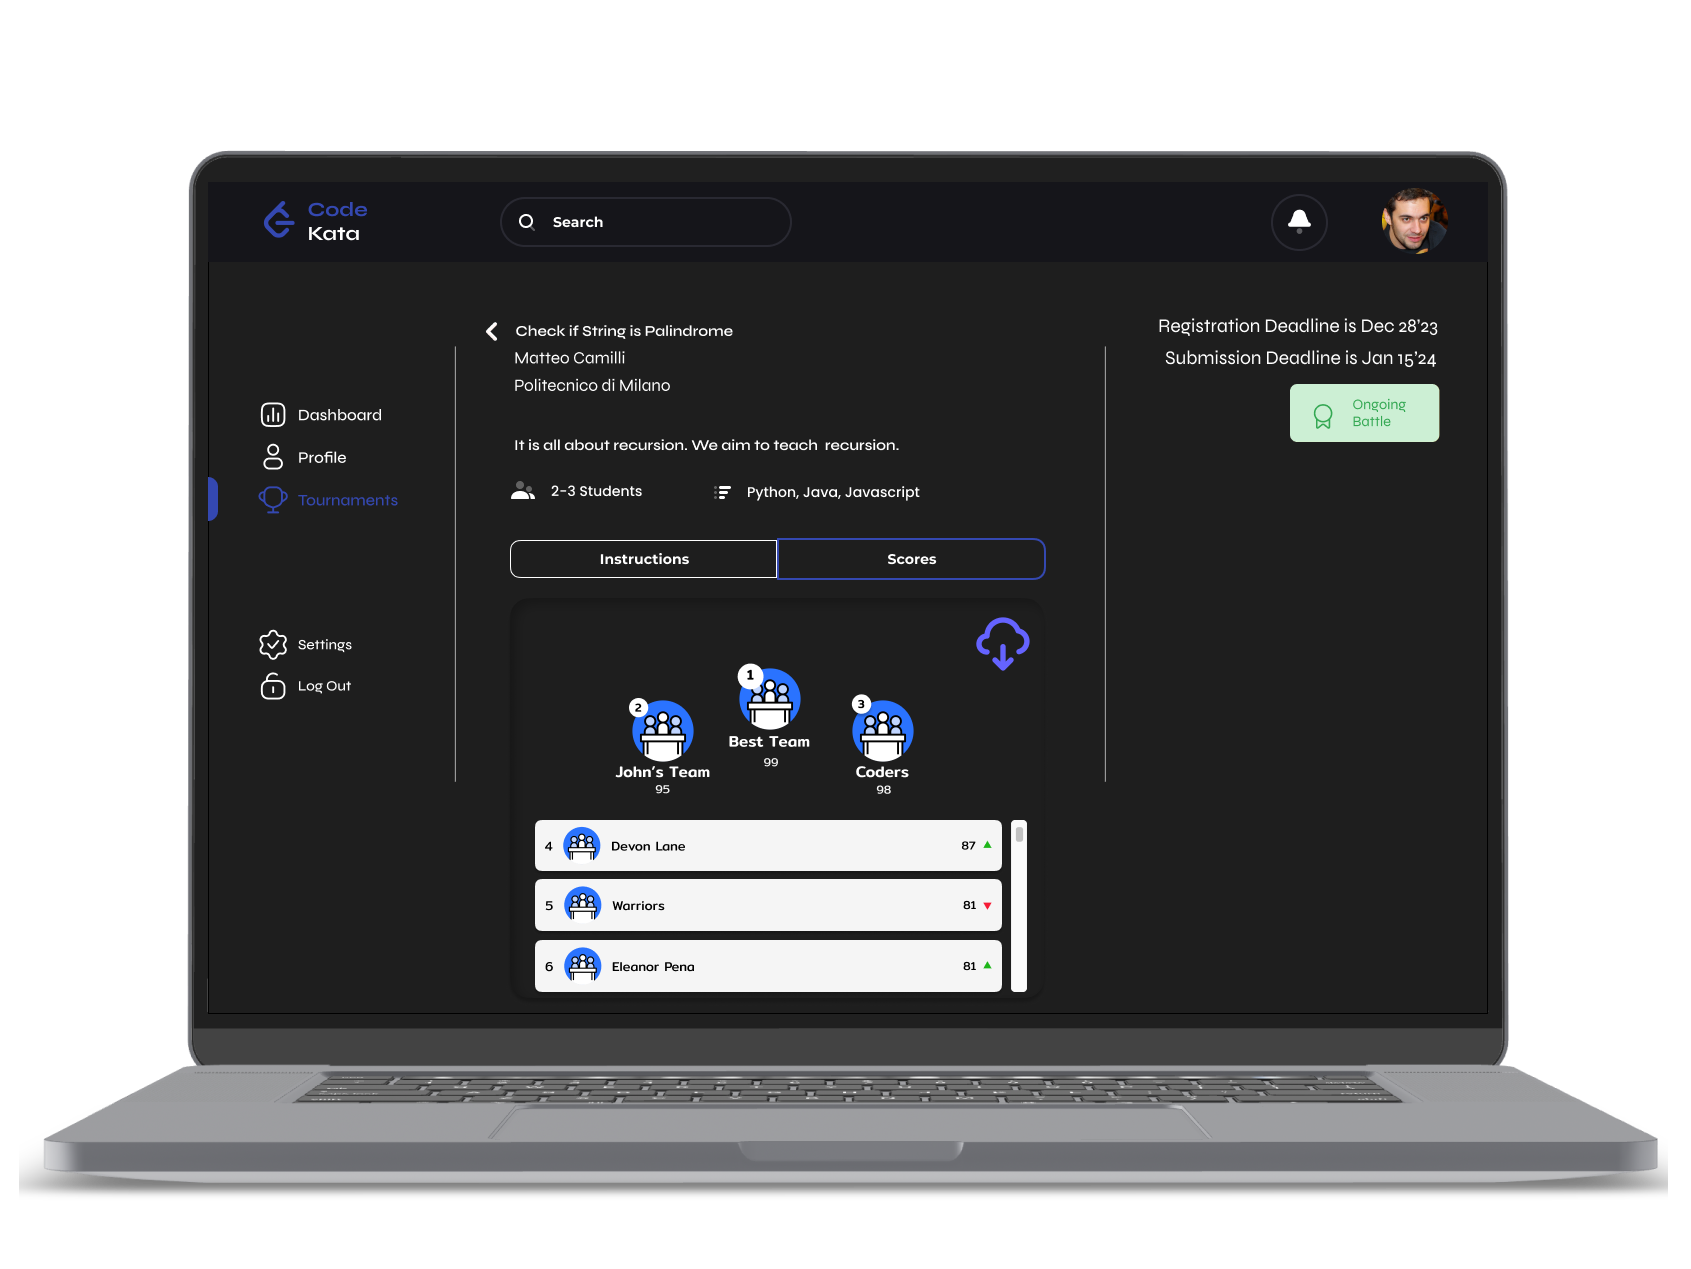
\includegraphics[scale=0.13]{Images/ui-ux/educator_battle_2.png}
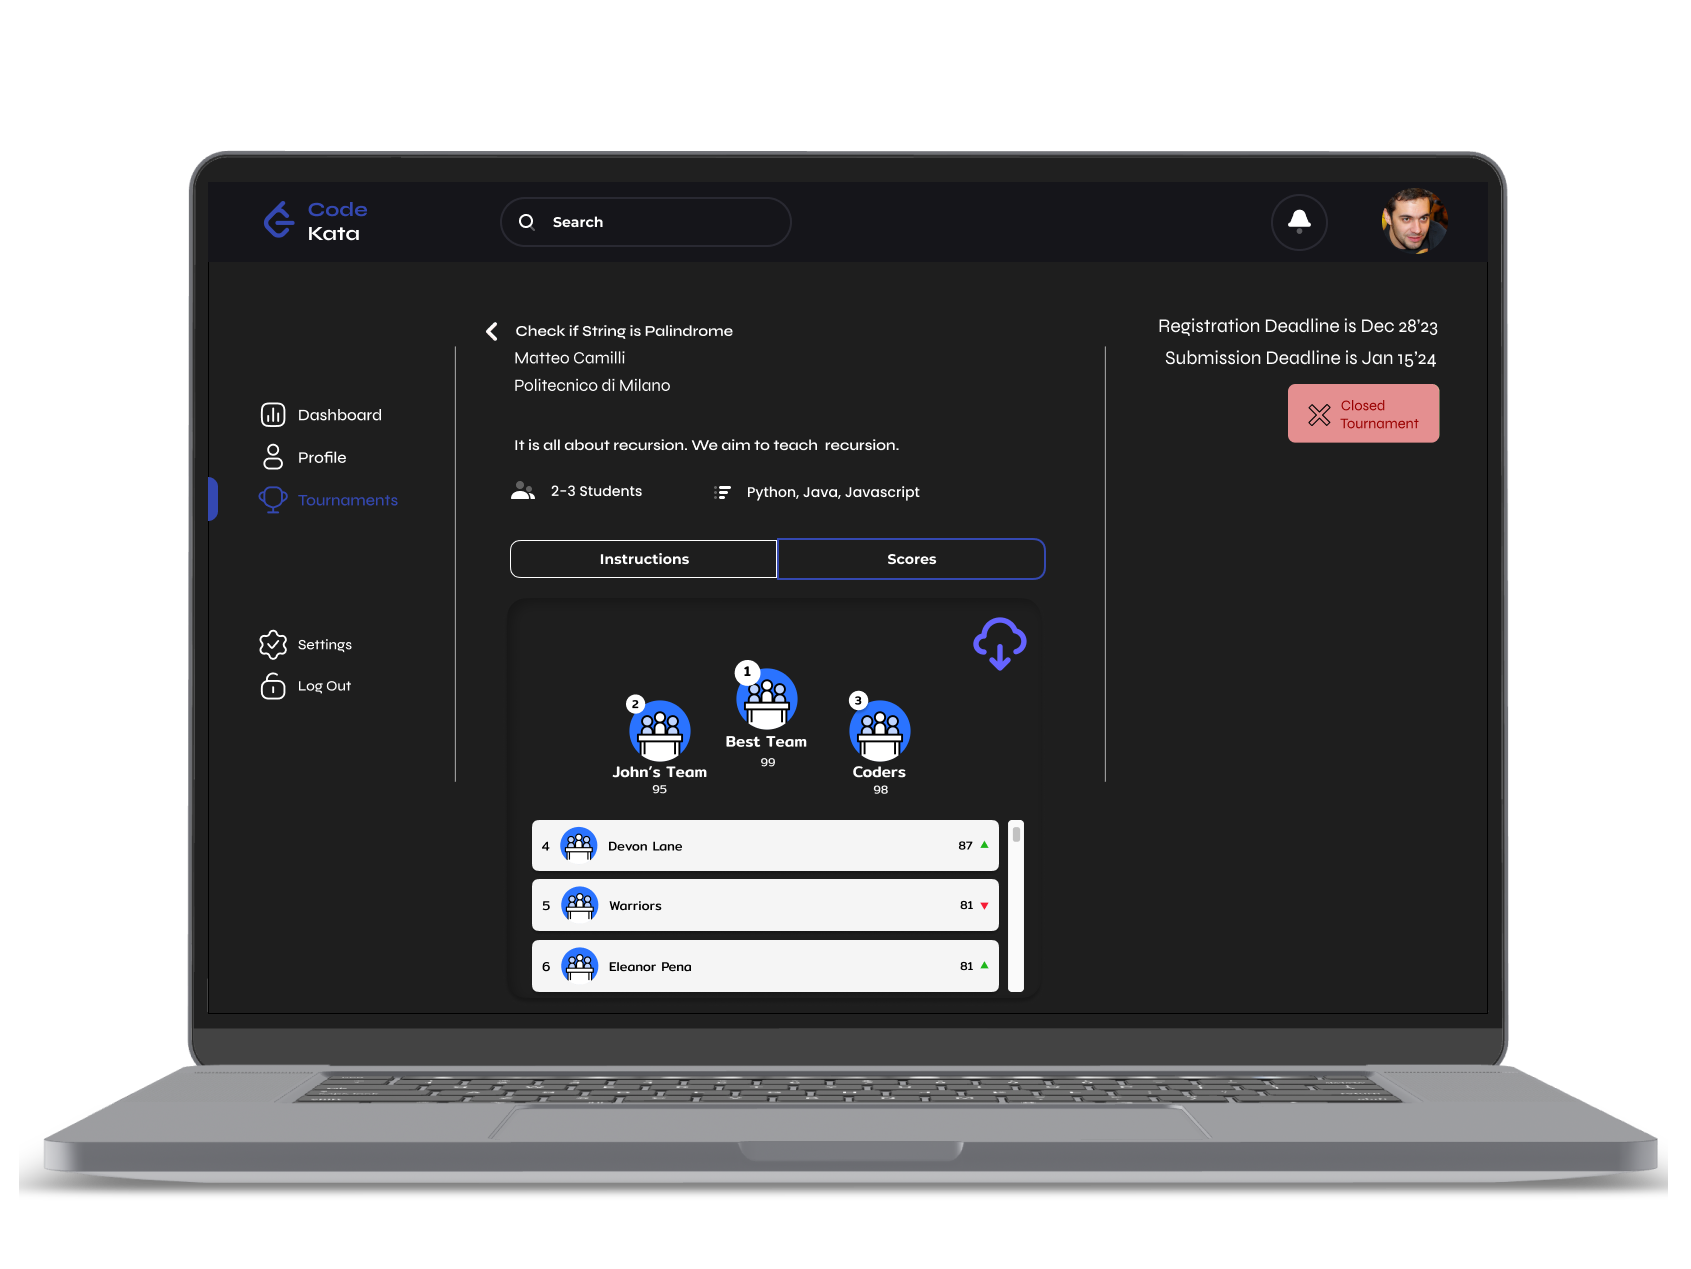
\includegraphics[scale=0.13]{Images/ui-ux/educator_battle_3.png}
\\ (m) $UI_{13}$  Educator visits Battle
\end{center}
\newpage
\begin{center}
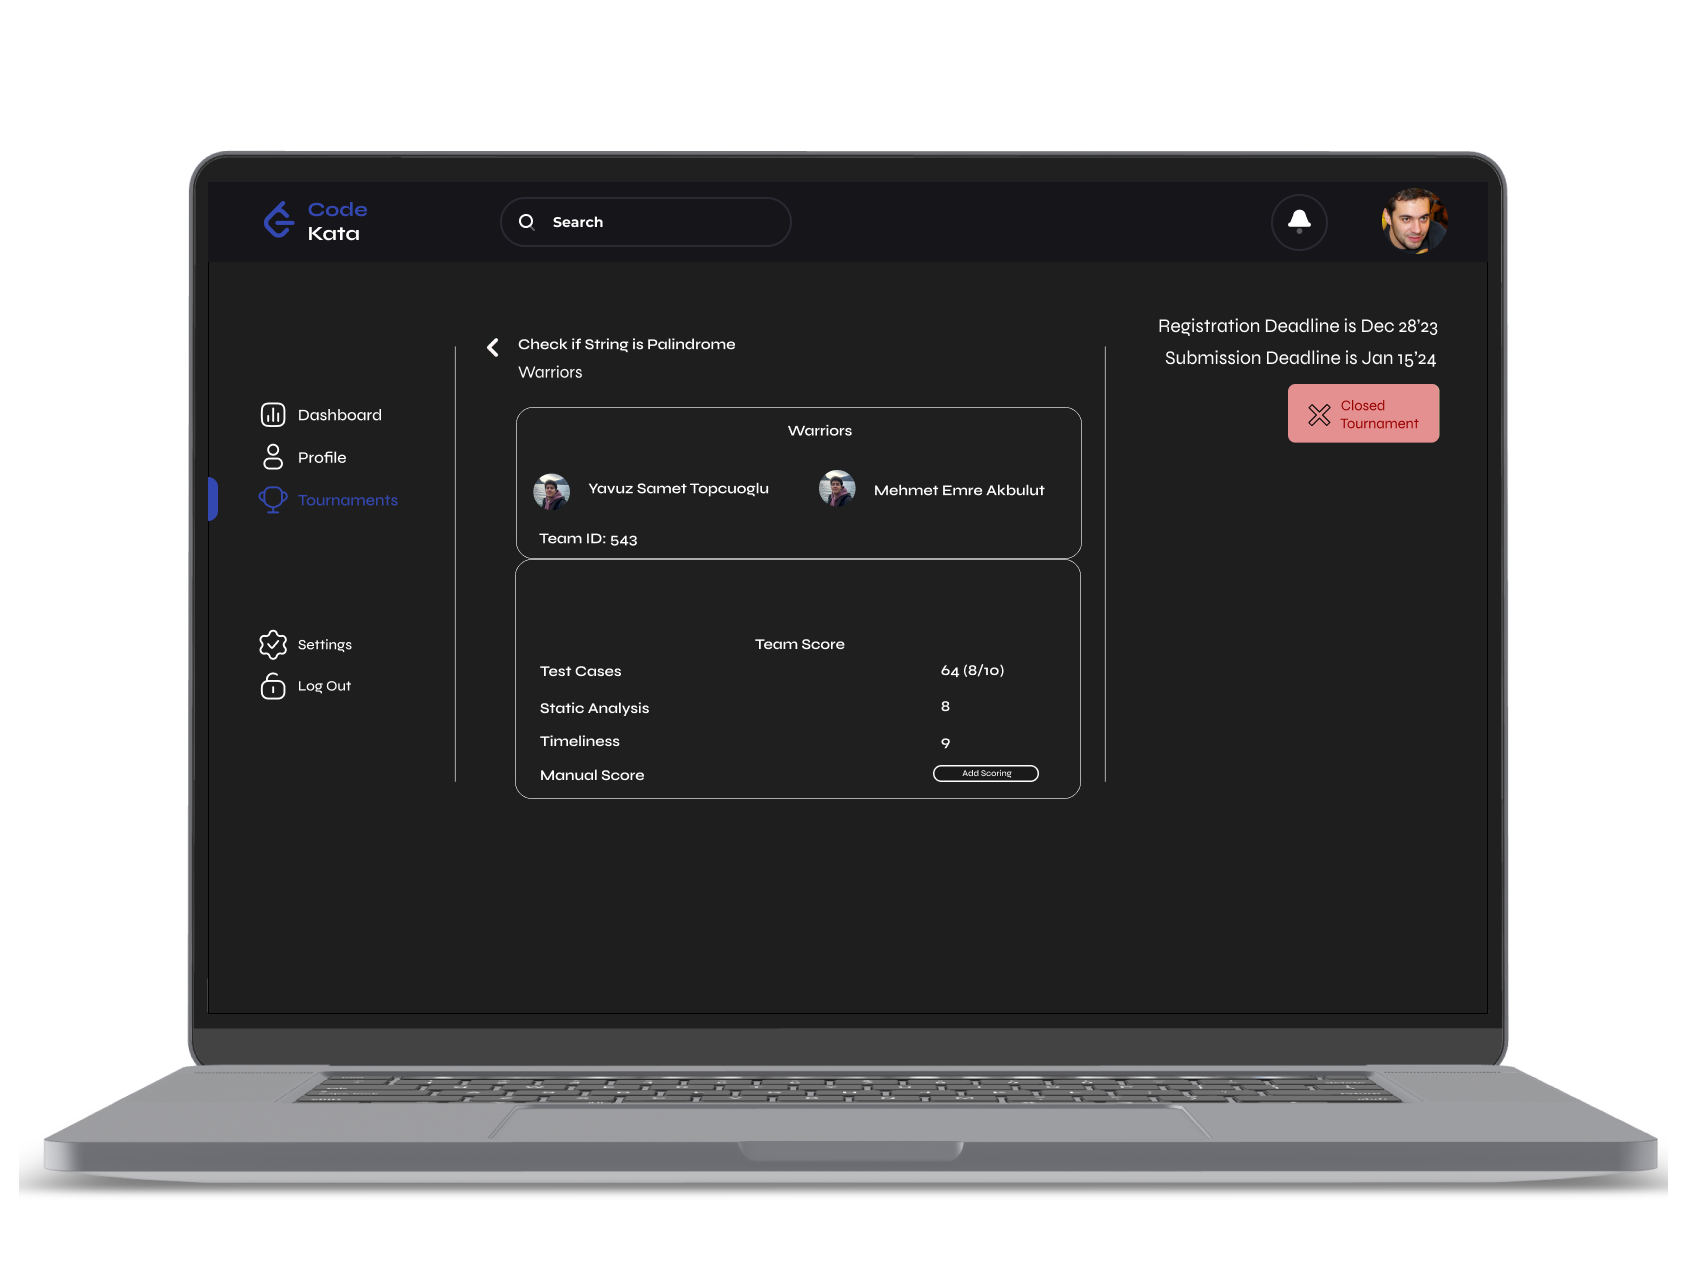
\includegraphics[scale=0.13]{Images/ui-ux/educator_team_1 (1).png}
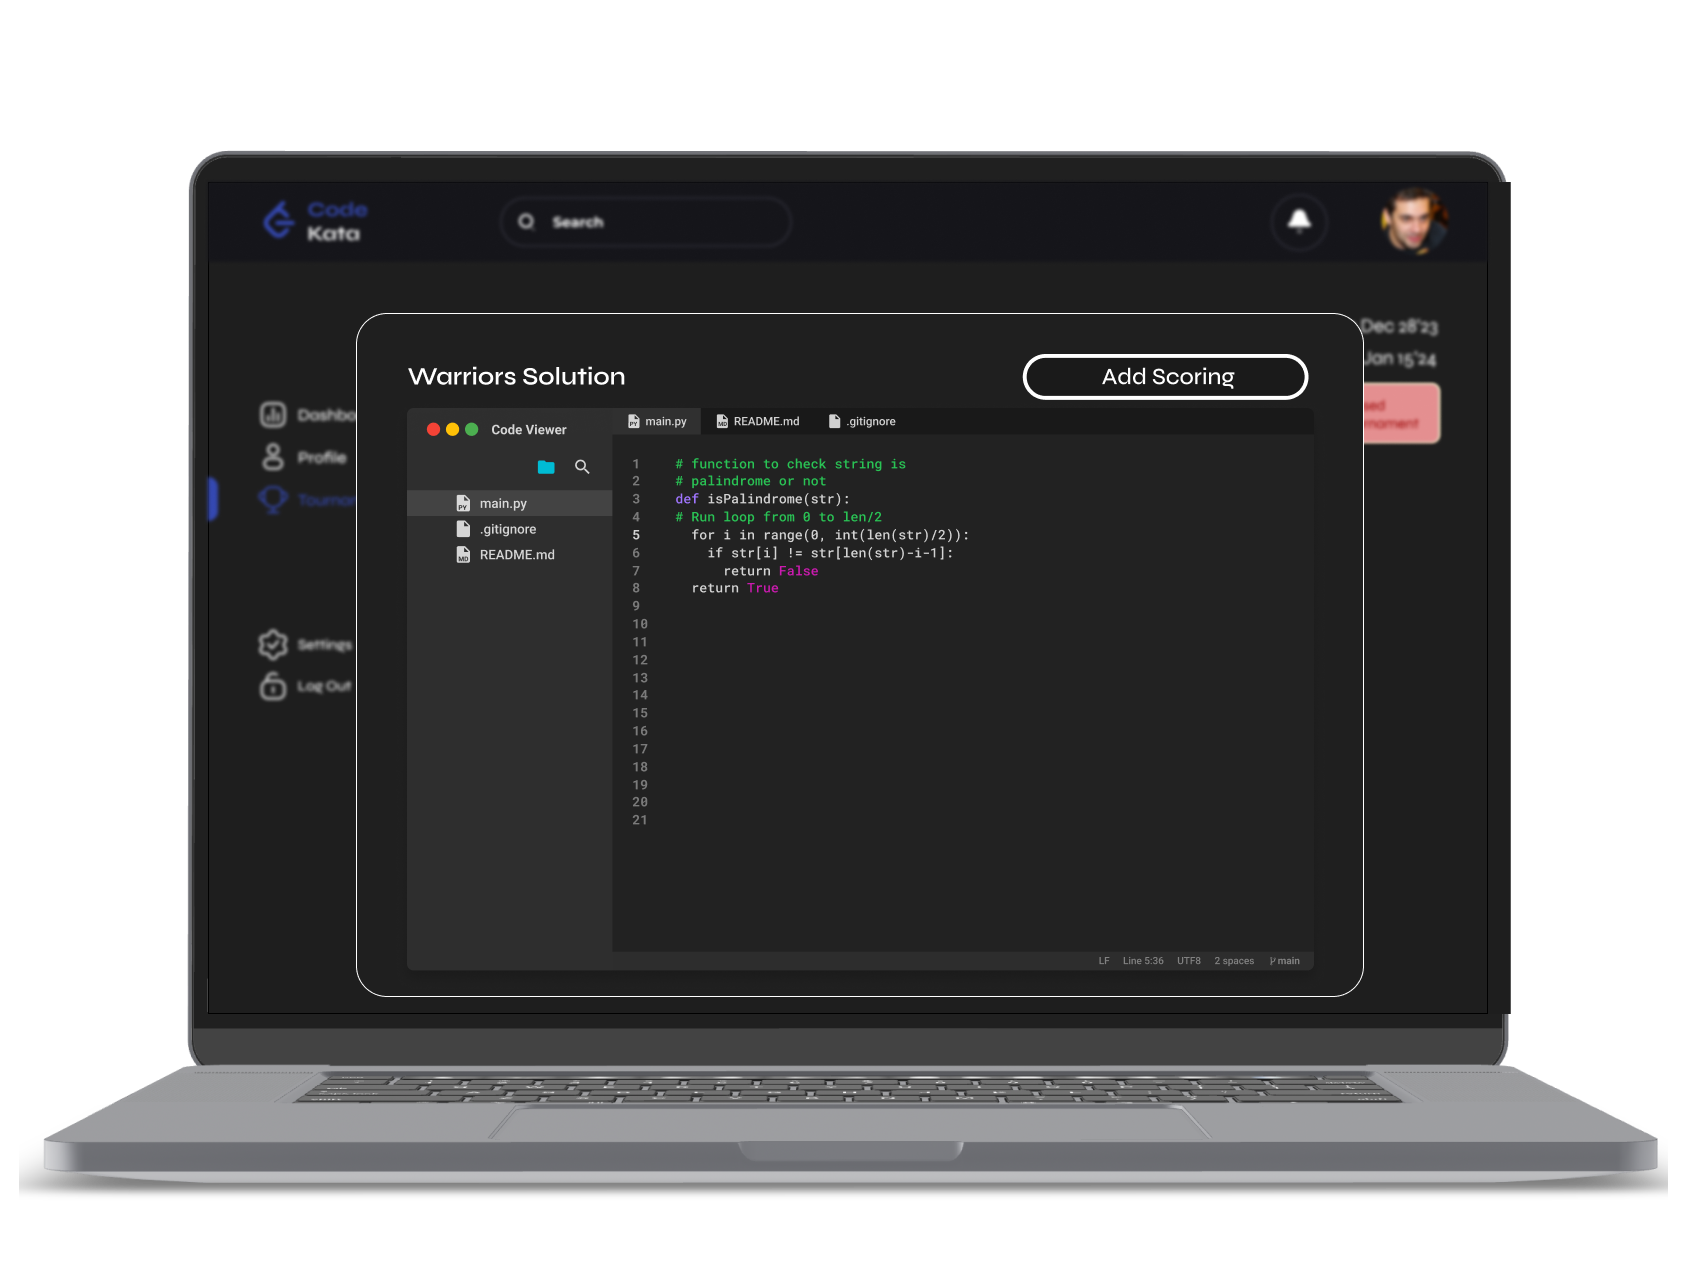
\includegraphics[scale=0.13]{Images/ui-ux/educator_team_2 (1).png}
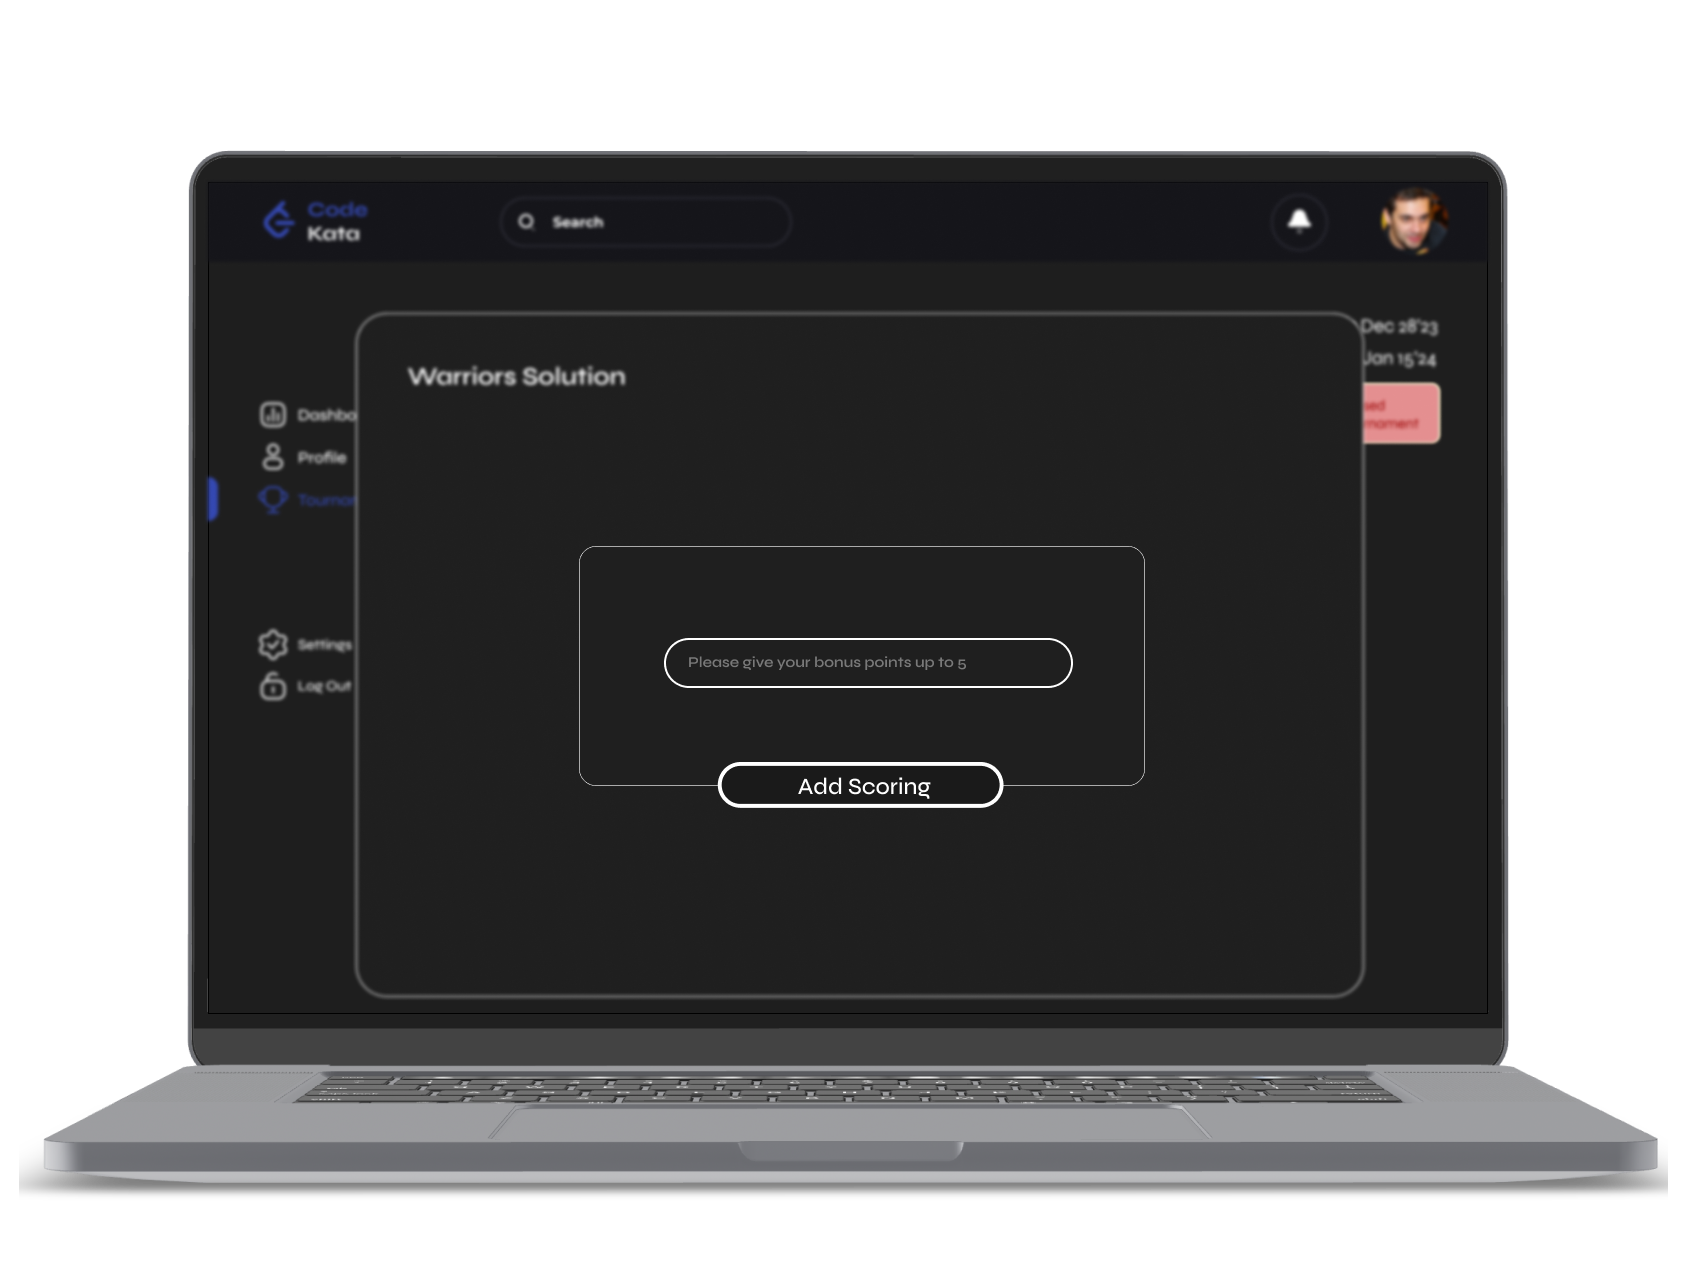
\includegraphics[scale=0.13]{Images/ui-ux/educator_team_3 (1).png}
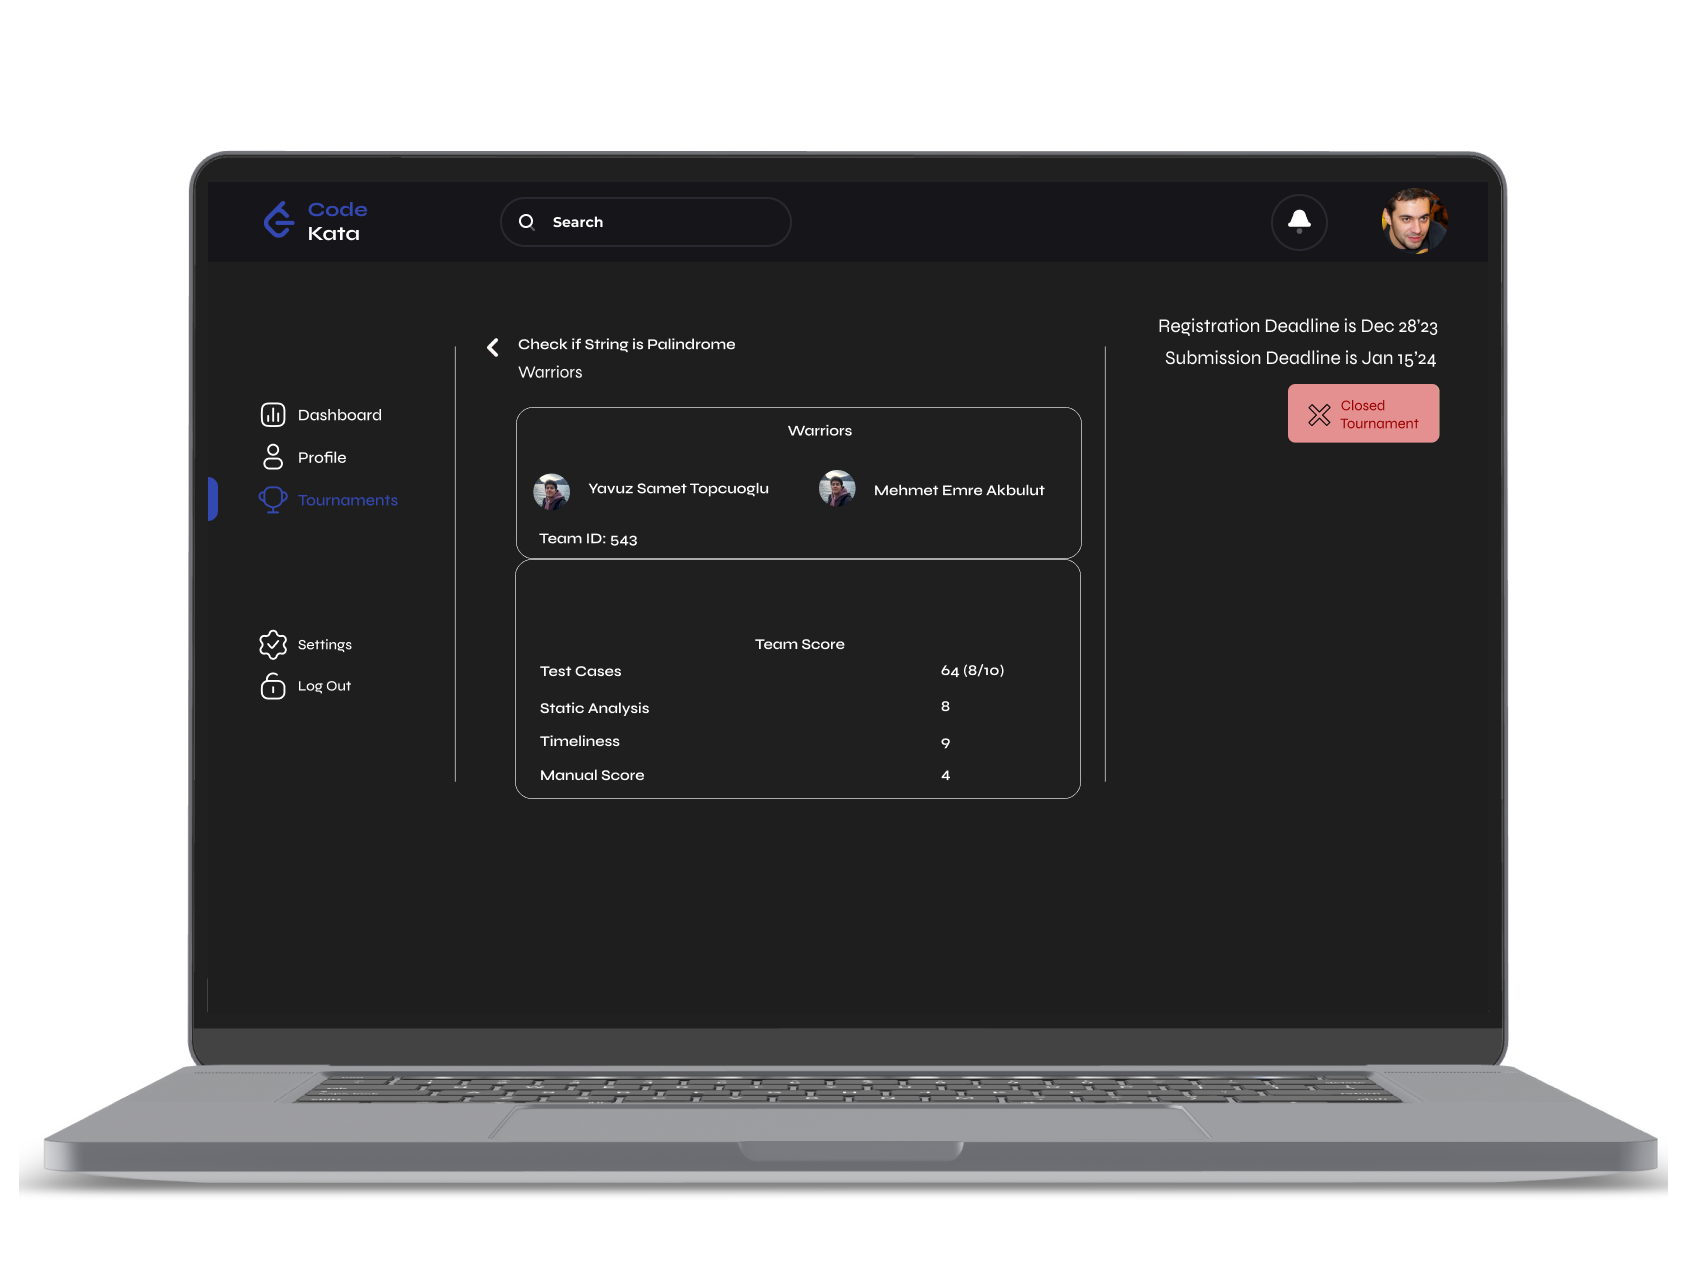
\includegraphics[scale=0.13]{Images/ui-ux/educator_team_4 (1).png}
        (n) $UI_{14}$  Educator, Team and Manual Scoring
\end{center}
\begin{center}
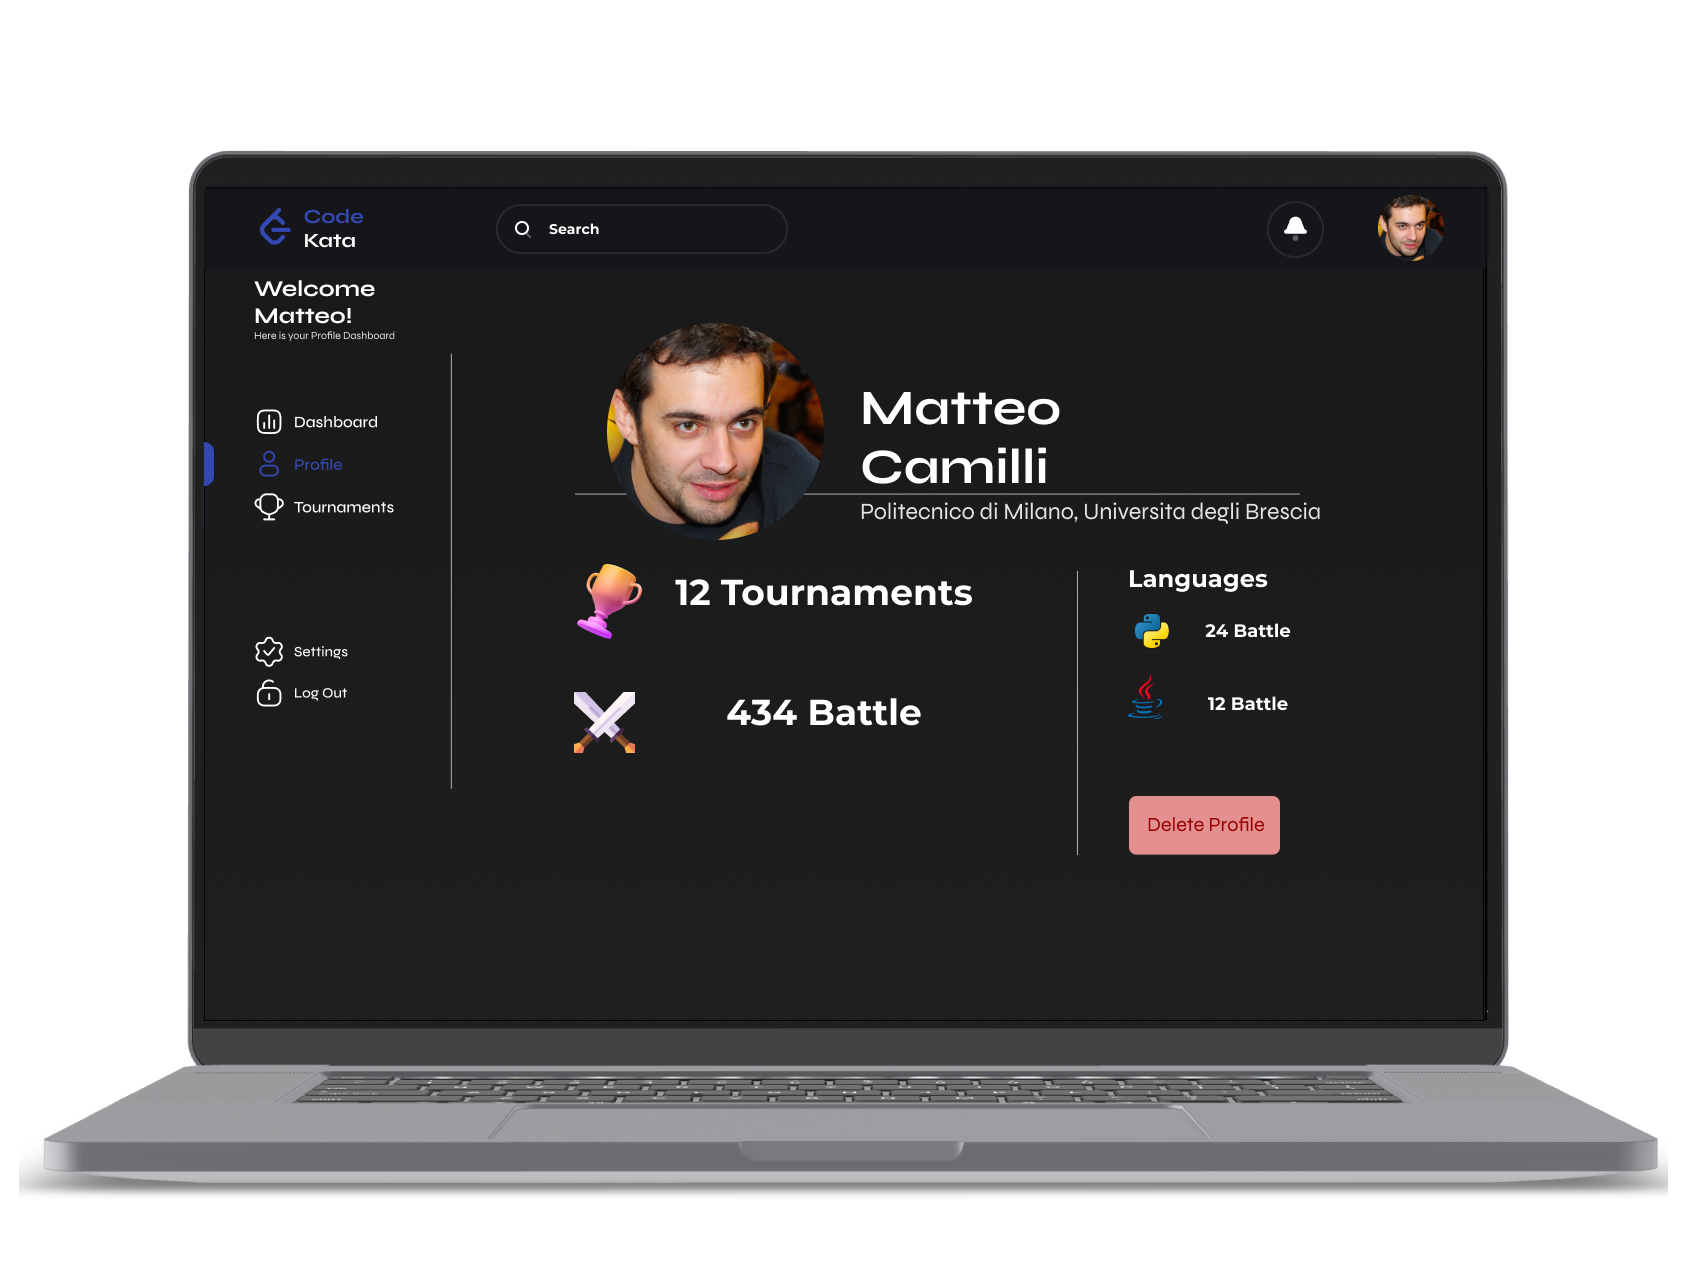
\includegraphics[scale=0.13]{Images/ui-ux/educator_profile.png}
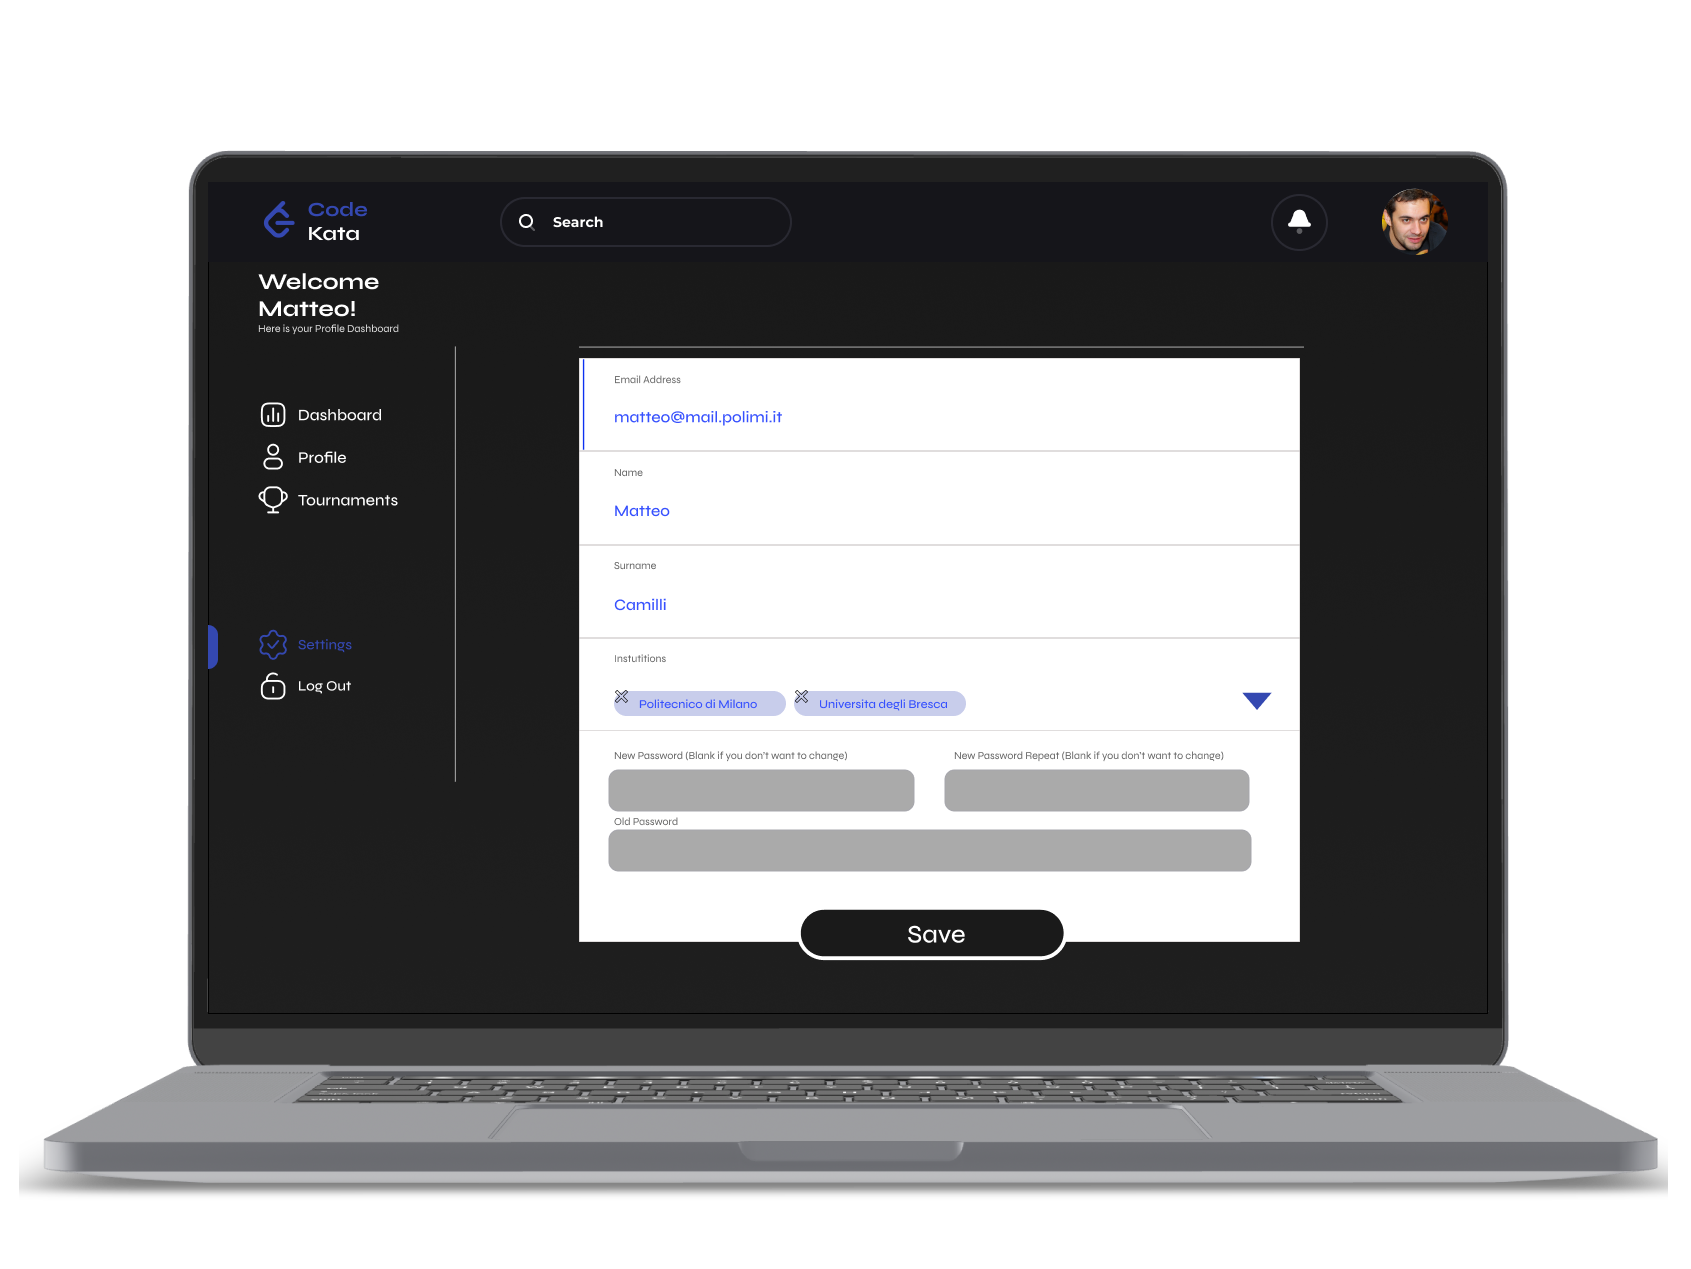
\includegraphics[scale=0.13]{Images/ui-ux/educator_settings.png}
        (o) $UI_{15}$  Educator Profile and Settings
\end{center}
\newpage
\begin{center}
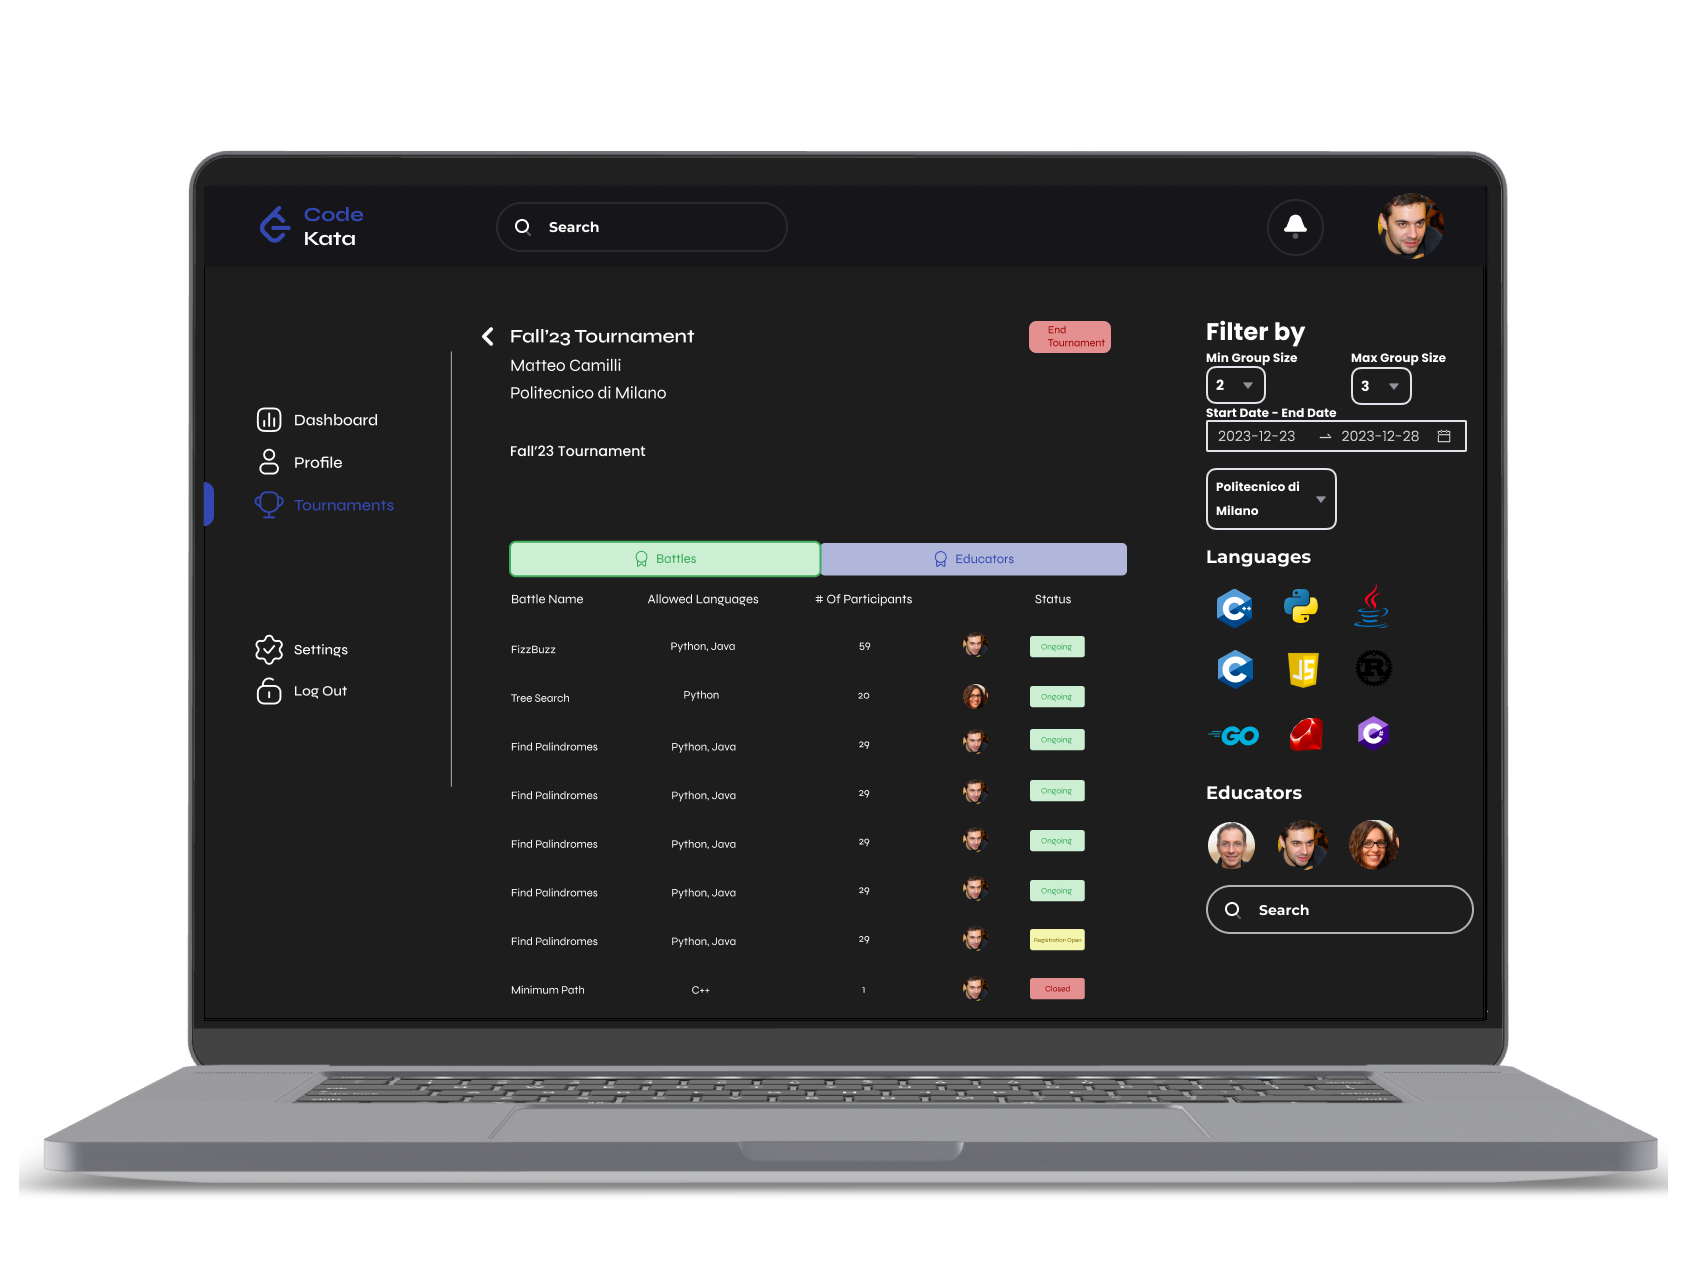
\includegraphics[scale=0.13]{Images/ui-ux/educator_end_tournament.png}
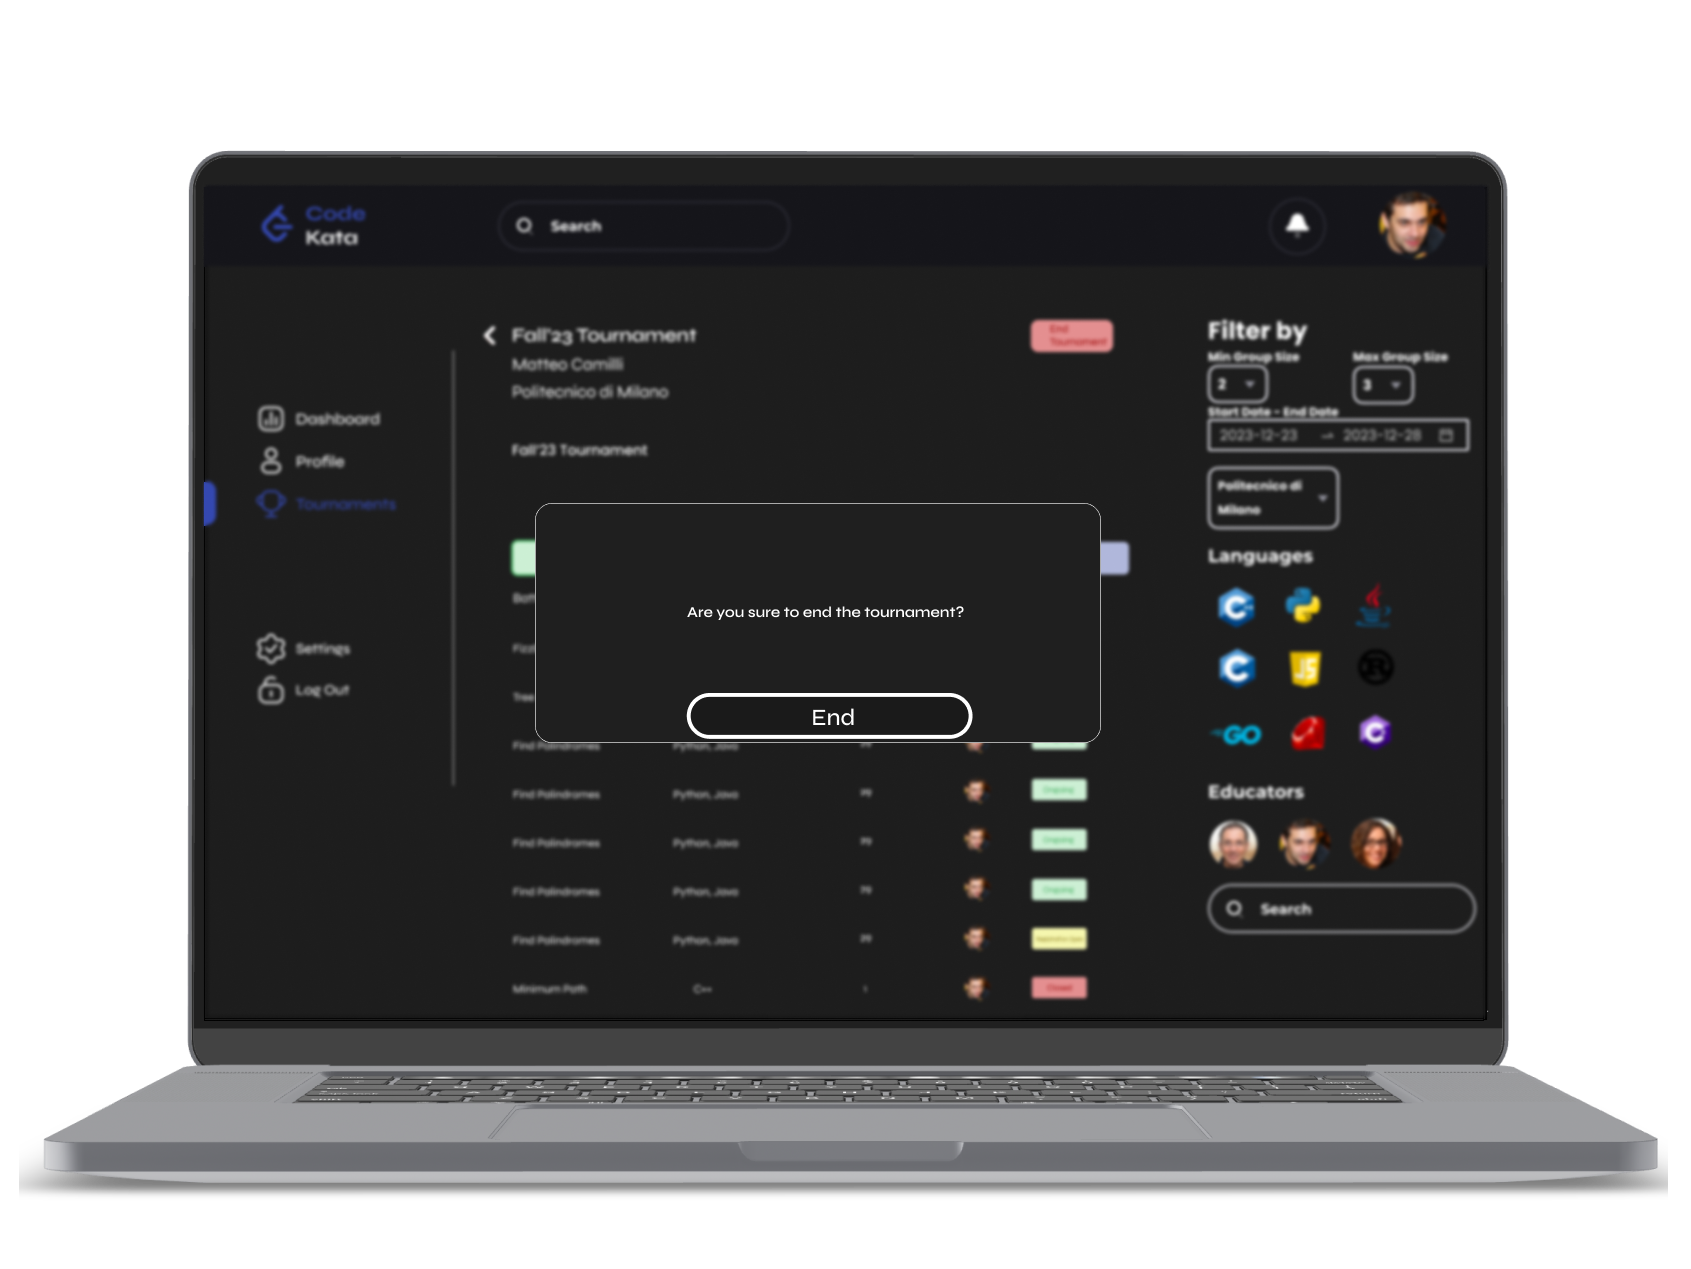
\includegraphics[scale=0.13]{Images/ui-ux/educator_end_tournament_1.png}
        (p) $UI_{16}$  Educator Ends Tournament
\end{center}

\begin{itemize}
    \item \textbf{$UI_{1}$:} This is a mockup for registration of students and educators. $RW_{1}$ is the related runtime diagram for this mockup.
    \item \textbf{$UI_{2}$:} This is mockup for student and educator login. $RW_{2}$ is the related runtime diagram for this mockup.
    \item \textbf{$UI_{3}$:} These are the screens of the student when it enters the application. This screens is created by fetching tournament with different filters.
    \item \textbf{$UI_{4}$:} These are screens of tournaments from students' perspective. Also these screens are related to  $RW_{3}$. Student can easily navigate among different tournaments.
    \item \textbf{$UI_{5}$:} These are screens of a single tournament from users' perspective. Also these screens are related to  $RW_{3}$. User can easily navigate among battles and leaderboard.
    \item \textbf{$UI_{6}$:} In this screen student register for battle by choosing "register as team" option. The following user interfaces $UI_{7}$ also explain the next steps from this design. Related to $RW_{10}$
    \item \textbf{$UI_{7}$:} This screens shows possible states of a battle screen for a student. Also related to $RW_{4}$ and and $RW_{10}$.
    \item \textbf{$UI_{8}$:} Profile and Setting screens of a student. Related to $RW_{5}$
    \item \textbf{$UI_{9}$:} These are the screens of the educator when it enters the application. This screens is created by fetching tournament with different filters.
    \item \textbf{$UI_{10}$:} These are screens of tournaments from educators' perspective. Also these screens are related to  $RW_{3}$. Educators can easily navigate among different tournaments.
    \item \textbf{$UI_{11}$:} These screens demonstrate the pages for tournament creation. As you can see another educators can be invited. Related to $RW_{6}$ and $RW_{11}$
    \item \textbf{$UI_{12}$:} These screens demonstrate the pages for battle creation. Related to $RW_{6}$ and $RW_{12}$
    \item \textbf{$UI_{13}$:} These screens demonstrate the pages for viewing a battle.  Related to $RW_{4}$
    \item \textbf{$UI_{14}$:} These screen shows how educators can see a submission made by students. Also it demonstrates the manual scoring.
    Related to $RW_{13}$, $RW_{14}$ and $RW_{15}$
    \item \textbf{$UI_{15}$:} Profile and Setting screens of a educator. Related to $RW_{5}$
    \item \textbf{$UI_{16}$:} Educator ends tournament.
\end{itemize}

\newpage


%------------------------------------------------------------------------------------------------------------------------------------------------
\clearpage
{\color{Blue}{\section{Requirements Traceability}}}
\label{sect:reqs}
In this section, we are going to illustrate the mapping of the components introduced in this document on the functional requirements introduced in the RASD. Some closely related requirements are explained together in the tables below.

\begin{table}[h!]
  \centering
  \begin{tabular}{lp{12cm}}
    \hline
    \textbf{R1} & The system shall allow unregistered users to register by providing a unique email, a password, a name, a surname, and institution information. \\
    \hline
    \hline
    \textbf{Authentication Manager} & Gets the client request, and directs it to User Repository. \\
    \textbf{User Repository} &  Creates the user.\\
    \textbf{DBMS} & Saves the user. \\
    \textbf{Notification Manager} &  Triggers Email Manager.\\
    \textbf{Email Manager} &  Sends verification email.\\
    \hline
  \end{tabular}
  \captionof{table}{Mapping on $R_{1}$}
\end{table}

\begin{table}[h!]
  \centering
  \begin{tabular}{lp{12cm}}
    \hline
    \textbf{R2} & The system shall allow users who received a verification email to verify their emails. \\
    \hline
    \hline
    \textbf{Authentication Manager} & Gets the client request, and directs it to User Repository. \\
    \textbf{User Repository} &  Verifies the user.\\
    \textbf{DBMS} & Updates the user. \\
    \hline
  \end{tabular}
  \captionof{table}{Mapping on $R_{2}$}
\end{table}

\begin{table}[h!]
  \centering
  \begin{tabular}{lp{12cm}}
    \hline
    \textbf{R3} & The system shall allow registered users to log in by providing an email, and a password. \\
    \hline
    \hline
    \textbf{Authentication Manager} & Gets the client request, and directs it to User Repository. \\
    \textbf{User Repository} &  Validates the user credentials.\\
    \textbf{DBMS} & Returns user info. \\
    \hline
  \end{tabular}
  \captionof{table}{Mapping on $R_{3}$}
\end{table}

\begin{table}[h!]
  \centering
  \begin{tabular}{lp{12cm}}
    \hline
    \textbf{R4} & The system shall allow authenticated users to view all tournaments. \\
    \hline
    \hline
    \textbf{Tournament Manager} & Gets the client request, and directs it to Tournament Repository. \\
    \textbf{Tournament Repository} &  Gets all tournaments.\\
    \textbf{DBMS} & Returns all tournaments. \\
    \hline
  \end{tabular}
  \captionof{table}{Mapping on $R_{4}$}
\end{table}

\begin{table}[h!]
  \centering
  \begin{tabular}{lp{12cm}}
    \hline
    \textbf{R5} & The system shall allow authenticated users to filter the tournaments by the registration status and availability.  \\
    \hline
    \hline
    \textbf{Tournament Manager} & Gets the client request, and directs it to Tournament Repository. \\
    \textbf{Tournament Repository} &  Gets filtered tournaments using a query.\\
    \textbf{DBMS} & Returns queried tournaments. \\
    \hline
  \end{tabular}
  \captionof{table}{Mapping on $R_{5}$}
\end{table}

\begin{table}[h!]
  \centering
  \begin{tabular}{lp{12cm}}
    \hline
    \textbf{R6} & The system shall allow authenticated users to sort the tournaments by number of participants and number of battles in it. \\
    \hline
    \hline
    \textbf{Tournament Manager} & Gets the client request, and directs it to Tournament Repository. \\
    \textbf{Tournament Repository} &  Gets sorted tournaments using a query.\\
    \textbf{DBMS} & Returns queried tournaments. \\
    \hline
  \end{tabular}
  \captionof{table}{Mapping on $R_{6}$}
\end{table}

\begin{table}[h!]
  \centering
  \begin{tabular}{lp{12cm}}
    \hline
    \textbf{R7} & The system shall allow authenticated users to view a specific tournament. \\
    \hline
    \hline
    \textbf{Tournament Manager} & Gets the client request, and directs it to Tournament Repository. \\
    \textbf{Tournament Repository} &  Gets the tournament by its id using a query.\\
    \textbf{DBMS} & Returns queried tournament. \\
    \hline
  \end{tabular}
  \captionof{table}{Mapping on $R_{7}$}
\end{table}

\begin{table}[h!]
  \centering
  \begin{tabular}{lp{12cm}}
    \hline
    \textbf{R8} & The system shall allow authenticated users to view the leaderboard of the tournament. \\
    \hline
    \hline
    \textbf{Tournament Manager} & Gets the client request, and directs it to Tournament Repository. \\
    \textbf{Tournament Repository} &  Gets the tournament scores of subscribed users and then sorts them.\\
    \textbf{DBMS} & Returns tournament scores. \\
    \hline
  \end{tabular}
  \captionof{table}{Mapping on $R_{8}$}
\end{table}

\begin{table}[h!]
  \centering
  \begin{tabular}{lp{12cm}}
    \hline
    \textbf{R9} & The system shall allow authenticated users to view all battles in a tournament. \\
    \hline
    \hline
    \textbf{Tournament Manager} & Gets the client request, and directs it to Tournament Repository. \\
    \textbf{Tournament Repository} &  Gets the list of battles of the tournament.\\
    \textbf{DBMS} & Returns the list of battles. \\
    \hline
  \end{tabular}
  \captionof{table}{Mapping on $R_{9}$}
\end{table}

\begin{table}[h!]
  \centering
  \begin{tabular}{lp{12cm}}
    \hline
    \textbf{R10} & The system shall allow authenticated users to filter the battles by group size, start date - end date, registration status, institution of the battle creator, allowed programming languages, and the battle creator. \\
    \hline
    \hline
    \textbf{Battle Manager} & Gets the client request, and directs it to Battle Repository. \\
    \textbf{Battle Repository} &  Gets filtered battles using a query.\\
    \textbf{DBMS} & Returns queried battles. \\
    \hline
  \end{tabular}
  \captionof{table}{Mapping on $R_{10}$}
\end{table}

\begin{table}[h!]
  \centering
  \begin{tabular}{lp{12cm}}
    \hline
    \textbf{R11} & The system shall allow authenticated users to search battles by text search. \\
    \hline
    \hline
    \textbf{Battle Manager} & Gets the client request, and directs it to Battle Repository. \\
    \textbf{Battle Repository} &  Gets searched battles using a query.\\
    \textbf{DBMS} & Returns queried battles. \\
    \hline
  \end{tabular}
  \captionof{table}{Mapping on $R_{11}$}
\end{table}

\begin{table}[h!]
  \centering
  \begin{tabular}{lp{12cm}}
    \hline
    \textbf{R12} & The system shall allow authenticated users to view a specific battle and its instructions. \\
    \hline
    \hline
    \textbf{Battle Manager} & Gets the client request, and directs it to Battle Repository. \\
    \textbf{Battle Repository} &   Gets the battle by its id using a query.\\
    \textbf{DBMS} & Returns queried battle. \\
    \hline
  \end{tabular}
  \captionof{table}{Mapping on $R_{12}$}
\end{table}

\begin{table}[h!]
  \centering
  \begin{tabular}{lp{12cm}}
    \hline
    \textbf{R13} & The system shall allow authenticated users to view the rankings of the battle. \\
    \hline
    \hline
    \textbf{Battle Manager} & Gets the client request, and directs it to Battle Repository. \\
    \textbf{Battle Repository} & Gets the battle scores of participating teams and then sorts them.\\
    \textbf{DBMS} & Returns battle scores. \\
    \hline
  \end{tabular}
  \captionof{table}{Mapping on $R_{13}$}
\end{table}

\begin{table}[h!]
  \centering
  \begin{tabular}{lp{12cm}}
    \hline
    \textbf{R14} & The system shall allow authenticated users to search tournaments with text search by educators, by titles, or by institutions.\\
    \hline
    \hline
    \textbf{Tournament Manager} & Gets the client request, and directs it to Tournament Repository. \\
    \textbf{Tournament Repository} & Gets searched tournaments using a query.\\
    \textbf{DBMS} & Returns queried tournaments. \\
    \hline
  \end{tabular}
  \captionof{table}{Mapping on $R_{14}$}
\end{table}

\begin{table}[h!]
  \centering
  \begin{tabular}{lp{12cm}}
    \hline
    \textbf{R15} & The system shall allow authenticated users to manage their profiles.
  \begin{enumerate}[(a)]
      \item The system shall allow authenticated users to view their profiles.
      
  \item The system shall allow authenticated users to delete their profiles unless they do not have an ongoing tournament created by themselves.

    \item The system shall allow authenticated users to view their settings.
  \item The system shall allow authenticated users to edit their settings by name, surname, password, and institution information.
  \item The system shall oblige authenticated users to enter their old password during settings editing.
  
      
  \end{enumerate}
\\
    \hline
    \hline
    \textbf{Profile Manager} & Gets the client request, and directs it to User Repository. \\
    \textbf{User Repository} & \begin{enumerate}[(a)]
      \item Gets the user profile.
      
  \item Deletes the user.
    \item Gets the user settings.
  \item Edits the user settings.
  \item Edits the user settings.
  
      
  \end{enumerate}
    
    \\
    \textbf{DBMS} & \begin{enumerate}[(a)]
      \item Returns user profile.
      
  \item Removes user.

    \item Returns user settings.
  \item Updates user settings.
\item Updates user settings.
  
      
  \end{enumerate}
    
    
    
    \\
    \hline
  \end{tabular}
  \captionof{table}{Mapping on $R_{15}$}
\end{table}



\begin{table}[h!]
  \centering
  \begin{tabular}{lp{12cm}}
    \hline
    \textbf{R16} & The system shall allow educators to create tournaments by providing a title, a description, and a registration 
    deadline. \\
    \textbf{R34} & The system shall trigger the email service to send a notification email for a newly created tournament for all registered users.\\
    \hline
    \hline
    \textbf{Tournament Manager} & Gets the client request, and directs it to Tournament Repository. \\
    \textbf{Tournament Repository} & Creates the tournament.\\
    \textbf{DBMS} & Saves the tournament. \\
    \textbf{Notification Manager} &  Triggers Email Manager.\\
    \textbf{Email Manager} &  Sends notification email to all users.\\
    \hline
  \end{tabular}
  \captionof{table}{Mapping on $R_{16}$ and $R_{34}$}
\end{table}


\begin{table}[h!]
  \centering
  \begin{tabular}{lp{12cm}}
    \hline
    \textbf{R17} & The system shall allow educators to invite other educators to their tournaments during tournament creation. \\
    \textbf{R37} & The system shall trigger the email service to send an invitation notification for the tournament to the invitee educators.\\
    \hline
    \hline
    \textbf{Tournament Manager} & Gets the client request, and directs it to Tournament Repository. \\
    \textbf{Tournament Repository} & Creates the tournament.\\
    \textbf{DBMS} & Saves the tournament. \\
    \textbf{Notification Manager} &  Triggers In-App Notification Manager.\\
    \textbf{In-App Notification Manager} &  Sends invitation notification to invitee educators.\\
    \hline
  \end{tabular}
  \captionof{table}{Mapping on $R_{17}$ and $R_{37}$}
\end{table}

\begin{table}[h!]
  \centering
  \begin{tabular}{lp{12cm}}
    \hline
    \textbf{R18} & The system shall allow educators to edit the tournaments that they have created by providing a title, a description, and a registration deadline unless the registration deadline has not passed. \\
    \hline
    \hline
    \textbf{Tournament Manager} & Gets the client request, and directs it to Tournament Repository. \\
    \textbf{Tournament Repository} & Edits the tournament.\\
    \textbf{DBMS} & Updates the tournament. \\
    \hline
  \end{tabular}
  \captionof{table}{Mapping on $R_{18}$}
\end{table}

\begin{table}[h!]
  \centering
  \begin{tabular}{lp{12cm}}
    \hline
    \textbf{R19} & The system shall allow educators to end the tournaments that they have created. \\
    \hline
    \hline
    \textbf{Tournament Manager} & Gets the client request, and directs it to Tournament Repository. \\
    \textbf{Tournament Repository} & Ends the tournament.\\
    \textbf{DBMS} & Updates the tournament. \\
    \hline
  \end{tabular}
  \captionof{table}{Mapping on $R_{19}$}
\end{table}

\begin{table}[h!]
  \centering
  \begin{tabular}{lp{12cm}}
    \hline
    \textbf{R20} & The system shall allow educators to accept or reject the tournament invitation to create battles coming from other educators for a tournament. \\
    \hline
    \hline
    \textbf{Tournament Manager} & Gets the client request, and directs it to Tournament Repository. \\
    \textbf{Tournament Repository} & Adds the educator to the tournament contributors list.\\
    \textbf{DBMS} & Updates the tournament. \\
    \hline
  \end{tabular}
  \captionof{table}{Mapping on $R_{20}$}
\end{table}


\begin{table}[h!]
  \centering
  \begin{tabular}{lp{12cm}}
    \hline
    \textbf{R21} & The system shall allow educators to create battles by providing a title, a description, a registration deadline, a submission deadline, the allowed languages, test cases, build scripts, minimum \& maximum group size, and the scoring criteria. \\
    \hline
    \hline
    \textbf{Battle Manager} & Gets the client request, and directs it to Battle Repository. \\
    \textbf{Battle Repository} & Creates the battle.\\
    \textbf{DBMS} & Saves the battle. \\
    \textbf{Notification Manager} &  Triggers Email Manager.\\
    \textbf{Email Manager} &  Sends notification email to users that subscribe to the battle's tournament.\\
    \hline
  \end{tabular}
  \captionof{table}{Mapping on $R_{21}$}
\end{table}


\begin{table}[h!]
  \centering
  \begin{tabular}{lp{12cm}}
    \hline
    \textbf{R22} & The system shall oblige educators to upload test case file and build script for every allowed language in battle. \\
    \hline
    \hline
    \textbf{Battle Manager} & Gets the client request, and uploads the battle files. \\
    \textbf{File Manager} & Stores the battle files. \\
    \hline
  \end{tabular}
  \captionof{table}{Mapping on $R_{22}$}
\end{table}

\begin{table}[h!]
  \centering
  \begin{tabular}{lp{12cm}}
    \hline
    \textbf{R23} & The system shall allow educators to manually evaluate the submissions giving extra point between 0 and 10 after the submission deadline has passed. \\
    \hline
    \hline
    \textbf{Battle Manager} & Gets the client request, and directs it to Submission Manager. \\
    \textbf{Submission Manager} & Utilises Scoring Manager, and gives the score to the Submission Repository.\\
    \textbf{Scoring Manager} & Enables educator to evaluate. \\
     \textbf{Submission Repository} & Gives point to the submission.\\
     \textbf{DBMS} & Updates the submission. \\
    \hline
  \end{tabular}
  \captionof{table}{Mapping on $R_{23}$}
\end{table}

\begin{table}[h!]
  \centering
  \begin{tabular}{lp{12cm}}
    \hline
    \textbf{R24} & The system shall allow educators to edit the battles that they have created. \\
    \hline
    \hline
     \textbf{Battle Manager} & Gets the client request, and directs it to Battle Repository. \\
    \textbf{Battle Repository} & Edits the battle.\\
    \textbf{DBMS} & Updates the battle. \\
    \hline
  \end{tabular}
  \captionof{table}{Mapping on $R_{24}$}
\end{table}

\begin{table}[h!]
  \centering
  \begin{tabular}{lp{12cm}}
    \hline
    \textbf{R25} &  The system shall allow students to register for tournaments. \\
    \hline
    \hline
     \textbf{Tournament Manager} & Gets the client request, and directs it to Tournament Repository. \\
    \textbf{Tournament Repository} & Adds the student to the tournament subscribers.\\
    \textbf{DBMS} & Updates the tournament. \\
    \hline
  \end{tabular}
  \captionof{table}{Mapping on $R_{25}$}
\end{table}


\begin{table}[h!]
  \centering
  \begin{tabular}{lp{12cm}}
    \hline
    \textbf{R26} &  The system shall allow students to register for battles in which the tournaments that they have registered for.\\
    \textbf{R27} &  The system shall allow students to register for battles individually.\\
    \textbf{R28} &  The system shall allow students to register for battles by a team having a team name.\\
    \hline
    \hline
    \textbf{Battle Manager} & Gets the client request, and triggers Team Manager. With the response coming from the Team Manager, it utilises Battle Repository.\\
    \textbf{Team Manager} & Creates a team. (Regardless of the number of students on the team, it is created. Individual students will be considered as a team of one in the project.)\\
    \textbf{Team Repository} & Creates the team.\\
    \textbf{Battle Repository} & Adds the team to the battle participants.\\
    \textbf{DBMS} & Saves the team, and updates the battle. \\
    \hline
  \end{tabular}
  \captionof{table}{Mapping on $R_{26}$, $R_{27}$, $R_{28}$}
\end{table}

\begin{table}[h!]
  \centering
  \begin{tabular}{lp{12cm}}
    \hline
    \textbf{R29} &  The system shall allow students to invite other students to their team during battle registration. \\
    \textbf{R35} &  The system shall trigger the email service to send an invitation notification for the battle to the invitee students. \\
    \hline
    \hline
    \textbf{Battle Manager} & Gets the client request, and directs it to Team Manager. \\
    \textbf{Team Manager} & Notifies invitee students.\\
    \textbf{Notification Manager} &  Triggers In-App Notification Manager.\\
    \textbf{In-App Notification Manager} &  Sends invitation notification to invitee students.\\
    \hline
  \end{tabular}
  \captionof{table}{Mapping on $R_{29}$}
\end{table}

\begin{table}[h!]
  \centering
  \begin{tabular}{lp{12cm}}
    \hline
    \textbf{R30} &  The system shall allow students to accept or reject the team invitation coming from other students for a battle. \\
    \hline
    \hline
    \textbf{Battle Manager} & Gets the client request, and directs it to Team Manager. \\
    \textbf{Team Manager} & Utilises Team Repository.\\
    \textbf{Team Repository} & Adds the student to the team members.\\
    \textbf{DBMS} & Updates the team. \\
    \hline
  \end{tabular}
  \captionof{table}{Mapping on $R_{30}$}
\end{table}


\begin{table}[h!]
  \centering
  \begin{tabular}{lp{12cm}}
    \hline
    \textbf{R31} &  The system shall allow students to finalize their team registration or decline it. \\
    \hline
    \hline
    \textbf{Battle Manager} & Gets the client request, and directs it to Team Manager. \\
    \textbf{Team Manager} & Utilises Team Repository.\\
    \textbf{Team Repository} & Finalises or declines the team.\\
    \textbf{DBMS} & Updates or removes the team. \\
    \hline
  \end{tabular}
  \captionof{table}{Mapping on $R_{31}$}
\end{table}


\begin{table}[h!]
  \centering
  \begin{tabular}{lp{12cm}}
    \hline
    \textbf{R32} &  The system shall create a repository for a battle after the registration deadline for that battle has passed. \\
    \textbf{R36} &  The system shall trigger the email service to send a notification email including the link to the battle repository to the students registered for it.\\
    \hline
    \hline
    \textbf{Battle Manager} & Initialises repo creation for a battle. \\
    \textbf{GitHub Manager} & Creates repository, return the URL to the Battle Manager.\\
    \textbf{Battle Repository} & Adds repository URL to the battle.\\
    \textbf{DBMS} & Updates the battle. \\
    \textbf{Notification Manager} &  Triggers Email Manager.\\
    \textbf{Email Manager} &  Sends notification email to the users that participate in the battle.\\
    
    \hline
  \end{tabular}
  \captionof{table}{Mapping on $R_{32}$ and $R_{36}$}
\end{table}


\begin{table}[h!]
  \centering
  \begin{tabular}{lp{12cm}}
    \hline
    \textbf{R33} &  The system shall pull the repository of a team following a trigger from GitHub Actions. \\
    \hline
    \hline
    \textbf{Submission Manager} & Triggered by GitHub Actions, utilises GitHub Manager and File Manager. \\
    \textbf{GitHub Manager} & Pulls the repository.\\
    \textbf{File Manager} & Stores the files retrieved from repository.\\
    \hline
  \end{tabular}
  \captionof{table}{Mapping on $R_{33}$}
\end{table}





\begin{table}[h!]
  \centering
  \begin{tabular}{lp{12cm}}
    \hline
    \textbf{R38} & The system shall automatically evaluate submissions by scoring criteria.
     \begin{enumerate}[(a)]
         \item The system shall score the submission with respect to test cases, and test case weight.
         \item The system shall score the submission with respect to timeliness, and timeliness weight.
         \item The system shall score the submission with respect to quality aspects, and quality aspect weight.
     \end{enumerate}
\\
 \textbf{R39} & The system shall utilise a Static Analysis Tool to calculate the score in terms of quality aspects.\\
 \textbf{R40} & The system shall create a sandbox environment for each team for the submissions in order to run the codes.\\
    \hline
    \hline
    \textbf{Submission Manager} & Gets submission files and send them to evaluation. \\
    \textbf{File Manager} & Retrieves previously stored files from File Storage.\\
    \textbf{Scoring Manager} &  Calculates test case scores and timeliness. Gets help from Static Analysis Manager to calculate static analysis score.\\
    \textbf{Sandbox Manager} & Creates sandbox environment, runs the code, returns the output. Kills the environment after usage.\\
    \textbf{Static Analysis Manager} & Utilises Static Analyser in order to calculate Static Analysis Score. \\
    \textbf{Static Analyser Subsystem} & Calculates static analysis score.\\
    \hline
  \end{tabular}
  \captionof{table}{Mapping on $R_{38}$, $R_{39}$, $R_{40}$}
\end{table}

\begin{table}[h!]
  \centering
  \begin{tabular}{lp{12cm}}
    \hline
    \textbf{R41} &  The system shall automatically update the battle score of a team after the evaluation of the submission. \\
    \hline
    \hline
    \textbf{Submission Manager} & Delivers the evaluation result to the Submission Repository. \\
    \textbf{Submission Repository} & Gives score to the submission.\\
    \textbf{DBMS} & Updates the submission.\\
    \hline
  \end{tabular}
  \captionof{table}{Mapping on $R_{41}$}
\end{table}


\begin{table}[h!]
  \centering
  \begin{tabular}{lp{12cm}}
    \hline
\textbf{R42} & The system shall automatically update the battle rankings when a score is updated. \\
    \hline
    \hline
    \textbf{Battle Manager} &  Retrieves scores to display battle rankings.\\
    \textbf{Battle Repository} & Gets the battle scores of participating teams and then sorts them.\\
    \textbf{DBMS} & Returns battle scores. \\
    \hline
  \end{tabular}
  \captionof{table}{Mapping on $R_{42}$}
\end{table}


\begin{table}[h!]
  \centering
  \begin{tabular}{lp{12cm}}
    \hline
    \textbf{R43} & The system shall automatically update the tournament leaderboard at the end of each battle. \\
    \hline
    \hline
    \textbf{Tournament Manager} & Retrieves the tournament scores to display the leaderboard. \\
    \textbf{Tournament Repository} &  Gets the tournament scores of subscribed users and then sorts them.\\
    \textbf{DBMS} & Returns tournament scores. \\
    \hline
  \end{tabular}
  \captionof{table}{Mapping on $R_{43}$}
\end{table}

%------------------------------------------------------------------------------------------------------------------------------------------------
%------------------------------------------------------------------------------------------------------------------------------------------------
\clearpage
{\color{Blue}{\section{Implementation, Integration, and Test Plan}}}
\label{sect:imp}
In this section, we briefly explained the planned implementation, integration and testing of system components. 

\subsection{Implementation}
\indent The system is structured around three primary layers: client, application, and data. These will be concurrently developed and later integrated. By doing so, each layer can be tested individually, and after integration, comprehensive system-wide testing can be conducted. We will employ a hybrid strategy, combining bottom-up and thread methodologies, to leverage the advantages of both.
\\
\indent The thread approach aids in creating interim deliverables for stakeholder evaluation, proving extremely beneficial for system validation. Concurrently, the bottom-up strategy facilitates incremental integration, enhancing bug detection by allowing for the testing of subsystems as they progressively evolve through the addition of new modules.
\\
\indent The thread strategy involves pinpointing the system's functionalities and the specific segments of the components (termed as sub-components for practical purposes, though they may not align precisely with design sub-components) that are responsible for these functionalities. Since multiple sub-components collaboratively contribute to a single function, it's crucial to establish a sequence for their implementation, for which the bottom-up approach is particularly useful.
\\
\indent This mixed strategy enables the allocation of different feature implementations to independent development teams working in parallel. However, it's essential to identify any common components beforehand to prevent duplication of efforts in creating the same component or sub-component more than once. This approach not only streamlines the development process but also ensures a more efficient and organized integration of the various system parts.

\subsubsection{Client Application}
Static parts of Client Web Application ,in other words Frontend, can be implemented without server side implementation. Mockups and UI-UX design can be used for this development. However, dynamic actions rely on REST API to communicate server-side responsible for business logic. So, using documentation, unit test mocking REST API can be used to implement Frontend code.
\subsubsection{Application Layer}
Application Layer, in other words Backend, is responsible for the business logic in server side. We can separate some parts of the Application Layer to be developed in parallel.
The components to be incorporated into the system are derived directly from the system's requirements. The developers can be work separately on these components and integrate and test at the end of their development the components to evaluate the dependency and the interactions between them. The entire business logic can be tested separately from the client logic, which accelerates the development process. Below is a concise summary of the system's components with priorities.
\begin{tabularx}{0.8\textwidth} { 
  | >{\raggedright\arraybackslash}X 
  | >{\centering\arraybackslash}X 
  | >{\raggedleft\arraybackslash}X | }
 \hline
\textbf{Component} & \textbf{Importance} &  \textbf{Complexity} \\
 \hline
 Authentication Manager  & High  & Low  \\
  \hline
 Profile Manager  & Medium  & Low  \\
\hline
 Tournament Manager  & Medium  & High  \\
\hline
 Battle Manager  & Medium  & High  \\
\hline
 Team Manager  & Medium  & Low  \\
\hline
 Notification Subsystem Components  & Low  & Medium  \\
\hline
 Repository Components  & High  & Medium  \\
\hline
 Submission Manager  & Medium  & Medium  \\
\hline
 Github Manager  & Low  & Low  \\
\hline
 Scoring Manager  & High  & Medium  \\
\hline
 File Manager  & Medium  & Low  \\
\hline
 Static Analysis Subsystem Components  & Medium  & High  \\
\hline
\end{tabularx}

So, briefly, we have to consider the importance and complexity of a component before starting to implement the component. This kind of analysis enables us to estimate time and work cost spent for a certain part of application.
\\

\subsubsection{Implementation Plan}
\begin{enumerate}
    \item \textbf{Repository Components:} For the application, data access layer has a great importance because all other components mainly rely on data access at some point. Database interaction is crucial because of the CRUD operations. So Tournament, Battle, User, Team and Submission Repository components are implemented firstly in parallel because there is no dependency between them.
    \item \textbf{Notification Manager:} Even though a notification system is not a crucial part of the system, it's methods widely used by lots of components, so implementing it at early stages can be very helpful to see its usage among other components when implementing them. EmailManager and InAppNotificationManager are another required components for the Notification Component and they are considered within Notification Manager Component.
    \item \textbf{Authentication Manager:} This component offers 2 interfaces which is related to users' authentication. \textbf{Registration, login and logout} functionalities are very fundamental to operate all business logic. Also it provides a session manager interface which is used by other components in which it is important to know who the user is, what type it is and what permissions it has.
    \item \textbf{Tournament Manager:} Implementation of this component  can be at the end if we follow just bottom-up approach. However, one of our goals is to create intermediate products and this component, even if it is a complex component, can helps us to create such an intermediate product. It has also no dependency other than Tournament Repository, Notification Manager and Authentication Manager.
    \item \textbf{File Manager:} This component mainly responsible to communicate with File Storage Service. It encapsulate the operations such as fetch,read or write file from or to the file system on the cloud. It provides an interface to manage files so it is needed by other components.
    \item \textbf{Profile Manager:} Unlikely to Tournament, this component has really low complexity without no real dependency other than repositories. By implementing Profile Manager at early stages, we can achieve a intermediate product with less effort and no dependency is needed.
    \item \textbf{Scoring Manager:} Again this is another components which is responsible to communicate to an external service. Also it provides an iterface to calculate score of a submission. This component also has high priority with its required components such as Sandbox Manager and Static Analysis Manager.
    \item \textbf{Github Manager:} Even though Github Manager is not fundamental as some main components such as Submission Manager and Battle Manager, implementing it early comes with advantages. It provides interfaces to these components. Also there can be another components using some logic related to Github. 
    \item \textbf{Submission Manager:} This component is one of the main components in the application which provides Submission related methods. It is very critic to use because it also provides an endpoint to be triggered by Github. 
    \item \textbf{Team Manager}: It provides interface related to team operations. Needed from Battle Manager.
    \item \textbf{Battle Manager:} These components provides the endpoints about Battles and operates the logic related to Battles. It uses various interfaces from various components so it is good to implement this component at the last stages.
    \item \textbf{Static Analysis Subsystem:} These components are part of the Static Analysis Subsystem. Scanner, Analysis Server and Database are implemented at the the end because it just communicates with the static analysis scoring and can be easily mocked. However, without integration this part can be implemented in parallel.
\end{enumerate}

\newpage
\subsection{Integration}
\indent The section describes the integration plan of the different components and subcomponents of the CodeKataBattle. The provided graphs illustrate the interdependencies between various components and subcomponents. Before any subcomponent is combined with others to create a larger component, it must undergo unit testing. Following this integration, the complete component is then subjected to further testing.
\\
\indent Before proceeding with the integration testing of a component, it is crucial to satisfy two key conditions, each with its distinct benefits. The first condition is that the component's interface must encompass all the functionalities detailed in the component interface diagram. This ensures that the component adheres to the predefined design specifications, which is vital for maintaining consistency and predictability in the system’s overall behavior. Adhering to these specifications also facilitates easier integration with other components, as each piece is designed to fit seamlessly within the broader system architecture.
\\
\indent The second prerequisite is that the component must successfully clear all unit tests. Unit testing plays a critical role in verifying that each individual part of the component functions as intended in isolation. This process helps in identifying and rectifying any bugs or issues at an early stage, significantly reducing the risk of defects in the later stages of development. Successful unit testing guarantees a higher level of reliability and stability in the component, which in turn contributes to the robustness of the final integrated system. By ensuring that each component is thoroughly tested and fully functional before integration, the overall quality and performance of the system are enhanced, leading to a more efficient, reliable, and effective product.
\\
\indent As you can see the diagrams below, Driver is used as unit test to mock the not-finished components. This part is crucial during the integration test written here should be passed. 

\newpage
\indent First integration to be handled is integrating \textbf{Repository Components} to DBMS in order to sustain a working data access layer. To enable other components to handle data this integration is very crucial. This is a prelimanary integration with DBMS. Unit Testing is used to mock the  other components being under development. This Driver is mainly responsible to mock repository calls from the components using them. Moreover, it checks the validity of the results.

\begin{figure}[H]
    \centering
    \includegraphics[width=\linewidth]{Images/integration/integration_1.drawio.png}
    \caption{Integration of Repository Components}
\end{figure}

\newpage
\indent Notification subsystem is integrated then to be used by other following components. It is very crucial here, after implementing EmailManager and InAppNotificationManager according to the external APIs, NotificationManager is implemented because there exists a dependency between NotificationManager and other two components. Testing is done as explained above with mocking usage of notification according to INotificationManager interface documentation. 

\begin{figure}[H]
    \centering
    \includegraphics[width=\linewidth]{Images/integration/integration_2.drawio.png}
    \caption{Integration of Notification Subsystem}
\end{figure}

\newpage
\indent Authentication Manager is the component responsible for authentication operations. Its integration is done after implementing user repository and notification subsystem. In this stage of development, we are able to implement functions mocked for User Repository and Notification subsystem. Naturally, Unit tests must be passed before and after integration of Authentication Manager Component to these components. At this point, we also have some endpoints to Client Application after integration, so we can do Register, Login, Logout operations end-to-end. Application Server is developing independently, so we will use and test endpoints with the help of some tools such as Postman. At this time, it would be very helpful to start a Postman collection to document the endpoints.

\begin{figure}[H]
    \centering
    \includegraphics[width=\linewidth]{Images/integration/integration_3.drawio.png}
    \caption{Integration of Authentication Manager Component}
\end{figure}

\newpage
\indent Tournament Manager helps us to create an intermediate product because it has very few dependencies. At this stage, we integrated it to developed parts of application. Unit tests must be passed before and after integration. There will be some operations requires to send notification via email and in-app notification. Especially, for Notification Subsystem, implementing this functions must be aligned with unit tests. 

\begin{figure}[H]
    \centering
    \includegraphics[width=\linewidth]{Images/integration/integration_4.drawio.png}
    \caption{Integration of Tournament Manager Component}
\end{figure}

\newpage
\indent File Manager can be developed and integrated to File Storage Service independently. This is also can be done in parallel to other components above. 

\begin{figure}[H]
    \centering
    \includegraphics[width=\linewidth]{Images/integration/integration_5.drawio.png}
    \caption{Integration of File Manager Component}
\end{figure}

\newpage
\indent Profile Manager is another component to help to create intermediate product with the components Authentication Manager and Tournament Manager. It is integrated to User Repository and File System Manager for the profile specific operations. Also similar to Tournament Manager it uses session information from Authentication Manager and dependent on it. File Manager is integrated to all system via Profile Manager at this stage.

\begin{figure}[H]
    \centering
    \includegraphics[width=\linewidth]{Images/integration/integration_6.drawio.png}
    \caption{Integration of Profile Manager Component}
\end{figure}

\newpage
\indent Scoring Manager and Github Manager can be implemented and integrated in parallel. For Scoring Manager, there are two other components which are responsible to Sandbox Manager and Static Analysis Manager. Firstly, Static Analysis Manager is integrated to Static Analysis Subsystem, then it is integrated to Scoring Manager with Sandbox Manager. For now, we mock the Static Analysis Subsytem. Also Github Manager is integrated to Github with necessary documentation provided by Github.

\begin{figure}[H]
    \centering
    \includegraphics[width=\linewidth]{Images/integration/integration_7.drawio.png}
    \caption{Integration of Scoring and Github Manager}
\end{figure}

\newpage
\indent Submission Manager has a dependency over Scoring Manager, Github Manager and File Manager. Its implementation and integration will be held after these components. Also, usage of these components' provided interfaces from Submission Manager should be aligned with unit test written before for these components. Submission Manager is still separated from the application because mainly Battle Manager uses the interface provided by Submission Manager.

\begin{figure}[H]
    \centering
    \includegraphics[width=\linewidth]{Images/integration/integration_8.drawio.png}
    \caption{Integration of Submission Manager}
\end{figure}

\newpage
\indent At the end Battle Manager, which uses repository components, scoring and Github related actions via Submission Manager and session methods, is implemented and integrated. Of course, Team Manager is firstly implemented and integrated to Battle Manager with the help of  some unit test. Then Battle Manager integrated to Submission Manager, Authentication Manager, Repository Components, File Manager and Notification Manager. As you can see, it needs lots of components to be implemented to  operate and be integrated to application. 

\begin{figure}[H]
    \centering
    \includegraphics[width=\linewidth]{Images/integration/integration_9.drawio.png}
    \caption{Integration of Battle and Team Manager}
\end{figure}

\newpage
\indent Until now, we have mocked the Static Analysis Subsystem. It is implemented and integrated at the end. Its internal implementation is bottom-up. We firstly create db, then server. Our scanner is responsible for outer communication and scanning the code to be analyzed on the analysis server. After we are sure that all tests are passed, this components can be integrated to whole system. 

\begin{figure}[H]
    \centering
    \includegraphics[width=\linewidth]{Images/integration/integration_10.drawio.png}
    \caption{Integration of Static Analysis Subsystem}
\end{figure}

\newpage

\begin{figure}[H]
    \centering
    \includegraphics[width=\linewidth]{Images/integration/integration_11.drawio.png}
    \caption{System as a whole}
\end{figure}

\newpage
\subsection{Testing}
\indent CodeKataBattle is subjected to a comprehensive list of testing activities, each varying in scope and detail. In the development stage, it is crucial to test every component or module individually to ensure its functionality aligns with expectations. 
\\
\indent Given that some components might not function independently, the creation of Driver components becomes necessary. These components simulate the operations of adjacent modules, encompassing both normal and aberrant behaviors, to assess the robustness of each component.
\\
\indent Once individual components have been satisfactorily tested, the next phase involves their integration and the testing of this integrated setup. The CodeKataBattle system employs a blend of bottom-up and thread strategies for this process, as previously discussed. 
\\
\\ To comply with requriements discussed in RASD, system must be tests as a whole. This final testing phase confirms that all features are correctly developed and meet both functional and nonfunctional requirements. System testing, being a black-box technique, should involve not just the developers but also the stakeholders.

\begin{enumerate}
    \item The system should be tested to understand whether all requirements are fulfilled or not. 
    \item Also, there can be some performance problem related to some inefficient code, algorithm or a bottleneck caused by a design choice. This kind of performance testing is important to simulate workload or traffic in order to find weak aspects of the application in terms of speed, memory, resource utilization etc.
    \item In some cases, user can behave differently from stakeholders or developers. To understand such cases, it can be helpful to test user actions with different scenarios, devices etc. 
    \item Moreover, it is helpful to make stress testing to see system's ability to recover from failures. The objective here is to ensure the system's resilience by pushing it beyond its normal operational capacities and observing how it recovers from failures. This involves overwhelming the system's resources or depriving it of them to test its limits and recovery capabilities.
\end{enumerate}

\indent Whenever new features are introduced to the system, testing is essential to identify any bugs. Additionally, the testing methods outlined above must be employed to ensure the system's proper functioning throughout the implementation phase. This early and continuous testing is crucial for prompt bug detection.
\\
\indent Feedback from users and stakeholders is equally important during system development. Initially, stakeholders should be briefed on the planned functionalities to ascertain if the system aligns with their expectations. Also, intermediate versions of the system should be shared with them for feedback on any issues and see the satisfaction.

\indent This process of receiving regular feedback is vital for the validation of the system throughout its development. It enables developers to promptly identify if the system meets the intended requirements and customer expectations. If discrepancies are found between the system’s current state and the stakeholders' expectations, developers can make necessary adjustments. This approach not only ensures the system's relevance and efficacy but also aligns its development closely with user needs and preferences.

%------------------------------------------------------------------------------------------------------------------------------------------------
\clearpage
{\color{Blue}{\section{Effort Spent}}}
\label{sect:effort}
\begin{table}[ht]
\centering
\begin{tabular}{|c|c|c|}
\hline
\multirow{2}{*}{\textbf{Work}} & \multicolumn{2}{c|}{\textbf{Hours Spent}} \\ \cline{2-3}
                                    & \textbf{Akbulut} & \textbf{Topcuoglu} \\ \hline
Project Analysis \& Brain Storming                                                      & 3          & 3          \\ \hline
Goals \& Scope                                                                          & 5          & 5          \\ \hline
Definitions, Acronyms \& Abbreviations                                                  & 2          & 2          \\ \hline
Scenarios                                                                               & 5          & 3          \\ \hline
Domain Class Diagram                                                                     & 4         & 10          \\ \hline
Statecharts                                                                              & 4          & 2          \\ \hline
Activity Diagrams                                                                        & 4          & 2         \\ \hline
Product Functions                                                                        & 1          & 2          \\ \hline
User Characteristics                                                                     & 1          & 3          \\ \hline
Assumptions, Dependencies \& Constraints                                                 & 2          & 6          \\ \hline
User Interface Design                                                                    & 30          & 10          \\ \hline
Hardware, Software \& Communication Interfaces                                           & 1          & 4          \\ \hline
Use Case Diagram                                                                         & 5          & 9          \\ \hline
Use Case Tables                                                                           & 2          & 12          \\ \hline
Sequence Diagrams                                                                        &10          & 9         \\ \hline
Functional Requirements and Mapping                                                      & 15          & 15          \\ \hline
Performance Requirements, Design Constraints \& Software System Attributes              & 2          & 8          \\ \hline
Alloy                                                                                   & 30          & 20          \\ \hline
\end{tabular}
\caption{Efforts}
\end{table}



%------------------------------------------------------------------------------------------------------------------------------------------------
\clearpage
\addcontentsline{toc}{section}{References}
\bibliographystyle{plain}
\bibliography{main}
\nocite{*}
%------------------------------------------------------------------------------------------------------------------------------------------------




\end{document}
